\documentclass[a4paper]{book}

\usepackage{sectsty}
\usepackage{graphicx}

\usepackage[provide=*, italian]{babel}

\usepackage{amsmath,amssymb,amsthm}
\usepackage[T1]{fontenc}
\usepackage{cancel}
\usepackage{enumerate}
\usepackage{mathtools}
\usepackage{tikz}
\usepackage{pgfplots}
\usepackage{xcolor}
\usepackage{centernot}
\usetikzlibrary{intersections}
\usetikzlibrary{calc}
\usetikzlibrary{pgfplots.groupplots}
\usetikzlibrary{arrows.meta, patterns}
\usepgfplotslibrary{fillbetween}
\pgfplotsset{compat=1.18}

% \usepackage{yhmath}
% \usepackage{float}
% \usepackage{listings}

% \lstset{basicstyle=\small, keywordstyle=\color{black}\bfseries, numbers=left, numberstyle=\tiny,
% stepnumber=2, numbersep=5pt}

\newtheorem{axiom}{Assioma}
\newtheorem{principle}{Principio}
\newtheorem{thm}{Teorema}
\newtheorem{cor}{Corollario}
\newtheorem{lemma}[section]{Lemma}
\newtheorem{define}[section]{Definizione}
\newtheorem{prop}[section]{Proposizione}
\newtheorem{property}[section]{Proprietà}
\newtheorem{es}[section]{Esempio}
\newtheorem{notation}{Notazione}
\newtheorem{obs}[section]{Osservazione}
\newtheorem{limnot}{Limite notevole}

\renewcommand{\thelimnot}{\Roman{limnot}}
\renewcommand{\proofname}{Dim.}

\newcommand{\definit}{\text{Definit.}}
\newcommand{\conj}{\overline}
\newcommand{\conv}{\text{Conv.}}
\newcommand{\fix}{\text{Fiss.}}
\def\sgn{\mathrm{sgn}}

\newcommand{\uniformto}{\overset{u}{\to}}

\newcommand{\verteq}{\rotatebox{90}{$\,=$}}
\newcommand{\equalto}[2]{\underset{\scriptstyle\overset{\mkern4mu\verteq}{#2}}{#1}}
\newcommand{\geqto}[2]{\underset{\scriptstyle\overset{\mkern4mu\geqslant}{#2}}{#1}}

\newcommand{\slim}{\mathop{\mathrm{s-lim}}}


\definecolor{teal}{HTML}{14A4A6}
\definecolor{blue}{HTML}{1043e7}
\definecolor{tyrian}{HTML}{BE3075}
\definecolor{amber}{HTML}{DA8A04}

% Margins
\textwidth=16cm
\textheight=23cm
% \headheight=0cm
% \headsep=0cm
\evensidemargin=0cm
\oddsidemargin=0cm
% \topmargin=0cm
% \topskip=0cm

\title{ Analisi 1 }
\author{ Luca Fagaraz }
% \date{\today}

\begin{document}
\maketitle	
\pagebreak

\tableofcontents
\pagebreak

\chapter{Logica}

\section{Relazioni}

\begin{define}[Prodotto cartesiano]
  Siano $A$ e $B$ due insiemi. Si definisce \textbf{prodotto cartesiano} di $A$ e $B$ l'insieme di coppie ordinate:

  $$
    A \times B = \{(a, b)~\colon~a \in A \wedge b \in B\}
  $$
\end{define}

\begin{define}[Relazione]
  Dati due insiemi $A$ e $B$ si definisce \textbf{relazione} $\mathfrak{R}$ tra $A$ e $B$ un 
  sottoinsieme del prodotto cartesiano $A \times B$. Diciamo che $\mathfrak{R}$ \textbf{associa} un elemento 
  $a \in A$ a $b \in B$ se $(a, b) \in \mathfrak{R}$.
\end{define}

\begin{notation}
  $A \mathfrak{R}B$
\end{notation}

\begin{define}[Funzione]
  Dati due insiemi $A$ e $B$, una funzione $f$ è una relazione che a 
  un elemento di $A$ associa al più un elemento di $B$.
\end{define}

\begin{notation}
  $f : A \to B$
\end{notation}


\section{Insiemi numerici}

\begin{define}[Estremo superiore]
  Sia $A \subset \mathbb{R}$, si definisce estremo superiore di $A$:

  \begin{itemize}
    \item $\sup_A := l \in \mathbb{R} \iff l \geqslant a~\forall a \in A~\wedge~\forall \varepsilon > 0~\exists a \in A~\colon~a \geqslant l - \varepsilon$
    \item $\sup_A := +\infty \iff \forall M > 0~\exists a \in A~\colon~a > M$
  \end{itemize}
\end{define}

\begin{define}[Massimo]
  Sia $A \subset \mathbb{R}$, si definisce massimo di $A$:

  $$
    \max{A} = M \in \mathbb{A}~\colon~M \geqslant a~\forall a \in \mathbb{A}
  $$
\end{define}

\begin{obs}
  Se $\sup_A \in \mathbb{A}, \sup_A = \max{A}$.
\end{obs}

\begin{axiom}[Assioma di completezza]
  Sia $A \subset \mathbb{R}$, $A \neq \emptyset$, con $A$ superiormente limitato. $A$ ammette estremo superiore in $\mathbb{R}$.
\end{axiom}


\section{Strutture algebriche}

\begin{define}[Campo]

\end{define}

\begin{define}[Relazione d'equivalenza]

\end{define}

\begin{define}[Relazione d'ordine]

\end{define}

\begin{define}[Campo ordinato]

\end{define}

\begin{define}[Campo ordinato completo]

\end{define}

\section{Sommatorie e produttorie}

\begin{notation}
  Sia $n \in \mathbb{N}_0$:

  \begin{itemize}
    \item $\displaystyle \sum_{n=1}^m a_n = a_1 + a_2 + \dots + a_m$
    \item $\displaystyle \prod_{n=1}^m b_n = b_1 \cdot b_2 \cdot \dots \cdot b_m$
  \end{itemize}
\end{notation}

\begin{prop}\leavevmode
  \begin{enumerate}[(I)]
    \item $\displaystyle \sum_{j=1}^n ca_j = c\sum_{j=1}^n a_n~\forall c \in \mathbb{C}$
    \item $\displaystyle \prod_{j=1}^n cb_j = c^n\prod_{j=1}^n b_j~\forall c \in \mathbb{C}$
    \item $\displaystyle \sum_{j=1}^n a_j + \sum_{j=1}^n b_j = \sum_{j=1}^n (a_j + b_j)$
    \item $\displaystyle \left(\prod_{j=1}^n a_j\right) \cdot \left(\prod_{j=1}^n b_j\right) = \prod_{j=1}^n (a_j \cdot b_j)$
    
    \item $\displaystyle \sum_{j=1}^{n+1} a_j = a_{n+1} + \sum_{j=1}^n a_j$
    \item $\displaystyle \prod_{j=1}^{n+1} b_j = b_{n+1} \cdot \prod_{j=1}^n b_j$
    
    \item $\displaystyle \sum_{j=1}^n a_j = \sum_{j=1+m}^{n+m} a_{j-m}~\forall m \in \mathbb{N}$
    \item $\displaystyle \prod_{j=1}^n b_j = \prod_{j=1+m}^{n+m} b_{j-m}~\forall m \in \mathbb{N}$

    \item $\displaystyle \sum_{j=0}^n a_j = \sum_{j=0}^{n} a_{n-j}$
    \item $\displaystyle \prod_{j=0}^n b_j = \prod_{j=0}^{n} b_{n-j}$
  \end{enumerate}
\end{prop}


\section{Principio di induzione}

\begin{principle}[Principio di induzione]
  Sia $p(n)$ una proposizione, con $n \in \mathbb{N}$. Se:

  \begin{itemize}
    \item $p(n_0)$ è verificata, con $n_0 \in \mathbb{N}$
    \item se $p(n)$ è vera, allora $p(n+1)$ è vera  
  \end{itemize}

  allora $p(n)$ è vera $\forall n \geqslant n_0$.
\end{principle}


\subsection{Disuguaglianza di Bernoulli}

\begin{thm}[Disuguaglianza di Bernoulli]
  Sia $x \in \mathbb{R}$ con $x > -1$, allora:

  $$
    (1 + x)^n \geqslant 1 + nx~\forall n \geqslant 1
  $$
\end{thm}

\begin{proof}
  Si proceda per induzione:

  \begin{itemize}
    \item $n = 1$: $(1 + x) \geqslant 1 + x$
    \item si supponga ora vera $P(n)$:
          \begin{align*}
            (1 + x)^{n+1} = (1+x)(1+x)^n  &\geqslant (1+x)(1+nx) = 1 + x(n+1) + \geqto{nx^2}{0} \\
                                          &\geqslant 1 + x(n+1)
          \end{align*}
  \end{itemize}
\end{proof}


\subsection{Fattoriale}

\begin{define}
  Sia $n \in \mathbb{N}$, si definisce \textbf{fattoriale} di n:

  $$
    n! := 
    \begin{cases}
      1~\text{se}~n = 0 \\
      n(n-1)~\text{se}~n > 0
    \end{cases}
  $$
\end{define}

\begin{define}
  Siano $k, m \in \mathbb{N}$ t.che $0 \leqslant k \leqslant n$, si definisce \textbf{coefficiente binomiale}:

  $$
    \binom{n}{k} := \dfrac{n!}{k!(n-k)!}
  $$
\end{define}

\begin{prop}
  Siano $0 \leqslant k \leqslant m$:

  \begin{enumerate}[(I)]
    \item $\displaystyle \binom{n}{k} = \binom{n}{n-k}$ (simmetria)
    \item $\displaystyle \binom{n}{k} + \binom{n}{k+1} = \binom{n+1}{k+1}$ (formula di Stiffer)
  \end{enumerate}
\end{prop}

\begin{proof}

\end{proof}


\begin{thm}[Formula del binomio di Newton]
  Sia $n \in \mathbb{N}_0$ e $a, b \in \mathbb{C}$, allora:

  $$
    (a + b)^n = \sum_{k=0}^n \binom{n}{k} a^k b^{n-k}
  $$
\end{thm}

\begin{proof}
  Si proceda per induzione:

  \begin{itemize}
    \item $(a + b)^0 = 1\cdot a^0 b^0 = 1$
    \item Si supponga ora vera $P(n)$:
          \begin{align*}
            (a + b)^{n+1} = (a+b)(a+b)^n  &= (a + b)\sum_{k=0}^n \binom{n}{k} a^k b^{n-k} \\
                                          &= \sum_{k=0}^n \binom{n}{k} a^{k+1} b^{n-k} + \sum_{k=0}^n \binom{n}{k} a^k b^{n+1-k} \\
                                          &= \sum_{k=1}^{n+1} \binom{n}{k-1} a^{k} b^{n+1-k} + \sum_{k=0}^n \binom{n}{k} a^k b^{n+1-k} \\
                                          &= \binom{n+1}{n} a^{n+1}b^{0} + \sum_{k=1}^{n} \binom{n}{k-1} a^{k} b^{n+1-k} + \sum_{k=1}^n \binom{n}{k} a^k b^{n+1-k} + \binom{n}{0}a^0b^{n+1} = \\
                                          &= \binom{n+1}{n+1} a^{n+1}b^{0} + \sum_{k=1}^{n}\left[\binom{n}{k-1} + \binom{n}{k}\right]a^{k} b^{n+1-k} + \binom{n}{0}a^0b^{n+1} = \\
                                          &= \binom{n+1}{n+1} a^{n+1}b^{0} + \sum_{k=1}^{n}\binom{n+1}{k} a^{k} b^{n+1-k} + \binom{n}{0}a^0b^{n+1} \\
                                          &= \sum_{k=0}^{n+1}\binom{n+1}{k} a^{k} b^{n+1-k}
          \end{align*}
  \end{itemize}
\end{proof}


\section{Cardinalità infinite}

\begin{define}
  Due insiemi $A$ e $B$ sono \textbf{equipotenti} (o hanno la stessa cardinalità) se esiste una funzione $f: A \to B$ biunivoca.
\end{define}

\begin{notation}
  $A \sim B$
\end{notation}

\begin{obs}
  L'equipotenza è una relazione di equivalenza.
\end{obs}

\begin{notation}
  $P_n := \{1, 2, 3, \dots, n\}$,
\end{notation}

\begin{define}
  Sia $P_n = \{1, 2, 3, \dots, n\}$, un insieme $A$ si dice \textbf{finito} se $\exists n_0 \in \mathbb{N}~\colon~A \sim P_{n_0}$
\end{define}

\begin{obs}
  Se $n_0$ esiste, è unico.
\end{obs}

\begin{define}
  Si definisce $n$ il \textbf{cardinale} di $P_n$.
\end{define}

\begin{notation}
  $|P_n| = n$, $\# P_n = n$
\end{notation}

\begin{prop}
  Siano $A$ e $B$ due insiemi, $|A| < |B|$ se non esiste una biezione tra $A$ e $B$ e 
  $\exists C \subset B~\colon~A \sim C$.
\end{prop}

\begin{thm}
  Ogni insieme infinito contiene una \textit{copia} di $\mathbb{N}$, dove per \textit{copia} si 
  intende un sottoinsieme $C \sim \mathbb{N}$.
\end{thm}

\begin{obs}
  $|\mathbb{N}|$ è la più piccola cardinalità non finita.
\end{obs}

\begin{define}
  Si definisce la cardinalità di $\mathbb{N}$ \textbf{cardinalità numerabile}.
\end{define}

\begin{notation}
  $|\mathbb{N}| = \aleph_0$
\end{notation}


\begin{thm}
  $\mathbb{N} \sim \mathbb{Z}$
\end{thm}

\begin{proof}
  È sufficiente associare ogni intero a un naturale ordinandoli in tal modo:

  \begin{center}
    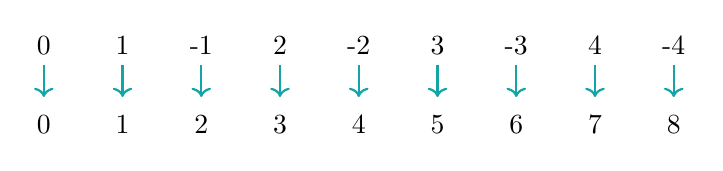
\begin{tikzpicture}

    % Draw the top row of numbers
    \node at (0, 0) {-2};
    \node at (1, 0) {3};
    \node at (-1, 0) {2};
    \node at (2, 0) {-3};
    \node at (-2, 0) {-1};
    \node at (3, 0) {4};
    \node at (-3, 0) {1};
    \node at (4, 0) {-4};
    \node at (-4, 0) {0};

    % Draw the second row of numbers (1, 2, 3, 4, ...)
    \node at (0, -1) {4};
    \node at (1, -1) {5};
    \node at (-1, -1) {3};
    \node at (2, -1) {6};
    \node at (-2, -1) {2};
    \node at (3, -1) {7};
    \node at (-3, -1) {1};
    \node at (4, -1) {8};
    \node at (-4, -1) {0};

    % Draw arrows from the top numbers to the bottom numbers
    \draw[->, teal, thick] (0, -0.25) -- (0, -0.65);
    \draw[->, teal, thick] (1, -0.25) -- (1, -0.65);
    \draw[->, teal, thick] (-1, -0.25) -- (-1, -0.65);
    \draw[->, teal, thick] (2, -0.25) -- (2, -0.65);
    \draw[->, teal, thick] (-2, -0.25) -- (-2, -0.65);
    \draw[->, teal, thick] (3, -0.25) -- (3, -0.65);
    \draw[->, teal, thick] (-3, -0.25) -- (-3, -0.65);
    \draw[->, teal, thick] (4, -0.25) -- (4, -0.65);
    \draw[->, teal, thick] (-4, -0.25) -- (-4, -0.65);

    \end{tikzpicture}
  \end{center}
\end{proof}

\begin{thm}
  $|\mathbb{Q}| = \aleph_0$
\end{thm}

\begin{proof}\leavevmode
  \begin{center}
    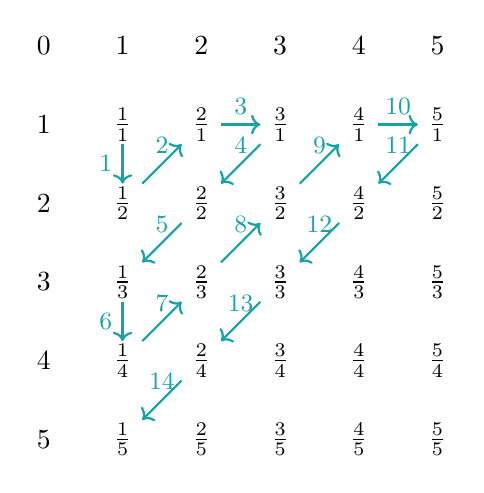
\begin{tikzpicture}

    \def\n{5};

    \foreach \a in {1, ..., \n} {
      \node at (-1, \n-\a) {\a};
    }

    \foreach \a in {1, ..., \n} {
      \node at (\a-1, \n) {\a};
    }

    \node at (-1, \n) {$0$};

    \foreach \a in {1, ..., \n} {
      \foreach \b in {1, ..., \n} {
        \node at (\a-1, -\b+\n) {$\frac{\a}{\b}$};
      }
    }

    \draw[->, teal, thick] (0, \n-1-0.25)       -- node[left]   {\small $1$}    (0, \n-2+0.25);
    \draw[->, teal, thick] (0+0.25, \n-2+0.25)  -- node[above]  {\small $2$}    (1-0.25, \n-1-0.25);
    \draw[->, teal, thick] (1+0.25, \n-1)       -- node[above]  {\small $3$}    (2-0.25, \n-1);
    \draw[->, teal, thick] (2-0.25, \n-1-0.25)  -- node[above]  {\small $4$}    (1+0.25, \n-2+0.25);
    \draw[->, teal, thick] (1-0.25, \n-2-0.25)  -- node[above]  {\small $5$}    (0+0.25, \n-3+0.25);
    \draw[->, teal, thick] (0, \n-3-0.25)       -- node[left]   {\small $6$}    (0, \n-4+0.25);
    \draw[->, teal, thick] (0+0.25, \n-4+0.25)  -- node[above]  {\small $7$}    (1-0.25, \n-3-0.25);
    \draw[->, teal, thick] (1+0.25, \n-3+0.25)  -- node[above]  {\small $8$}    (2-0.25, \n-2-0.25);
    \draw[->, teal, thick] (2+0.25, \n-2+0.25)  -- node[above]  {\small $9$}    (3-0.25, \n-1-0.25);
    \draw[->, teal, thick] (3+0.25, \n-1)       -- node[above]  {\small $10$}   (4-0.25, \n-1);
    \draw[->, teal, thick] (4-0.25, \n-1-0.25)  -- node[above]  {\small $11$}   (3+0.25, \n-2+0.25);
    \draw[->, teal, thick] (3-0.25, \n-2-0.25)  -- node[above]  {\small $12$}   (2+0.25, \n-3+0.25);
    \draw[->, teal, thick] (2-0.25, \n-3-0.25)  -- node[above]  {\small $13$}   (1+0.25, \n-4+0.25);
    \draw[->, teal, thick] (1-0.25, \n-4-0.25)  -- node[above]  {\small $14$}   (0+0.25, \n-5+0.25);

    \end{tikzpicture}
  \end{center}
\end{proof}

\begin{thm}
  $\mathbb{R}$ non è numerabile.
\end{thm}

\begin{proof}[Dimostrazione (Diagonalizzazione di Cantor)]
  Si dimostrerà che $[0, 1]$ non è numerabile. Si supponga di aver trovato un'enumerazione del suddetto insieme. È possibile 
  comunque trovare un nuovo numero nel seguente modo:

  \begin{center}
    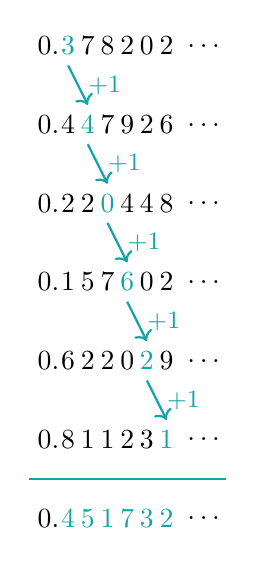
\begin{tikzpicture}

    \node at (-1, 4)  {$0.$};   \node at (-1+0.25, 4)  {$\color{teal} 3$};   \node at (-1+0.5, 4)  {$7$};   \node at (-1+0.75, 4)  {$8$};   \node at (-1+1, 4)  {$2$};   \node at (-1+1.25, 4)  {$0$};    \node at (-1+1.5, 4)  {$2$}; \node at (-1+2, 4)  {$\dots$};
    \node at (-1, 3)  {$0.$};   \node at (-1+0.25, 3)  {$4$};   \node at (-1+0.5, 3)  {$\color{teal} 4$};   \node at (-1+0.75, 3)  {$7$};   \node at (-1+1, 3)  {$9$};   \node at (-1+1.25, 3)  {$2$};    \node at (-1+1.5, 3)  {$6$}; \node at (-1+2, 3)  {$\dots$};
    \node at (-1, 2)  {$0.$};   \node at (-1+0.25, 2)  {$2$};   \node at (-1+0.5, 2)  {$2$};   \node at (-1+0.75, 2)  {$\color{teal} 0$};   \node at (-1+1, 2)  {$4$};   \node at (-1+1.25, 2)  {$4$};    \node at (-1+1.5, 2)  {$8$}; \node at (-1+2, 2)  {$\dots$};
    \node at (-1, 1)  {$0.$};   \node at (-1+0.25, 1)  {$1$};   \node at (-1+0.5, 1)  {$5$};   \node at (-1+0.75, 1)  {$7$};   \node at (-1+1, 1)  {$\color{teal} 6$};   \node at (-1+1.25, 1)  {$0$};    \node at (-1+1.5, 1)  {$2$}; \node at (-1+2, 1)  {$\dots$};
    \node at (-1, 0)  {$0.$};   \node at (-1+0.25, 0)  {$6$};   \node at (-1+0.5, 0)  {$2$};   \node at (-1+0.75, 0)  {$2$};   \node at (-1+1, 0)  {$0$};   \node at (-1+1.25, 0)  {$\color{teal} 2$};    \node at (-1+1.5, 0)  {$9$}; \node at (-1+2, 0)  {$\dots$};
    \node at (-1, -1) {$0.$};   \node at (-1+0.25,-1)  {$8$};   \node at (-1+0.5,-1)  {$1$};   \node at (-1+0.75,-1)  {$1$};   \node at (-1+1,-1)  {$2$};   \node at (-1+1.25,-1)  {$3$};    \node at (-1+1.5,-1)  {$\color{teal} 1$}; \node at (-1+2, -1)  {$\dots$};

    \draw[teal, thick] (-1-0.25, -1.5) -- (-1+2+0.25, -1.5);

    \draw[->, teal, thick] (-1+0.25, 4-0.25)       -- node[right]   {\small $+1$}    (-1+0.5, 3+0.25);
    \draw[->, teal, thick] (-1+0.5, 3-0.25)       -- node[right]   {\small $+1$}    (-1+0.75, 2+0.25);
    \draw[->, teal, thick] (-1+0.75, 2-0.25)       -- node[right]   {\small $+1$}    (-1+1, 1+0.25);
    \draw[->, teal, thick] (-1+1, 1-0.25)       -- node[right]   {\small $+1$}    (-1+1.25, 0+0.25);
    \draw[->, teal, thick] (-1+1.25, 0-0.25)       -- node[right]   {\small $+1$}    (-1+1.5, -1+0.25);

    \node at (-1, -2) {$0.$};   \node at (-1+0.25,-2)  {$\color{teal} 4$};   \node at (-1+0.5,-2)  {$\color{teal} 5$};   \node at (-1+0.75,-2)  {$\color{teal} 1$};   \node at (-1+1,-2)  {$\color{teal} 7$};   \node at (-1+1.25,-2)  {$\color{teal} 3$};    \node at (-1+1.5,-2)  {$\color{teal} 2$}; \node at (-1+2, -2)  {$\dots$};

    \end{tikzpicture}
  \end{center}
\end{proof}

\begin{thm}[Teorema di Cantor]
  Dato un qualsiasi insieme $A$ si ha che $|A| < |\wp{(A)}|$.
\end{thm}

\begin{obs}
  $|\wp{(\mathbb{N})}| = |\mathbb{R}|$. In particolare, $|\mathbb{R}|$ è 
  detta \textbf{cardinalità del continuo}.
\end{obs}

\begin{notation}
  $|\mathbb{R}| = \mathfrak{C}$
\end{notation}

\begin{proof}
  P.A. si supponga che esista $f: A \to \wp{(A)}$ biunivoca. Allora sia $B$ il sottoinsieme 
  di $A$ così definito:

  $$
    B := \{a \in A~\colon~a \not \in f(a)\}
  $$

  dato che $f$ è biunivoca, $\exists b \in A~\colon~f(b) = B$. 
  È facilmente verificabile che $b$ non può né appartenere né non appartenere a $B$, il che è un assurdo.
\end{proof}

\chapter{Trigonometria iperbolica}

\begin{define}[Coseno iperbolico]
  Si definisce \textbf{coseno iperbolico} la funzione $\cosh : \mathbb{R} \to \mathbb{R}$:

  $$
    \cos{x} := \dfrac{e^x + e^{-x}}{2}
  $$
\end{define}

\begin{define}[Seno iperbolico]
  Si definisce \textbf{seno iperbolico} la funzione $\sinh : \mathbb{R} \to \mathbb{R}$:

  $$
    \sinh{x} := \dfrac{e^x - e^{-x}}{2}
  $$
\end{define}

\begin{define}[Tangente iperbolica]
  Si definisce \textbf{tangente iperbolica} la funzione $\tanh : \mathbb{R} \to \mathbb{R}$:

  $$
    \tanh{x} := \dfrac{\sinh{x}}{\cosh{x}} = \dfrac{e^x - e^{-x}}{e^{x} + e^{-x}}
  $$
\end{define}

\begin{define}[Cotangente iperbolica]
  Si definisce \textbf{cotangente iperbolica} la funzione $\tanh : \mathbb{R}_0 \to \mathbb{R}$:

  $$
    \coth{x} := \dfrac{\cosh{x}}{\sinh{x}} = \dfrac{e^x + e^{-x}}{e^{x} - e^{-x}}
  $$
\end{define}

\begin{center}
\begin{tikzpicture}
\begin{groupplot}[
  group style={
    group size=2 by 1,
    horizontal sep=2.5cm,
    ylabels at=edge left,
    xlabels at=edge bottom,
    vertical sep=0pt
  },
  width=8.25cm,
  height=8.5cm,
  axis lines=middle,
  xlabel={$x$},
  samples=300,
  domain=-3:3,
  ticks=none,
  ymin=-3, ymax=6,
  legend style={font=\small, cells={anchor=west}},
  every axis title/.append style={yshift=-1ex}
]

\nextgroupplot[
  xmin=-2.5, xmax=2.5,
  ylabel={$y$},
  ylabel style={xshift=2.5pt}
]
\addplot[cmapteal-200, very thick] {sinh(x)};
\addlegendentry{$\sinh(x)$}
\addplot[cmapteal-400, very thick] {cosh(x)};
\addlegendentry{$\cosh(x)$}

\nextgroupplot[
  xmin=-3, xmax=3,
  ylabel={$y$}, 
  ylabel style={xshift=2.5pt}
]
\addplot[cmapteal-200, very thick] {tanh(x)};
\addlegendentry{$\tanh(x)$}
\addplot[cmapteal-400, very thick, domain=-3:-0.2] {cosh(x)/sinh(x)};
\addplot[cmapteal-400, very thick, domain=0.2:3] {cosh(x)/sinh(x)};
\addlegendentry{$\coth(x)$}

\end{groupplot}
\end{tikzpicture}
\end{center}


\begin{prop}\leavevmode
  $$
    \cosh^2{x} - \sinh^2{x} = 1~\forall x \in \mathbb{R}
  $$
\end{prop}

\begin{prop}
  Siano $\alpha, \beta \in \mathbb{R}$:

  \begin{itemize}
    \item $\sinh{(\alpha + \beta)} = \sinh{\alpha}\cosh{\beta} + \sinh{\beta}\cosh{\alpha}$
    \item $\cosh{(\alpha + \beta)} = \cosh{\alpha}\cosh{\beta} + \sinh{\alpha}\sinh{\beta}$
  \end{itemize}
\end{prop}

\begin{proof}

\end{proof}

\begin{cor}
  Siano $\alpha, \beta \in \mathbb{R}$:

  \begin{itemize}
    \item $\sinh{(\alpha - \beta)} = \sinh{\alpha}\cosh{\beta} - \sinh{\beta}\cosh{\alpha}$
    \item $\cosh{(\alpha - \beta)} = \cosh{\alpha}\cosh{\beta} - \sinh{\alpha}\sinh{\beta}$
  \end{itemize}
\end{cor}

\begin{cor}
  Sia $\alpha \in \mathbb{R}$:

  \begin{itemize}
    \item $\sinh{(2\alpha)} = 2\sinh{\alpha}\cosh{\alpha}$
    \item $\cosh{(2\alpha)} = \cosh^2{\alpha} + \sinh^2{\alpha}$
  \end{itemize}
\end{cor}

\begin{prop}
  Sia $\alpha \in \mathbb{R}$:

  \begin{itemize}
    \item $\sinh{\left(\dfrac{\alpha}{2}\right)} = \sgn{(\alpha)}\sqrt{\dfrac{\cosh{\alpha} - 1}{2}}$
    \item $\cosh{\left(\dfrac{\alpha}{2}\right)} = \sqrt{\dfrac{\cosh{\alpha} + 1}{2}}$
  \end{itemize}
\end{prop}

\begin{proof}

\end{proof}


\begin{prop}
  La funzione $\sinh : \mathbb{R} \to \mathbb{R}$ è invertibile e l'inversa è data da:
\end{prop}

\chapter{Numeri complessi}

\section{Introduzione}

\begin{define}
  Definiamo l'insieme dei numeri complessi $\mathbb{C}$ come:
  $$
    \mathbb{C} := \{x + iy~\colon~x, y \in \mathbb{R}\}
  $$
  con $i \in \mathbb{C}$ t.che $i^2 = -1$
\end{define}


\begin{define}
  Dato $z = a + ib \in \mathbb{C}$, definiamo \textbf{parte reale} e \textbf{parte immaginaria} di $z$ rispettivamente i numeri:

  $$
    \Re{(z)} = a
  $$
  $$
    \Im{(z)} = b
  $$
\end{define}


\begin{obs}
  $$
    z = w \iff  \begin{cases}
                  \Re{(z)} = \Re{(w)} \\
                  \Im{(z)} = \Im{(w)}
                \end{cases}
  $$
\end{obs}


\begin{define}
  Dati $z = a + ib$, $w = c + id$ con $a,b,c,d \in \mathbb{R}$,
  \begin{enumerate}
    \item $z + w = (a+b) + i(c+d)$
    \item $z \cdot w = (ac - bd) + i(bc + ad)$
    \item $|z| = \sqrt{a^2 + b^2}$
    \item $\conj{z} = a - ib$
  \end{enumerate}
\end{define}


\begin{property}
  Siano $z, w \in \mathbb{C}$,
  \begin{enumerate}
    \item $|z| \geqslant 0$ e $|z| = 0 \iff z = 0$
    \item $|z|^2 = |\conj{z}|^2 = z \cdot \conj{z}$
    \item $|z \cdot w| = |z||w|$
    \item $\Re{(z)} \leqslant |z|$, $\Im{(z)} \leqslant |z|$
  \end{enumerate}
\end{property}

\begin{proof}(3)
  \begin{align*}
    |z \cdot w|^2 &= (ac - bd)^2 + (bc + ad)^2 =  \\
                  &= (a^2c^2 + b^2d^2 - \cancel{2abcd}) + (a^2d^2 + b^2c^2 + \cancel{2abcd}) = \\
                  &= a^2(c^2 + d^2) + b^2(c^2 + d^2) = \\
                  &= (a^2 + b^2)(c^2 + d^2) = |z||w|
  \end{align*}
\end{proof}


\begin{thm}[Disuguaglianza triangolare]
  $$
    |z| + |w| \geqslant |z + w|~\forall z,w \in \mathbb{C}
  $$
\end{thm}

\begin{proof}
  Siano $z = a + ib$ e $w = c + id$, con $a,b,c,d \in \mathbb{R}$.

  \begin{align*}
    |z + w|^2 &= (a+c)^2 + (b+d)^2 = a^2 + c^2 + 2ac + b^2 + d^2 + 2bd = \\
              &= a^2 + b^2 + c^2 + d^2 + 2(ac + bd) = \\
              &= |z|^2 + |w|^2 + 2(\Re{(z\cdot \conj{w})}) \leqslant \\
              &\leqslant |z|^2 + |w|^2 + 2(|z\cdot \conj{w}|) = \\
              &= |z|^2 + |w|^2 + 2|z||w| = (|z| + |w|)^2
  \end{align*}
\end{proof}


\begin{prop}
  Sia $z \in \mathbb{C}$, $\exists z^* \in \mathbb{C}$ t.che $z \cdot z^* = 1$
\end{prop}

\begin{proof}
  Sia $z = a + ib$, 

  $$
    \dfrac{1}{z} = \dfrac{1}{a+ib} = \dfrac{1}{a+ib} \cdot \dfrac{a-ib}{a-ib} = \dfrac{a-ib}{a^2 + b^2} = \dfrac{a}{a^2+b^2} - i\dfrac{b}{a^2+b^2} = \dfrac{\conj{z}}{|z|^2} = z^*
  $$
\end{proof}

\begin{obs}
  Se $|z| = 1$, $z^* = \conj{z}$
\end{obs}


\begin{property}
  Siano $z, w \in \mathbb{C}$,

  \begin{enumerate}
    \item $\conj{\conj{z}} = z$
    \item $z = \conj{z} \iff z \in \mathbb{R}$
    \item $\conj{z + w} = \conj{z} + \conj{w}$
    \item $\conj{z\cdot w} = \conj{z}\cdot \conj{w}$
    \item $\conj{\dfrac{1}{z}} = \dfrac{z}{|z|^2}$
    \item $\Re{(z)} = \dfrac{z + \conj{z}}{2}$, $\Im{(z)} = \dfrac{z - \conj{z}}{2i}$
  \end{enumerate}
\end{property}


\section{Forma trigonometrica}

Un numero complesso può essere scritto in forma trigonometrica come:

$$
  z = \rho(\cos{\vartheta} + i\sin{\vartheta})
$$

con $\rho \in [0, +\infty)$, $\vartheta \in [-\pi, \pi)$

\begin{center}
\begin{tikzpicture}[scale=1.2, >=stealth]

  % Axes
  \draw[->, thick] (-2.5,0) -- (2.5,0) node[right] {$\Re(z)$};
  \draw[->, thick] (0,-2.5) -- (0,2.5) node[above] {$\Im(z)$};

  % Complex number z = 2 + i
  \coordinate (Z) at (2,1);
  \draw[thick, teal, ->] (0,0) -- (Z);
  \filldraw[teal] (Z) circle (2pt);
  \node[black, above right] at (Z) {$z$};
  \node[teal] at (1.0,0.8) {$\rho$};

  % Projections on axes
  \draw[dashed, gray] (Z) -- (2,0);
  \draw[dashed, gray] (Z) -- (0,1);

  % Argument angle
  \draw[->, thick, blue] (0.8,0) arc (0:26.565:0.8);
  \node[blue!80!black] at (1.2,0.3) {$\vartheta$};

  % Labels
  \node[below left] at (0,0) {$O$};

\end{tikzpicture}
\end{center}

\begin{lemma}\label{SinCosCProd}
  Siano $\vartheta, \varphi \in \mathbb{R}$, 

  $$
    (\cos{\vartheta} + i\sin{\vartheta})(\cos{\varphi} + i\sin{\varphi}) = \cos{(\vartheta + \varphi)} + +\sin{(\vartheta + \varphi)}
  $$
\end{lemma}

\begin{proof}

\end{proof}

\begin{obs}
  Siano $z, w \in \mathbb{C}$ con $|w| = 1$, allora geometricamente $z\cdot w$ equivale a ruotare $z$ di $\arg{w}$.
\end{obs}

\begin{thm}[Formula di De Moivre]
  Siano $z \in \mathbb{C}, n \in \mathbb{N}$, si ha che, detti $\rho = |z|$ e $\vartheta = \arg{z}$:

  $$
    z^n = \rho^n(\cos{n\vartheta} + i\sin{n\vartheta})
  $$
\end{thm}

\begin{proof}
  Per il lemma \ref{SinCosCProd}:
  $$
    z^n = \underset{n\text{ volte}}{\underbrace{z\cdot z\cdot \dots \cdot z}} = \rho^n(\cos{n\vartheta} + i\sin{n\vartheta})
  $$
\end{proof}

\begin{prop}
  Sia $z \in \mathbb{C}$ e $\arg{z} \in [-\pi, \pi)$:

  $$
    \arg{z} = 
    \begin{cases}
      \dfrac{\pi}{2}~\text{se}~\Re{(z)} = 0, \Im{(z)} > 0 \\[1em]
      -\dfrac{\pi}{2}~\text{se}~\Re{(z)} = 0, \Im{(z)} < 0 \\[1em]
      \arctan{\left[\dfrac{\Im{(z)}}{\Re{(z)}}\right]}~\text{se}~\Re{(z)} > 0 \\[1em]
      \arctan{\left[\dfrac{\Im{(z)}}{\Re{(z)}}\right]} + \pi ~\text{se}~\Re{(z)} < 0, \Im{(z)} \geqslant 0 \\[1em]
      \arctan{\left[\dfrac{\Im{(z)}}{\Re{(z)}}\right]} - \pi ~\text{se}~\Re{(z)} < 0, \Im{(z)} < 0 \\
    \end{cases} 
  $$
\end{prop}

\section{Radici $n$-esime}

\begin{define}[Esponenziale complesso]
  Sia $\lambda \in \mathbb{R}$, si definisce:

  $$
    e^{\lambda} := \cos{\lambda} + i\sin{\lambda}
  $$

  Sia $z \in \mathbb{C}$, si definisce:

  $$
    e^z := e^{\Re{(z)}}[\cos{\Im{(z)}} + i\sin{\Im{(z)}}]
  $$
\end{define}

\begin{define}
  Sia $z \in \mathbb{C}$, $w \in \mathbb{C}$ è una \textbf{radice $\boldsymbol{n}$-esima} di $z$, con $n \in \mathbb{N}$ se:
  
  $$
    w^n = z
  $$
\end{define}

\begin{obs}
  $e^{i\pi} = -1$, $e^{2\pi i} = 1$
\end{obs}

\begin{obs}[Forma esponenziale di un numero complesso]
  $$
    z = \rho(\cos{\vartheta} + i\sin{\vartheta}) = \rho e^{i\vartheta}
  $$
\end{obs}


\begin{thm}[Radici $n$-esime]
  Sia $n \in \mathbb{N}_0$ e $z = \rho e^{i\vartheta} \in \mathbb{C}_0$, $z$ ammette 
  $n$ radici distinte date da:

  $$
    w_k = \rho^{\frac{1}{n}}e^{i\vartheta_k},~~~\vartheta_k = \dfrac{\vartheta + 2k\pi}{n},~~~k\in \{0, 1, 2, \dots, n-1\}
  $$
\end{thm}

\begin{proof}
  Si provi prima che $w_k$ è una radice di $z$:

  $$
    w_k^{n} = (\rho^{\frac{1}{n}})^n e^{i\vartheta_k n} = \rho e^{i\vartheta}
  $$

  si mostri ora che $w_k$ sono le sole radici di $z$.

  $$
    t = \sqrt[n]{z} = z^{\frac{1}{n}} = \rho^{\frac{1}{n}} e^{i\frac{\vartheta}{n}}
  $$

  $$
    t = \rho^{\frac{1}{n}} e^{i\frac{\vartheta}{n}} \iff  \begin{cases}
                                                            |t| = \rho^{\frac{1}{n}} \\
                                                            \arg{t} = \dfrac{\vartheta}{n} + \dfrac{2k\pi}{n}
                                                          \end{cases}
  $$
  Sia:

  \begin{itemize}
    \item $k \in \{n, n+1, \dots\}$, allora:
          $$
            k = n\cdot q + r
          $$

          con $r \in \{0, 1, \dots, n-1\}$. Quindi:

          $$
            \arg{t} = \dfrac{\vartheta + 2\pi(nq + r)}{n}
          $$

          $$
            t = \rho^{\frac{1}{n}}e^{i\frac{\vartheta}{n}}e^{\frac{2\pi r}{n}}e^{2\pi q} = \rho^{\frac{1}{n}} e^{\frac{\vartheta + 2\pi r}{n}}
          $$

    \item $k \in \{-1, -2, \dots, -n+1\}$
  \end{itemize}
\end{proof}

\begin{center}
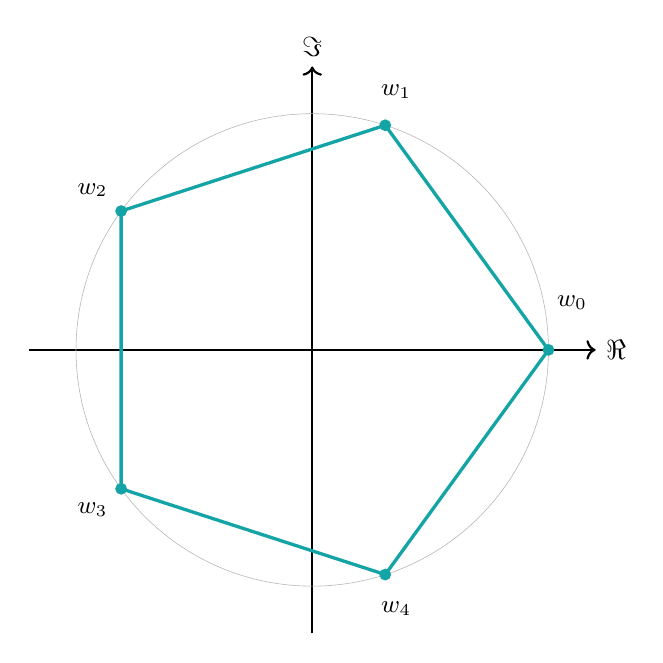
\begin{tikzpicture}[scale=3, thick]

  % Axes
  \draw[->, black] (-1.2,0) -- (1.2,0) node[right] {$\Re$};
  \draw[->, black] (0,-1.2) -- (0,1.2) node[above] {$\Im$};

  % Unit circle
  \draw[very thin, gray!60] (0,0) circle(1);

  % 5th roots of unity
  \foreach \k in {0,1,2,3,4} {
    \coordinate (P\k) at ({cos(360/5*\k)}, {sin(360/5*\k)});
    \filldraw[teal, z=10] (P\k) circle(0.02);
  }

  % Connect the points to form a pentagon
  \draw[teal, very thick] (P0) -- (P1) -- (P2) -- (P3) -- (P4) -- cycle;

  % Labels
  \foreach \k in {1,2,3,4} {
    \node[font=\small] at ($(0,0)!1.15!(P\k)$)
      {$w_{\k}$};
  }

  \node[font=\small] at (1.1, 0.2)
      {$w_{0}$};

\end{tikzpicture}
\end{center}


\begin{define}[Molteplicità]
  Sia $p_n(z)$ un polinomio, con $n \in \mathbb{N}$, $z \in \mathbb{C}$ e sia $\alpha \in \mathbb{C}~\colon~p_n(\alpha) = 0$. 
  Si dice \textbf{molteplicità} di $\alpha$ l'esponente di $(z-\alpha)$ nella fattorizzazione di $p_n(z)$.
\end{define}


\begin{prop}
  L'equazione a coefficienti reali:

  $$
    a_0 + a_1z + a_2z^2 + \dots + a_nz^n = 0,~~~a_i \in \mathbb{R}
  $$

  soddisfa le seguenti proprietà:

  \begin{itemize}
    \item Se $z$ è soluzione se e solo se $\conj{z}$ è soluzione
    \item Se $z$ è soluzione, $z$ e $\conj{z}$ hanno la stessa molteplicità
  \end{itemize}
\end{prop}

\begin{proof}\leavevmode
  \begin{itemize}
    \item Sia $\alpha \in \mathbb{C}$ soluzione, allora:

          $$
            a_0 + a_1\alpha + a_2\alpha^2 + \dots + a_n\alpha^n = 0,~~~a_i \in \mathbb{R}
          $$
          $$
            \conj{a_0 + a_1\alpha + a_2\alpha^2 + \dots + a_n\alpha^n} = \conj{0}
          $$
          $$
            a_0 + a_1\conj{\alpha} + a_2\conj{\alpha}^2 + \dots + a_n\conj{\alpha}^n = 0
          $$
    \item Supponiamo che $\alpha$ sia soluzione, ma $\equalto{m(\alpha)}{s} > \equalto{m(\conj{\alpha})}{t}$. Allora il polinomio associato può 
          essere scritto come:

          $$
            p_n(z) = (z - \alpha)^s(z - \conj{\alpha})^tq_n(z)
          $$

          Sia: 
          
          $$
            \widetilde{p}(z) = \dfrac{p_n(z)}{(z-\alpha)^t(z-\conj{\alpha})^t} = (z-\alpha)^{s-t}q_n(z)
          $$

          allora $\widetilde{p}(z)$ è un polinomio a coefficienti reali ed ha $\alpha$ come radice, ma non $\conj{\alpha}$. Ciò contraddice 
          il punto precedente.
  \end{itemize}
\end{proof}


\begin{thm}[Teorema fondamentale dell'algebra]
  Siano $a_0, a_1, \dots, a_n \in \mathbb{C}$ con $a_n \neq 0$, l'equazione:
  
  $$
    a_0 + a_1z + a_2z^2 + \dots + a_nz^n = 0
  $$

  ha esattamente $n$ soluzioni in $\mathbb{C}$, contate con le loro molteplicità. 
  Si dice che $\mathbb{C}$ è un campo \textbf{algebricamente chiuso}.
\end{thm}


\section{Struttura algebrica di $\mathbb{C}$}



\chapter{Successioni}


\section{Introduzione}

\begin{defineimp}
  Si definisce una \textbf{successione} $\{a_n\}$ una funzione $a\colon \mathbb{N} \to \mathbb{R}$.
\end{defineimp}

\begin{define}
  Una successione $a_n$ è \textbf{positiva} se $a_n \geqslant 0~\forall n$
\end{define}

\begin{define}
  Una successione $a_n$ è \textbf{limitata} se:

  $$
    \exists M > 0~\colon~|a_n| \leqslant M~\forall n
  $$
\end{define}

\begin{center}
\begin{tikzpicture}
  \begin{axis}[
      width=12cm,
      height=7cm,
      xmin=0, xmax=20,
      ymin=-0.5, ymax=2.5,
      axis lines=middle,
      xlabel={$n$},
      ylabel={$a_n$},
      % xtick={0,5,10,15,20},
      % ytick={0,1,2},
      ticks=none,
      domain=0:20,
      samples=40,
      clip=false,
    ]

    % Upper and lower bounds
    \addplot [name path=upper, very thick, dashed, color=cmapteal-300] {2};
    \addplot [name path=lower, very thick, dashed, color=cmapteal-300] {0};

    % Bounded sequence (sample data)
    \addplot [
      only marks,
      mark=*,
      cmapteal-400,
    ] table {
      1 1.84
      2 1.91
      3 1.14
      4 0.24
      5 0.04
      6 0.72
      7 1.65
      8 1.98
      9 1.41
      10 0.54
      11 0.09
      12 0.47
      13 1.40
      14 1.94
      15 1.56
      16 0.75
      17 0.16
      18 0.34
      19 1.20
      20 1.89
    };

    % Labels
    \node[cmapteal-300, anchor=west] at (axis cs:20,2) {$M$};
    \node[cmapteal-300, anchor=west] at (axis cs:20,0) {$M$};
    \node[cmapteal-400, anchor=west] at (axis cs:15,1.5) {$(a_n)$};

  \end{axis}
\end{tikzpicture}
\end{center}

\begin{define}
  Data una proposizione $P(n)$, con $n \in \mathbb{N}$, è vera \textbf{definitivamente} se è vera $\forall n \geqslant n_0$, con $n_0 \in \mathbb{N}$.
\end{define}


\begin{defineimp}
  Data una successione $a_n$, si dice che $a_n$ \textbf{converge}, oppure tende a, oppure ha limite $l \in \mathbb{R}$ se $\exists l \in \mathbb{R}$ t.che:
  $$
    \forall \varepsilon > 0~\exists n_0 \in \mathbb{N}~\colon~|a_n - l| < \varepsilon~\forall n \geqslant n_0
  $$
\end{defineimp}

\begin{center}
\begin{tikzpicture}
  \begin{axis}[
      width=13cm,
      height=7cm,
      xmin=0, xmax=20,
      ymin=-0.5, ymax=2.5,
      axis lines=middle,
      xlabel={$n$},
      ylabel={$a_n$},
      ticks=none,
      domain=0:20,
      samples=40,
      clip=false,
    ]

    % Define limit and epsilon band
    \def\L{1.2}
    \def\eps{0.2}
    \def\n0{4}

    % Epsilon tube (the "tube" around the limit)
    \addplot [
      name path=upper,
      draw=none,
      domain=\n0:20,
    ] { \L + \eps };

    \addplot [
      name path=lower,
      draw=none,
      domain=\n0:20,
    ] { \L - \eps };

    \addplot [
      fill=cmapteal-200,
      opacity=0.4,
    ] fill between[of=upper and lower];

    % Upper and lower bounds of the tube
    \addplot [very thick, dashed, color=cmapteal-300] { \L + \eps };
    \addplot [very thick, dashed, color=cmapteal-300] { \L - \eps };

    \draw [very thick, dashed, color=cmapteal-300] (\n0, 0) -- (\n0, \L + \eps);
    \node[below, cmapteal-300] at (\n0, 0) {$n_0$};

    % Converging sequence points
    \addplot [
      only marks,
      mark=*,
      color=cmapteal-400,
    ] table {
      1 2.0
      2 1.8
      3 1.6
      4 1.45
      5 1.35
      6 1.28
      7 1.23
      8 1.22
      9 1.21
      10 1.20
      11 1.19
      12 1.20
      13 1.21
      14 1.20
      15 1.20
      16 1.19
      17 1.20
      18 1.21
      19 1.20
      20 1.20
    };

    % Limit line
    \addplot [very thick, color=blue!70!black] { \L };
    \node[anchor=west, blue!70!black] at (axis cs:20,\L) {$L$};

    % Labels
    \node[cmapteal-400, anchor=west] at (axis cs:10,1.6) {$(a_n)$};
    \node[teal!60!black, anchor=west] at (axis cs:20,\L+\eps) {$L + \varepsilon$};
    \node[teal!60!black, anchor=west] at (axis cs:20,\L-\eps) {$L - \varepsilon$};

  \end{axis}
\end{tikzpicture}
\end{center}

\begin{thm}
  $a_n \to l \in \mathbb{R}$ $\iff$ $|a_n - l| \to 0$.
\end{thm}

\begin{proof}
  Dato che $|a_n - l| \to 0$, si ha che:

  $$
    \forall \varepsilon > 0~\exists n_0~\colon~||a_n - l| - 0| < \varepsilon~\forall n \geqslant n_0
  $$

  ne segue che

  $$
    \forall \varepsilon > 0~\exists n_0~\colon~|a_n - l| < \varepsilon~\forall n \geqslant n_0
  $$

  quindi $a_n \to l$
\end{proof}

\begin{thm}
  Sia $\{a_n\}$ definitivamente positiva. Se $a_n \to a \in \mathbb{R}$, $\sqrt{a_n} \to \sqrt{a}$.
\end{thm}

\begin{proof}
  Si noti che dati $x, y \in \mathbb{R}^+$, si ha:

  $$
    |\sqrt{x} - \sqrt{y}| \leqslant \sqrt{|x - y|}
  $$

  quindi:

  $$
    |\sqrt{a_n} - \sqrt{a}| \leqslant \sqrt{|a_n - a|}
  $$

  dato che $a_n \to a$, si ha che, fissato $\varepsilon > 0$:

  $$
    |a_n - a| < \varepsilon~\definit \implies \sqrt{|a_n - a|} < \sqrt{\varepsilon}~\definit
  $$

  preso $\varepsilon' = \sqrt{\varepsilon}$, ciò dimostra la tesi.

  $$
    |\sqrt{a_n} - \sqrt{a}| < \varepsilon'~\definit
  $$
  
\end{proof}

\begin{thm}
  Sia $\{a_n\}$. Se $a_n \to a \in \mathbb{R}$, $|a_n| \to |a|$.
\end{thm}

\begin{proof}

  Si noti che dati $a, b \in \mathbb{R}$, si ha:

  $$
    ||a| - |b|| \leqslant |a-b|
  $$

  quindi:

  $$
    ||a_n| - |a|| \leqslant |a_n - a|
  $$

  dato che $a_n \to a$, si ha che, fissato $\varepsilon > 0$:
  
  $$
    |a_n - a| < \varepsilon~\definit \implies ||a_n| - |a|| < \varepsilon~\definit
  $$
  
\end{proof}


\begin{define}
  Data una successione $a_n$, diciamo che $a_n$ \textbf{diverge}, oppure tende a, oppure ha limite $+\infty$ se:

  $$
    \forall M > 0~\exists n_0 \in \mathbb{N}~\colon~a_n > M~\forall n \geqslant n_0
  $$
\end{define}


\section{Unicità del limite}

\begin{thmimp}
  Se $a_n \to l \in \mathbb{R}$, $l$ è unico.
\end{thmimp}

\begin{proof}
  P.A. supponiamo che esistano due numeri reali $l_1$ e $l_2$, tali che $l_1 \neq l_2$ e tali che:

  \begin{center}
    $\forall \varepsilon > 0~\exists n_1 \in \mathbb{N}~\colon~|a_n - l_1| < \varepsilon~\forall n \geqslant n_1$\\
    $\forall \varepsilon > 0~\exists n_2 \in \mathbb{N}~\colon~|a_n - l_2| < \varepsilon~\forall n \geqslant n_2$
  \end{center}

  Sia $\varepsilon = \dfrac{|l_1 - l_2|}{3}$, si ha che:

  $$
    |l_1 - l_2| = |l_1 - a_n + a_n - l_2| \leqslant |l_1 - a_n| + |l_2 - a_n| < 2\varepsilon~\definit
  $$
  $$
    \implies |l_1 - l_2| < 2\varepsilon = 2\dfrac{|l_1 - l_2|}{3} \implies 1 < \dfrac{2}{3}
  $$

  il che è un assurdo.

  
  \begin{center}
  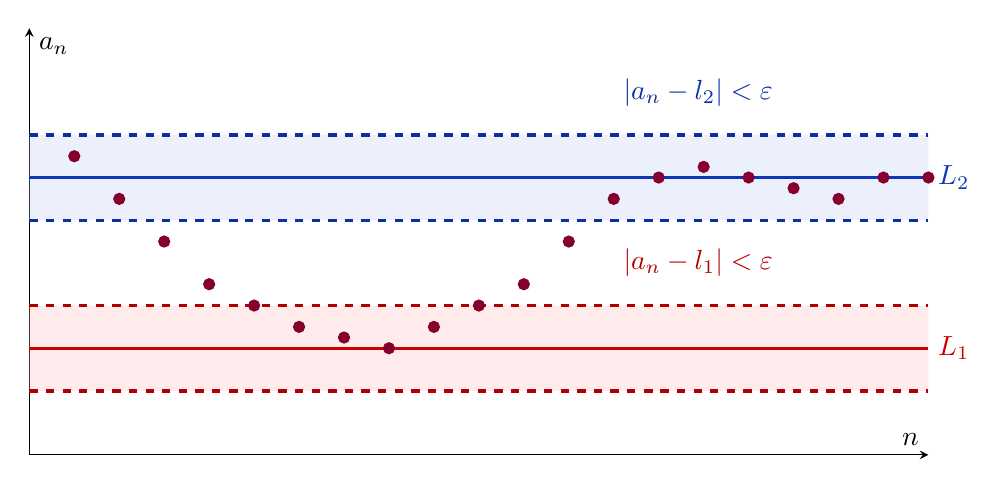
\begin{tikzpicture}
    \begin{axis}[
        width=13cm,
        height=7cm,
        xmin=0, xmax=20,
        ymin=0.5, ymax=2.5,
        axis lines=middle,
        xlabel={$n$},
        ylabel={$a_n$},
        ticks=none,
        domain=0:20,
        samples=40,
        clip=false,
      ]

      % Define two hypothetical limits
      \def\Lone{1.0}
      \def\Ltwo{1.8}
      \def\eps{0.2}

      % Epsilon neighborhoods for L1 and L2
      \addplot [name path=upperA, draw=none] { \Lone + \eps };
      \addplot [name path=lowerA, draw=none] { \Lone - \eps };
      \addplot [fill=red!20, opacity=0.4] fill between[of=upperA and lowerA];

      \addplot [name path=upperB, draw=none] { \Ltwo + \eps };
      \addplot [name path=lowerB, draw=none] { \Ltwo - \eps };
      \addplot [fill=blue!20, opacity=0.4] fill between[of=upperB and lowerB];

      % Dashed bounds for epsilon bands
      \addplot [very thick, dashed, color=red!70!black] { \Lone + \eps };
      \addplot [very thick, dashed, color=red!70!black] { \Lone - \eps };
      \addplot [very thick, dashed, color=blue!70!black] { \Ltwo + \eps };
      \addplot [very thick, dashed, color=blue!70!black] { \Ltwo - \eps };

      % Sequence (points "trying" to converge)
      \addplot [
        only marks,
        mark=*,
        color=purple!70!black,
      ] table {
        1 1.9
        2 1.7
        3 1.5
        4 1.3
        5 1.2
        6 1.1
        7 1.05
        8 1.0
        9 1.1
        10 1.2
        11 1.3
        12 1.5
        13 1.7
        14 1.8
        15 1.85
        16 1.8
        17 1.75
        18 1.7
        19 1.8
        20 1.8
      };

      % Limit lines and labels
      \addplot [very thick, color=red!80!black] { \Lone };
      \addplot [very thick, color=blue!80!black] { \Ltwo };

      \node[red!80!black, anchor=west] at (axis cs:20,\Lone) {$L_1$};
      \node[blue!80!black, anchor=west] at (axis cs:20,\Ltwo) {$L_2$};

      % Annotate disjoint neighborhoods
      \node[anchor=west, red!70!black] at (axis cs:13,\Lone+0.4)
        {$|a_n - l_1| < \varepsilon$};
      \node[anchor=west, blue!70!black] at (axis cs:13,\Ltwo+0.4)
        {$|a_n - l_2| < \varepsilon$};

      % \draw[<->, thick, gray!70!black] (axis cs:19,\Lone+\eps) -- (axis cs:19,\Ltwo-\eps)
      %   node[midway, right, text=gray!70!black] {disjoint bands};

    \end{axis}
  \end{tikzpicture}
  \end{center}
\end{proof}

\section{Permanenza del segno}

\begin{thmimp}
  Sia $a_n \to l$, si ha che:
  \begin{itemize}
    \item Se $l > 0$, $a_n > 0~\definit$
    \item Se $a_n \geqslant 0~\definit$, allora $l \geqslant 0$;
  \end{itemize}
\end{thmimp}

\begin{proof}\leavevmode
  \begin{itemize}
    \item Sia $\varepsilon = \dfrac{l}{2}$. Si ha che:

    $$
      0 < |a_n - l| < \dfrac{l}{2} \implies 0 < \dfrac{l}{2} < a_n < \dfrac{3l}{2}
    $$
  
    \item In modo analogo, se $l < 0$, $a_n < 0$, quindi se $a_n \geqslant 0$, $l \geqslant 0$.
  \end{itemize}
\end{proof}


\section{Teorema del confronto}

\begin{thmimp}[Primo teorema del confronto]
  Siano $\{a_n\}$, $\{b_n\}$ e $\{c_n\}$ tre successioni tali che:

  $$
    a_n \leqslant c_n \leqslant b_n~\definit
  $$

  se $a_n \to l$, $b_n \to l$ con $l \in \mathbb{R}$, allora $c_n \to l$.
\end{thmimp}

\begin{proof}
  Dato che $a_n$ e $b_n$ convergono allo stesso $l$:

  $$
    \forall \varepsilon' > 0~\exists n_0'~\colon~ -\varepsilon' + l < a_n < \varepsilon' + l ~\forall n \geqslant n_0'
  $$
  $$
    \forall \varepsilon'' > 0~\exists n_0''~\colon~ -\varepsilon'' + l < b_n < \varepsilon'' + l~\forall n \geqslant n_0''
  $$

  sia ora $n_0 = \max{\{n_0', n_0''\}}$, dato che $a_n \leqslant b_n$:

  $$
    \forall \varepsilon'~\forall \varepsilon''~\exists n_0~\colon~-\varepsilon' + l < a_n \leqslant b_n < \varepsilon'' + l~\forall n \geqslant n_0
  $$
  $$
    \forall \varepsilon'~\forall \varepsilon''~\exists n_0~\colon~-\varepsilon' + l < a_n \leqslant c_n \leqslant b_n < \varepsilon'' + l~\forall n \geqslant n_0
  $$

  per giungere a $c_n \to l$, basta prendere $\varepsilon = \min{\{\varepsilon', \varepsilon''\}}$.
\end{proof}

\begin{thm}[Secondo teorema del confronto]
  Siano $\{a_n\}$ e $\{b_n\}$ due successioni tali che:

  $$
    a_n \leqslant b_n~\definit
  $$

  se $a_n \to \infty$, allora $b_n \to \infty$.
\end{thm}

\begin{proof}
  Dato che $a_n \to \infty$, si ha che:

  $$
    \forall M > 0~\exists n_0~\colon~a_n > M~\forall n \geqslant n_0
  $$

  avendo $b_n \geqslant a_n$:

  $$
    \forall M > 0~\exists n_0~\colon~M < a_n \leqslant b_n~\forall n \geqslant n_0
  $$
\end{proof}


\begin{cor}
  Se $\{a_n\}$ è una successione limitata e $\{\varepsilon_n\}$ è una successione 
  infinitesima, $a_n \cdot \varepsilon_n \to 0$
\end{cor}

\begin{proof}
  Dato che $a_n$ è limitata:

  $$
    \exists M > 0~\colon~-M \leqslant a_n \leqslant M~\forall n
  $$

  si supponga $\varepsilon_n > 0~\definit$ (ciò tuttavia non fa perdere di generalità). Allora: 

  $$
    \exists M > 0~\colon~-M\cdot \varepsilon_n \leqslant a_n\cdot \varepsilon_n \leqslant M \cdot \varepsilon_n~\forall n
  $$

  Quindi $a_n \cdot \varepsilon_n \to 0$ per il teorema del confronto.
\end{proof}


\section{Monotonia}

\begin{define}
  Data una successione $\{a_n\}$, diciamo che essa è \textbf{monotona}:

  \begin{itemize}
    \item \textbf{crescente} se $a_{n+1} \geqslant a_{n}~\forall n$;
    \item \textbf{strettamente crescente} se $a_{n+1} > a_{n}~\forall n$;
    \item \textbf{decrescente} se $a_{n+1} \leqslant a_{n}~\forall n$;
    \item \textbf{strettamente decrescente} se $a_{n+1} < a_{n}~\forall n$.
  \end{itemize}
\end{define}


\begin{thm}
  Se una successione $\{a_n\}$ è definitivamente monotona, allora è regolare. In particolare:

  \begin{itemize}
    \item Se $\{a_n\}$ è illimitata, $\{a_n\}$ diverge.
    \item Se $\{a_n\}$ è limitata, $\{a_n\}$ converge;
  \end{itemize}
\end{thm}

\begin{proof}\leavevmode
  \begin{itemize}
    \item Consideriamo il caso in cui $\{a_n\}$ sia monotona crescente. Dato che non è limitata, si ha che:
          $$
            \forall M > 0~\exists a_{n_0}~\colon~|a_{n_0}| > M
          $$
          dato che $\{a_n\}$ è crescente, $a_n \geqslant a_{n_0}~\forall n \geqslant n_0$. Quindi:

          $$
            \forall M > 0~\exists n_0~\colon~a_n > M~\forall n \geqslant n_0
          $$
    \item Consideriamo nuovamente il caso in cui $\{a_n\}$ sia crescente. Sia:
          $$
            A = \{a_0, a_1, \dots\}
          $$
          per la completezza di $\mathbb{R}$, $A$ ammette estremo superiore. Sia $\gamma = \sup_{A}$. Per la definizione di estremo superiore:

          $$
            \forall \varepsilon > 0~\exists a_{n_0} \in A~\colon~\gamma - \varepsilon < a_{n_0}
          $$
          Dato che $\{a_n\}$ è crescente:
          $$
            \forall \varepsilon > 0~\exists n_0~\colon~\gamma - a_n < \varepsilon~\forall n \geqslant n_0
          $$
          $$
            \forall \varepsilon > 0~\exists n_0~\colon~\gamma - \varepsilon < a_n \leqslant \gamma~\forall n \geqslant n_0
          $$
  \end{itemize}
\end{proof}


\begin{notation}
  $a_n \uparrow \gamma$, $b_n \downarrow \gamma$ ($a_n$ tende a $\gamma$ dal basso, $b_n$ tende a $\gamma$ dall'alto)
\end{notation}


\section{Numero di Eulero}

\begin{define}
  $$
    e_n = \left(1 + \dfrac{1}{n}\right)^n
  $$
\end{define}

\begin{thm}
  $e_n$ converge.
\end{thm}

\begin{proof}
  Dimostriamo che $e_n$ è monotona crescente:

  \begin{align*}
    a_{n+1} \geqslant a_n &\iff \left(1 + \dfrac{1}{n+1}\right)^{n+1} \geqslant \left(1 + \dfrac{1}{n}\right)^n \\
                          &\iff \left[\dfrac{1 + \dfrac{1}{n+1}}{1 + \dfrac{1}{n}}\right]^{n+1} \geqslant \dfrac{1}{1 + \dfrac{1}{n}} \\
                          &\iff \left[\dfrac{\dfrac{n+2}{n+1}}{\dfrac{n+1}{n}}\right]^{n+1} \geqslant \dfrac{n}{n+1} \\
                          &\iff \left[\dfrac{n(n+2)}{(n+1)^2}\right]^{n+1} \geqslant 1 - \dfrac{1}{n+1} \\
                          &\iff \left[\dfrac{n^2 + 2n + 1 - 1}{n^2 + 2n + 1}\right]^{n+1} \geqslant 1 - \dfrac{1}{n+1} \\
                          &\iff \left[1 - \dfrac{1}{(n+1)^2}\right]^{n+1} \geqslant 1 - \dfrac{1}{n+1} \\
  \end{align*}

  che è la disuguaglianza di Bernoulli con $x = -\dfrac{1}{(n+1)^2}$.

  In modo analogo si dimostra che $\displaystyle \left(1 + \dfrac{1}{n}\right)^{n+1}$ è decrescente.

  Dato che $e_n < \displaystyle \left(1 + \dfrac{1}{n}\right)^{n+1}~\forall n$, $e_n$ è superiormente limitata. Dato che $e_n$ è monotona, ne segue che $e_n$ 
  converge.
\end{proof}

\begin{define}[Numero di Eulero]
  $e := \lim{e_n}$
\end{define}


\section{Sottosuccessioni}

\begin{defineimp}
  Data una successione $a_n$ e una successione $n_k: \mathbb{N} \to \mathbb{N}$, si dice \textbf{sottosuccessione} di $a_n$ la funzione composta 
  $a_{n_k} = a_n \circ n_k$
\end{defineimp}

\begin{obs}
  Le possibili Sottosuccessioni di una data successione $a_n$ sono infinite di cardinalità $\mathfrak{C}$
\end{obs}

\begin{thm}
  Se una successione $a_n \to l \in \overline{\mathbb{R}}$, allora ogni sottosuccessione $a_{n_k} \to l$.
\end{thm}

\begin{obs}
  Se una successione $a_n$ ammette due Sottosuccessioni che hanno limite diverso, $a_n$ è oscillante.
\end{obs}

\begin{lemma}[Lemma dei picchi]
  Ogni successione ammette una sottosuccessione monotona.
\end{lemma}

\begin{proof}
  Sia $\{a_n\}$ una generica successione. Definiamo \textit{picco} una coppia $(n_0, a_{n_0})$ se $a_{n_0} \geqslant a_{n}~\forall n \geqslant n_0$. 

  \begin{center}
  \begin{tikzpicture}
    \begin{axis}[
      width=10cm,
      height=7cm,
      axis lines=middle,
      xlabel={$n$},
      ylabel={$a_n$},
      samples=10,
      domain=0:9,
      xtick=\empty, % Hide x ticks
      ytick=\empty, % Hide y ticks
      grid=both,
      every axis label/.append style={font=\small},
    ]
    % Plotting the sequence
    \addplot[cmapteal-500, mark=*, thick] coordinates {
      (0,2) (1,3) (2,6) (3,4) (4,5) (5,3) (6,4) (7,4.5) (8,3) (9,2.5)
    };
    
    % Highlighting peaks
    \addplot[only marks, mark=*, mark options={fill=tyrian, scale=1.5}] coordinates {
      (2,6) (4,5) (7,4.5)
    };

    \end{axis}
  \end{tikzpicture}
  \end{center}

  La successione $a_n$ può quindi avere:

  \begin{itemize}
    \item Un numero infinito di picchi. In tal caso, si costruisca una sottosuccessione di $a_n$ che abbia come elementi i 
          picchi. In tal modo, la sottosuccessione sarà decrescente (per la definizione di picco) e quindi monotona.
    \item Un numero finito di picchi. In tal caso si prenda l'ultimo picco (quello con $n_0$ maggiore). Si ha che 
          $\exists n_1 > n_0+1~\colon~a_{n_1} > a_{n_0+1}$ (altrimenti $(n_0 + 1, a_{n_0 + 1})$ sarebbe un picco). Si può così 
          iterare la procedura e costruire una sottosuccessione crescente.
  \end{itemize}
\end{proof}

\begin{thmimp}[Teorema di Bolzano-Weierstrass]
  Ogni successione limitata ammette una sottosuccessione convergente.
\end{thmimp}

\begin{proof}
  Per il \textit{lemma dei picchi} ogni successione $a_n$ ammette una sottosuccessione $a_{n_k}$ monotona. 
  Per un teorema precedentemente dimostrato, se $a_{n_k}$ è monotona è limitata, allora converge.
\end{proof}


\section{Limite superiore e limite inferiore}

\begin{define}
  Sia $a_n$ una successione, si definisce \textbf{limite superiore} di $a_n$:

  $$
    \lim_{m \to \infty}\left(\sup_{m \geqslant n}{a_n}\right)
  $$
\end{define}

\begin{define}
  Sia $a_n$ una successione, si definisce \textbf{limite inferiore} di $a_n$:

  $$
    \lim_{m \to \infty}\left(\inf_{m \geqslant n}{a_n}\right)
  $$
\end{define}

\begin{notation}
  $\limsup a_n$, $\liminf a_n$, $\overline{\lim{}} a_n$, $\underline{\lim{}} a_n$
\end{notation}

\begin{define}
  Sia $a_n$ una successione, $l \in \overline{\mathbb{R}}$ è \textbf{limite sottosuccesionale} di $a_n$ se 
  $\exists a_{n_k} \to l$.
\end{define}

\begin{property}
$$
  \underline{\lim{}} a_n \leqslant \overline{\lim{}} a_n
$$
In particolare, se $\underline{\lim{}} a_n = \overline{\lim{}} a_n$, $a_n \to \underline{\lim{}} a_n = \overline{\lim{}} a_n$.
\end{property}

\begin{thm}
  Il limite superiore è il più grande limite sottosuccesionale possibile di una successione.
\end{thm}


\section{Proprietà dei limiti}

\begin{thm}[Operazioni con i limiti]
  Siano $a_n \to a \in \mathbb{R}$, $b_n \to b \in \mathbb{R}$:
  \begin{enumerate}
    \item $a_n + b_n \to a + b$
    \item $a_n \cdot b_n \to a\cdot b$
    \item Se $b \neq 0$, $\dfrac{a_n}{b_n} \to \dfrac{a}{b}$
  \end{enumerate}
\end{thm}

\begin{proof}\leavevmode
  \begin{enumerate}
    \item $$
            |a_n + b_n - (a+b)| = |a_n - a + b_n - b| \leqslant |a_n - a| + |b_n - b| < 2\varepsilon~\forall \varepsilon~\definit
          $$
    \item \begin{align*}
            |a_n\cdot b_n - a\cdot b| &= |a_nb_n - a_nb + a_nb - ab| = |a_n(b_n - b) + b(a_n - a)| \leqslant \\
                                      &\leqslant |a_n||b_n - b| + |b||a_n - a|
          \end{align*}
          dato che $a_n \to a$, $|b||a_n - a| \to 0$. Dato che $a_n$ converge, $|a_n|$ converge ed è limitata. Quindi $|a_n||b_n - b| \to 0$. 
          Quindi $|a_n - ab| \to 0$ per confronto $\implies$ $a_nb_n \to ab$.
    \item Per il terzo punto, basta provare che $\dfrac{1}{b_n} \to \dfrac{1}{b}$:
          \begin{align*}
            \left|\dfrac{1}{b_n} - \dfrac{1}{b}\right| &= \left|\dfrac{b - b_n}{b_nb}\right| = |b_n - b|\dfrac{1}{|b_n||b|} \leqslant \dfrac{2}{|b^2|}|b_n - b| \to 0
          \end{align*}
          dove nell'utlimo passaggio si è utilizzato il fatto che se $|b_n| \to |b|$ allora $|b_n| \geqslant \dfrac{|b|}{2}~\definit$
  \end{enumerate}
\end{proof}


\begin{prop}
  $\sin{n}$ non converge.
\end{prop}

\begin{proof}
  P.A. si supponga che $\sin{n} \to l \in [-1, 1]$ (se $\sin{n}$ converge ad $l$, per 
  il teorema della permanenza del segno si deve avere $-1 \leqslant l \leqslant 1$). \\

  Si considerino:

  $$
    \sin{(n+1)} = \sin{n}\cdot\cos{1} + \sin{1}\cdot\cos{n} \to l
    \sin{(n-1)} = \sin{n}\cdot\cos{1} - \sin{1}\cdot\cos{n} \to l
  $$
  
  entrambe convergono ad $l$ poiché sottosuccessioni di $\sin{n}$. Quindi:

  $$
    \sin{(n+1)} + \sin{(n-1)} = 2\sin{n}\cdot\cos{1} \implies l + l = 2l\cdot\cos{1}
  $$

  dato che $\cos{1} \neq 1$, $l = 0$. Si consideri ora:

  $$
    \sin{(n+1)} - \sin{(n-1)} = 2\sin{1}\cdot\cos{n} \to l - l = 0
  $$

  dato che $\sin{1} \neq 0$, $\cos{n} \to 0$. Ma si ha che:

  $$
    \sin^2{n} + \cos^2{n} \to 0 + 0 \neq 1
  $$

  ciò è un assurdo.
\end{proof}


\section{Aritmetica estesa}

\begin{itemize}
  \item $+\infty + \infty = +\infty$
  \item $+\infty \cdot c = +\infty~c \in \mathbb{R}^+$
  \item $+\infty \cdot (-c) = -\infty~c \in \mathbb{R}^+$
  \item $\dfrac{c}{+\infty} = 0^+~c \in \mathbb{R}^+$
  \item $\dfrac{c}{0^+} = +\infty~c \in \mathbb{R}^+$
  \item $[\dots]$
\end{itemize}

\subsection{Forme indeterminate}

\begin{enumerate}
  \item $+\infty \cdot 0$
  \item $+\infty - \infty$
  \item $\dfrac{+\infty}{+\infty}$
  \item $\dfrac{0}{0}$
  \item $1^{\infty}$
  \item $\infty^0$
  \item $0^0$
\end{enumerate}

Si noti che le ultime tre possono essere ricondotte alle 2., 3. e 4., che a loro volta possono essere ricondotte alla prima.


\section{Limiti notevoli}

Sia $\varepsilon_n \to 0$ una successione infinitesima, con $\varepsilon \neq 0~\definit$, valgono i seguenti limiti notevoli:

\begin{limnot}
  Sia $a \in \mathbb{R}$:
  $$
    a^n = 
    \begin{cases}
      +\infty~\text{se}~a > 1 \\
      1~\text{se}~a = 1 \\
      0~\text{se}~|a| < 1 \\
      \not \exists~\text{se}~a \leqslant -1
    \end{cases}
  $$
  \begin{proof}
    Se $a > 1$, $a = 1 + b$, con $b > 0$. Quindi, per la disuguaglianza di Bernoulli:
    $$
      a^n = (1 + b)^n \geqslant 1 + nb \to \infty
    $$
    Se $a = 1$, la successione è costante. \\
    Se $|a| < 1$, $a = \dfrac{1}{b}$, con $|b| > 1$. Quindi:
    $$
      a^n = \dfrac{1}{b^n} \to 0
    $$
    Se $a \leqslant 1$, allora può essere scritta come:
    $$
      a^n = (-1)^n b
    $$
    con $b = |a|$.
  \end{proof}
\end{limnot}

\begin{lemma}\label{SinIneq}
  Sia $x \in \mathbb{R} \cap \left[0, \dfrac{\pi}{2}\right)$:
  $$
    \sin{x} \leqslant x \leqslant \tan{x}
  $$
\end{lemma}
\begin{proof}
  Si ha che:
  \begin{center}
  \begin{tikzpicture}[scale=3.5, line cap=round, line join=round]

    % Circle
    % \draw[thick] (0,0) circle(1);
    \draw[thick] (1,0) arc(0:90:1);

    % Points
    \coordinate (O) at (0,0);
    \coordinate (B) at (1,0);
    \coordinate (A) at ({cos(30)},{sin(30)});
    \coordinate (C) at (1,{tan(30)});

    % Fill areas
    % Small triangle OAB (sin x)
    \fill[cmapteal-100, opacity=0.7] (O) -- (A) -- (B) -- cycle;

    % Sector OAB
    \fill[cmapteal-200, opacity=0.5] (0,0) -- (B) arc(0:30:1) -- cycle;

    % Large triangle OAC (tan x)
    \fill[cmapteal-400, opacity=0.1] (O) -- (C) -- (B) -- cycle;

    % Axes
    \draw[->, thick] (-0.1,0) -- (1.2,0) node[right] {$x$};
    \draw[->, thick] (0,-0.1) -- (0,1.2) node[above] {$y$};

    % Labels
    \draw[thick] (O) -- (A) node[midway, above left] {$1$};
    \draw[thick] (O) -- (B);
    \draw[thick] (A) -- (C);

    \node[below left] at (O) {$O$};
    \node[below right] at (B) {$B$};
    \node[above] at ({cos(30)},{sin(30)+0.05}) {$A$};
    \node[right] at (C) {$C$};

    % Angle marker
    \draw[->, thick, cmapteal-300] (0.3,0) arc(0:30:0.3);
    \node at (0.38,0.08) {$x$};

    % Legends
    % \node[triangle1!70!black] at (0.6,0.1) {\small $\frac{1}{2}\sin x$};
    % \node[sector!80!black] at (0.4,0.3) {\small $\frac{x}{2}$};
    % \node[triangle2!70!black] at (0.9,0.3) {\small $\frac{1}{2}\tan x$};

    % Tangent line
    \draw[dashed, gray] (1,-0.1) -- (1,1.1);

  \end{tikzpicture}
  \end{center}

  $$
    \mathfrak{A}_{O\overset{\triangle}{A}B} \leqslant \mathfrak{A}_{OAB} \leqslant \mathfrak{A}_{O\overset{\triangle}{C}B}
  $$
  $$
    \dfrac{1}{2}\sin{x} \leqslant \dfrac{1}{2}x \leqslant \dfrac{1}{2} \tan{x}
  $$
\end{proof}

\begin{limnot}\leavevmode
  $$
    \dfrac{\sin{\varepsilon_n}}{\varepsilon_n}
  $$

  \begin{proof}
    Mostriamo che se $\delta_n \to 0$, $\sin{\delta_n} \to 0$. Dato che $\delta_n \to 0$, $\delta_n \in \left(-\dfrac{\pi}{2}, \dfrac{\pi}{2}\right)~\definit$.
    Allora, per il lemma \ref{SinIneq} si ha che:

    $$
      0 \leqslant |\sin{\delta_n}| = \sin{|\delta_n|} \leqslant |\delta_n|
    $$

    quindi $\sin{|\delta_n|} \to 0$ per confronto. \\
    Dimostriamo ora che se $\delta_n \to 0$, $\cos{\delta_n} \to 0$:

    $$
      \cos{\delta_n} = \sqrt{1 - \sin^2{\delta_n}} \to \sqrt{1} = 1
    $$

    Infatti $a_n \to a \implies \sqrt{a_n} \to \sqrt{a}$. \\
    Si può supporre, senza perdita di generalità, che $\varepsilon_n \in \left(0, \dfrac{\pi}{2}\right)~\definit$. 
    Per il lemma \ref{SinIneq}:

    $$
      \sin{\varepsilon_n} < \varepsilon_n < \dfrac{\sin{\varepsilon_n}}{\cos{\varepsilon_n}} \implies 1 < \dfrac{\varepsilon_n}{\sin{\varepsilon_n}} < \dfrac{1}{\cos{\varepsilon_n}}
    $$

    di conseguenza:

    $$
      \cos{\varepsilon_n} < \dfrac{\sin{\varepsilon_n}}{\varepsilon_n} < 1
    $$

    quindi $\dfrac{\sin{\varepsilon_n}}{\varepsilon_n} \to 1$ per confronto.
  \end{proof}
\end{limnot}


\begin{limnot}\leavevmode
  $$
    \dfrac{\arcsin{\varepsilon_n}}{\varepsilon_n} \to 1
  $$
  \begin{proof}
    Si supponga, senza perdere di generalità, che $\varepsilon_n \in \left(0, 1\right)$.
    Sia $\delta_n = \arcsin{\varepsilon_n} \implies \varepsilon_n = \sin{\delta_n}$. Si vuole mostrare che $\delta_n \to 0$. Si ha che:

    $$
      0 \leqslant \sin{\delta_n} \leqslant \delta_n \leqslant \dfrac{\sin{\delta_n}}{\cos{\delta_n}} = \dfrac{\varepsilon_n}{\sqrt{1 - \varepsilon^2_n}} \to 0
    $$

    quindi $\delta_n \to 0$ per confronto. Di conseguenza:

    $$
      \dfrac{\arcsin{\varepsilon_n}}{\varepsilon_n} = \dfrac{\delta_n}{\sin{\delta_n}} = \dfrac{1}{\dfrac{\sin{\delta_n}}{\delta_n}} \to 1
    $$
  \end{proof}
\end{limnot}


\begin{limnot}\leavevmode
  $$
    \dfrac{\tan{\varepsilon_n}}{\varepsilon_n} \to 1
  $$
  \begin{proof}\leavevmode
    $$
      \dfrac{\tan{\varepsilon_n}}{\varepsilon_n} = \dfrac{\sin{\varepsilon_n}}{\varepsilon_n} \cdot \dfrac{1}{\cos{\varepsilon_n}} \to 1
    $$
  \end{proof}
\end{limnot}


\begin{limnot}\leavevmode
  $$
    \dfrac{\arctan{\varepsilon_n}}{\varepsilon_n} \to 1
  $$
  \begin{proof}
    Senza perdità di generalità, sia $0 < \varepsilon_n < 1~\definit$. 
    Sia $\delta_n = \arctan{\varepsilon_n} \implies \varepsilon_n = \tan{\delta_n}$. Si vuole mostrare che $\delta_n \to 0$. Si ha che:

    $$
      0 \leqslant \sin{\delta_n} \leqslant \delta_n \leqslant \tan{\delta_n} = \varepsilon_n \to 0
    $$

    quindi $\delta_n \to 0$ per confronto. Dunque:

    $$
      \dfrac{\arctan{\varepsilon_n}}{\varepsilon_n} = \dfrac{\delta_n}{\tan{\delta_n}} = \dfrac{1}{\dfrac{\tan{\delta_n}}{\delta_n}} \to 1
    $$
  \end{proof}
\end{limnot}


\begin{limnot}\leavevmode
  $$
    \dfrac{1 - \cos{\varepsilon_n}}{\varepsilon^2_n} \to \dfrac{1}{2}
  $$
  \begin{proof}\leavevmode
    $$
      \dfrac{1 - \cos{\varepsilon_n}}{\varepsilon^2_n} = \dfrac{1 - \cos{\varepsilon_n}}{\varepsilon^2_n}\dfrac{1 + \cos{\varepsilon_n}}{1 + \cos{\varepsilon_n}} = \dfrac{1 - \cos^2{\varepsilon_n}}{\varepsilon^2_n}\dfrac{1}{1+\cos{\varepsilon_n}} = \left(\dfrac{\sin{\varepsilon_n}}{\varepsilon_n}\right)^2\dfrac{1}{1 + \cos{\varepsilon_n}} \to \dfrac{1}{2}
    $$
  \end{proof}
\end{limnot}


\begin{limnot}\leavevmode
  $$
    (1 + \varepsilon_n)^{\frac{1}{\varepsilon_n}} \to e
  $$
\end{limnot}


\begin{limnot}\leavevmode
  $$
    \dfrac{\log{(1 + \varepsilon_n)}}{\varepsilon_n} \to 1
  $$
  \begin{proof}
    Per il limite notevole precedente:
    $$
      (1 + \varepsilon_n)^{\frac{1}{\varepsilon_n}} \to e
    $$
    quindi:
    $$
      \exp{\left(\dfrac{\log{(1 + \varepsilon_n)}}{\varepsilon_n}\right)} \to e \implies \dfrac{\log{(1 + \varepsilon_n)}}{\varepsilon_n} \to 1
    $$
  \end{proof}
\end{limnot}


\begin{limnot}\leavevmode
  $$
    \dfrac{e^{\varepsilon_n} - 1}{\varepsilon_n} \to 1
  $$
  \begin{proof}
    Sia $\delta_n = e^{\varepsilon_n}-1 \implies \varepsilon_n = \log{(\delta_n + 1)}$. Dato che $e^{\varepsilon_n} \to 1$, $\delta_n \to 0$. Quindi:

    $$
      \dfrac{e^{\varepsilon_n} - 1}{\varepsilon_n} = \dfrac{\delta_n}{\log{(\delta_n + 1)}} \to 1
    $$
  \end{proof}
\end{limnot}


\begin{limnot}\leavevmode
  $$
    \dfrac{\sinh{\varepsilon_n}}{\varepsilon_n} \to 1
  $$
  \begin{proof}\leavevmode
    $$
      \dfrac{\sinh{\varepsilon_n}}{\varepsilon_n} = \dfrac{e^{\varepsilon_n} - e^{-\varepsilon_n}}{2\varepsilon_n} = \dfrac{1}{e^{\varepsilon_n}}\dfrac{e^{2\varepsilon_n} - 1}{2\varepsilon_n} \to 1
    $$
  \end{proof}
\end{limnot}


\begin{limnot}\leavevmode
  $$
    \dfrac{\tanh{\varepsilon_n}}{\varepsilon_n} \to 1
  $$
  \begin{proof}\leavevmode
    $$
      \dfrac{\tanh{\varepsilon_n}}{\varepsilon_n} = \dfrac{\sinh{\varepsilon_n}}{\varepsilon_n}\dfrac{1}{\cosh{\varepsilon_n}} \to 1
    $$
  \end{proof}
\end{limnot}


\begin{limnot}\leavevmode
  $$
    \dfrac{\cosh{\varepsilon_n} - 1}{\varepsilon^2_n} \to \dfrac{1}{2}
  $$
  \begin{proof}\leavevmode
    $$
      \dfrac{\cosh{\varepsilon_n} - 1}{\varepsilon^2_n} = \dfrac{\cosh{\varepsilon_n} - 1}{\varepsilon^2_n}\cdot \dfrac{\cosh{\varepsilon_n} + 1}{\cosh{\varepsilon_n} + 1} = \dfrac{\cosh^2{\varepsilon_n} - 1}{\varepsilon^2_n}\dfrac{1}{\cosh{\varepsilon_n} + 1} = \left(\dfrac{\sinh{\varepsilon_n}}{\varepsilon_n}\right)^2\dfrac{1}{\cosh{\varepsilon_n} + 1} \to \dfrac{1}{2}
    $$
  \end{proof}
\end{limnot}


\begin{limnot}
  Sia $a \in \mathbb{R}$:

  $$
    \dfrac{(1 + \varepsilon_n)^a - 1}{\varepsilon_n} \to a
  $$

  \begin{proof}\leavevmode
    $$
      \dfrac{(1 + \varepsilon_n)^a - 1}{\varepsilon_n} = \dfrac{e^{a\log{(1 + \varepsilon_n)}} - 1}{a\log{(1 + \varepsilon_n)}}\dfrac{\log{(1 + \varepsilon_n)}}{\varepsilon_n}a \to a
    $$
  \end{proof}
\end{limnot}


\begin{limnot}
  Sia $a_n$ una successione tale che $a_n\varepsilon_n \to 0$:

  $$
    \dfrac{(1 + \varepsilon_n)^{a_n} - 1}{a_n\varepsilon_n} \to 1
  $$

  \begin{proof}\leavevmode
    $$
      \dfrac{(1 + \varepsilon_n)^{a_n} - 1}{a_n\varepsilon_n} = \dfrac{e^{a_n\log{(1 + \varepsilon_n)}} - 1}{a_n\log{(1 + \varepsilon_n)}}\dfrac{\log{(1 + \varepsilon_n)}}{\varepsilon_n} \to 1~{se}~a_n\log{(1 + \varepsilon_n)} \to 0 \implies a_n\varepsilon_n \to 0
    $$
  \end{proof}
\end{limnot}


\section{Gerarchie di infinito}


\begin{thm}[Teorema del confronto per le successioni]
  Sia $a_n$ una successione definitivamente positiva. Sia $l = \lim{\dfrac{a_{n+1}}{a_n}}$, si ha che:

  \begin{itemize}
    \item Se $l > 1$, $a_n$ diverge;
    \item Se $0 \leqslant l < 1$, $a_n$ converge;
    \item Se $l = 1$, il criterio è inconcludente.
  \end{itemize}
\end{thm}

\begin{proof}\leavevmode
  \begin{itemize}
    \item Se $l < 1$, $\exists \beta$ t.che $l < \beta < 1$. Si ha che:
          $$
            \dfrac{a_{n+1}}{a_n} \leqslant \beta~\definit
          $$
          $$
            a_{n+1} \leqslant \beta a_n~\definit
          $$
          $$
            a_{n+2} \leqslant \beta a_{n+1} \leqslant \beta^2 a_n~\definit
          $$  
          $$
            0 < a_{n+k} \leqslant \beta^k a_n \to 0~\definit
          $$
          quindi $a_{n+k} \to 0$ per confronto.
    \item Se $l > 1$, $\exists \beta$ t.che $1 < \beta < l$. Si ha che:
          $$
            \dfrac{a_{n+1}}{a_n} \geqslant \beta~\definit
          $$
          $$
            a_{n+k} \geqslant \beta^ka_n \to +\infty~\definit
          $$
          quindi $a_{n+k} \to +\infty$ per confronto.
  \end{itemize}
\end{proof}


\begin{notation}
  $a_n \ll b_n \iff \dfrac{a_n}{b_n} \to 0$
\end{notation}

\begin{thm}[Gerarchie di infinito]
  Siano $p, q, r > 0$, si ha che:

  $$
    \left(\log{n}\right)^p \ll n^q \ll e^r \ll n! \ll n^n
  $$
\end{thm}

\begin{proof}
  Dimostriamo il primo, in particolare che:

  $$
    \dfrac{\log{n}}{n} \to 0
  $$

  Sia $q_n = \log{n} \implies n = e^{q_n} \implies \dfrac{\log{n}}{n} = \dfrac{q_n}{e^{q_n}}$. Si ha che, fissato $n$:

  \begin{align*}
    \exists k \in \mathbb{Z}^+~\colon~&0 < k \leqslant q_n \leqslant k+1 \\
                                      &e^k \leqslant e^{q_n} \leqslant e^{k+1} \implies \dfrac{1}{e^k} \geqslant \dfrac{1}{e^{q_n}}
  \end{align*}

  Quindi:

  $$
    \dfrac{\log{n}}{n} = \dfrac{q_n}{e^{q_n}} < \dfrac{k+1}{e^k} = \dfrac{k}{e^k} + \dfrac{1}{e^k}
  $$

  dato che se $n \to \infty$, $k \to \infty$, $\dfrac{\log{n}}{n} \to 0$ per confronto.
\end{proof}



\section{Asintoticità}


\begin{defineimp}
  Due successioni $a_n$ e $b_n$ si dicono \textbf{asintotiche} se:

  $$
    \dfrac{a_n}{b_n} \to 1
  $$
\end{defineimp}

\begin{notation}
  $a_n \sim b_n$
\end{notation}

\begin{obs}
  Se $a_n \sim b_n$, $a_n \neq 0~\definit$, $b_n \neq 0~\definit$.
\end{obs}

\begin{prop}
  Sia $A$ l'insieme delle successioni diverse da $0$ definitivamente. Allora l'asintoticità è una relazione d'equivalenza.
\end{prop}

\begin{obs}\leavevmode
  $$
    a_n \sim b_n \iff a_n = b_n(1 + \varepsilon_n)
  $$
\end{obs}

\begin{proof}\leavevmode
  $$
    \dfrac{a_n}{b_n} = \dfrac{b_n(1 + \varepsilon_n)}{b_n} = 1 + \varepsilon_n \to 1
  $$
\end{proof}


\begin{prop}
  Sia $a_n \sim b_n$ e $c_n$ una successione diversa da $0$ definitivamente. Allora:

  \begin{itemize}
    \item $a_n \cdot c_n \sim b_n \cdot c_n$
    \item $\dfrac{a_n}{c_n} \sim \dfrac{b_n}{c_n}$
  \end{itemize}
\end{prop}

\begin{prop}
  Sia $a_n \sim b_n$ e $c_n$ una successione limitata. Allora:

  $$
    a_n^{\displaystyle c_n} \sim b_n^{\displaystyle c_n}
  $$
\end{prop}

\begin{prop}\leavevmode
  $a_n \sim b_n \centernot \implies a_n + c_n \sim b_n + c_n$
\end{prop}


\begin{prop}[Polinomio in $n$]
  Sia $p_n = a_1n^{\alpha_1} + a_2n^{\alpha_2} + \dots + a_kn^{\alpha_k}$, con $a_1, a_2, \dots, a_k \in \mathbb{R}_0$ e 
  $\alpha_1 > \alpha_2 > \dots > \alpha_k$, si ha che:

  $$
    p_n \sim a_1n^{\alpha_1}
  $$
\end{prop}

\begin{proof}\leavevmode
  $$
    p_n = a_1n^{\alpha_1}\left(1 + \underset{\underset{\displaystyle 0}{\displaystyle \downarrow}}{\dfrac{a_2}{a_1n^{\alpha_1 - \alpha_2}}} + \dots + \underset{\underset{\displaystyle 0}{\displaystyle \downarrow}}{\dfrac{a_k}{a_1n^{\alpha_1 - \alpha_k}}}\right) = a_1n^{\alpha_1}(1 + \varepsilon_n)
  $$
\end{proof}

\begin{obs}
  I coefficienti $a_k$ possono essere anche successioni limitate.
\end{obs}


\subsection{Formula di De Moivre-Stirling}

\begin{thm}[Formula di De Moivre-Stirling]\leavevmode
  $$
    n! \sim \sqrt{2\pi n}\cdot n^n e^{-n}
  $$
\end{thm}

\begin{cor}\leavevmode
  $$
    \log{n!} \sim n\log{n}
  $$
\end{cor}

\begin{proof}
  $n! \to +\infty$, quindi, usando la formula di Stirling:

  \begin{align*}
    \log{n!}  &\sim \log{(\sqrt{2\pi n}\cdot n^ne^{-n})} = \\
              & = \log{\sqrt{2\pi n}} + n\log{n} - n \sim n\log{n}
  \end{align*}
\end{proof}


\section{Continuità per successioni di alcune funzioni}

\begin{thm}[Continuità del logaritmo per successioni]
  Sia $\{a_n\}$ una successione t.che $a_n > 0$ e $a_n \to a \in [0, +\infty]$, allora:

  $$
    \log{a_n} \to l =
    \begin{cases}
      \log{a}~\text{se}~a \in (0, +\infty) \\
      +\infty~\text{se}~a = +\infty \\
      -\infty~\text{se}~a = 0
    \end{cases}
  $$

  Il logaritmo si dice \textit{continuo per successioni}.
\end{thm}

\begin{proof}
  Sia $a \in (0, +\infty)$

  \begin{align*}
    |\log{a_n} - \log{a}| = \left|\log{\left(\dfrac{a_n}{a}\right)}\right| < \varepsilon  &\iff -\varepsilon < \log{\left(\dfrac{a_n}{a}\right)} < \varepsilon \\
                                                                                          &\iff e^{-\varepsilon} < \dfrac{a_n}{a} < e^{\varepsilon} \\
                                                                                          &\iff ae^{-\varepsilon} < a_n < ae^{\varepsilon} \\
                                                                                          &\iff \equalto{a(e^{-\varepsilon} - 1)}{-\beta,\beta > 0} < a_n - a < \equalto{a(e^{\varepsilon} + 1)}{\alpha,\alpha>0} \\
  \end{align*}

  dato che $a_n \to a$:
  $$
    \forall \varepsilon > 0~\exists n_0~\colon~|a_n - a| < \varepsilon~\forall n \geqslant n_0
  $$

  Sia $\delta = \min{(\beta, \alpha)}$, allora $|a_n - a| < \delta \implies |\log{a_n} - \log{a}| < \varepsilon$
\end{proof}

\begin{thm}[Continuità dell'esponenziale per successioni]
  Sia $\{a_n\}$ una successione t.che e $a_n \to a \in \overline{\mathbb{R}}$, allora:

  $$
    e^{a_n} \to l =
    \begin{cases}
      e^{a}~\text{se}~a \in \mathbb{R} \\
      +\infty~\text{se}~a = +\infty \\
      0~\text{se}~a = -\infty
    \end{cases}
  $$
\end{thm}

\begin{proof}
  Sia $a \in \mathbb{R}$:

  \begin{align*}
    |e^{a_n} - e^{a}| < \varepsilon &\iff -\varepsilon < e^{a_n} - e^a < \varepsilon \\
                                    &\iff -\varepsilon + e^a < e^{a_n} < \varepsilon + e^a
  \end{align*}

  senza perdità di generalità, si supponga $-\varepsilon + e^a > 0 \implies \varepsilon < e^a$:

  \begin{align*}
    |e^{a_n} - e^{a}| < \varepsilon &\iff \log{(-\varepsilon + e^a)} < a_n < \log{(\varepsilon + e^a)} \\
                                    &\iff \log{(-\varepsilon + e^a)} - a < a_n - a < \log{(\varepsilon + e^a)} - a \\
                                    &\iff \equalto{\log{(-\varepsilon e^{-a} + 1)}}{-\beta,\beta>0} < a_n - a < \equalto{\log{(\varepsilon e^{-1} + 1)}}{\alpha,\alpha>0}
  \end{align*}

  dato che $a_n \to a$:
  $$
    \forall \varepsilon > 0~\exists n_0~\colon~|a_n - a| < \varepsilon~\forall n \geqslant n_0
  $$

  Sia $\delta = \min{(\beta, \alpha)}$, allora $|a_n - a| < \delta \implies |e^{a_n} - e^a| < \varepsilon$
\end{proof}

\begin{thm}[Continuità per successioni dell'arcotangente]
  Sia $a_n \to a \in \overline{\mathbb{R}}$:

  $$
    \arctan{a_n} \to l = 
    \begin{cases}
      \arctan{a}~\text{se}~a \in \mathbb{R} \\
      \dfrac{\pi}{2}~\text{se}~a \to +\infty \\
      -\dfrac{\pi}{2}~\text{se}~a \to -\infty
    \end{cases}
  $$
\end{thm}

\subsection{Formula di Cesaro}

\begin{thm}[Formula di Cesaro]
  Sia $\{a_n\}$ una successione e $\displaystyle \sigma_n := \dfrac{1}{n}\sum_{k=1}^n a_k$ la successione delle medie di $a_n$. 
  Se $a_n \to \overline{a} \in \mathbb{R}$, $\sigma_n \to \overline{a}$.
\end{thm}

\begin{proof}\leavevmode
  \begin{align*}
    |\sigma_n - \overline{a}| &= \left|\dfrac{1}{n}\sum_{k=1}^n a_k - \overline{a}\right| = \\
                              &= \left|\dfrac{1}{n}\sum_{k=1}^n a_k - \dfrac{1}{n}\sum_{k=1}^n\overline{a}\right| = \\
                              &= \dfrac{1}{n}\left|\sum_{k=1}^n (a_k - \overline{a})\right| \leqslant \\
                              &\leqslant \dfrac{1}{n}\left(\sum_{k=1}^n|a_k - \overline{a}|\right)
  \end{align*}

  Dato che $a_n \to \overline{a}$:

  $$
    \forall \varepsilon > 0~\exists n_0 \in \mathbb{N}~\colon~|a_n - \overline{a}| < \varepsilon~\forall n \geqslant n_0
  $$

  quindi, fissato $\varepsilon > 0$:

  \begin{align*}
    |\sigma_n - \overline{a}| \leqslant \dfrac{1}{n}\sum_{k=1}^n|a_k - \overline{a}|  &= \dfrac{1}{n}\sum_{k=1}^{n_0}|a_k - \overline{a}| + \dfrac{1}{n}\sum_{k=n_0+1}^n|a_k - \overline{a}| \leqslant \\
                                                                                      &\leqslant \dfrac{1}{n}C + \dfrac{1}{n}\varepsilon(n-n_0)
  \end{align*}

  con $C \in \mathbb{R}$

  $$
    \forall \varepsilon > 0~\exists n_0~\colon~|\sigma_n - \overline{a}| \leqslant \dfrac{C}{n} + \varepsilon\dfrac{n-n_0}{n} \leqslant \dfrac{C}{n} + \varepsilon~\forall n\geqslant n_0
  $$
  $$
    \dfrac{C}{n} \to 0 \implies \forall \varepsilon > 0~\exists n_1 \in \mathbb{N}~\colon~\dfrac{C}{n} \leqslant \varepsilon~\forall n \geqslant n_1
  $$
  $$
    |\sigma_n - \overline{a}| \leqslant 2\varepsilon~\forall n \geqslant \max{(n_0, n_1)}
  $$
\end{proof}


\section{Asintotici di esponenziali e logaritmi}

\begin{thm}
  Siano $a_n$ e $b_n$ due successioni tali che $a_n \sim b_n$, allora:

  $$
    e^{a_n} \sim e^{b_n}
  $$

  se $a_n$ e $b_n$ sono limitate.
\end{thm}

\begin{proof}
  Si ha che:

  $$
    \dfrac{e^{a_n}}{e^{b_n}} = e^{a_n - b_n} \to 1~\iff a_n - b_n \to 0
  $$

  dato che $\dfrac{a_n}{b_n} \to 1$:

  $$
    a_n - b_n = b_n\equalto{\left(\dfrac{a_n}{b_n} - 1\right)}{\varepsilon_n} \to 0 \iff b_n~\text{è limitata}
  $$

  si può concludere lo stesso per $a_n$.
\end{proof}


\begin{thm}
  Siano $a_n$ e $b_n$ due successioni tali che $a_n \sim b_n$, allora:

  $$
    \log{a_n} \sim \log{b_n}
  $$

  se $a_n \not \to 1$, $b_n \not \to 1$.
\end{thm}

\begin{proof}
  Si ha che:

  $$
    \dfrac{\log{a_n}}{\log{b_n}} = \dfrac{\log{\left(\dfrac{a_n}{b_n}b_n\right)}}{\log{b_n}} = \dfrac{\log{\dfrac{a_n}{b_n}} + \log{b_n}}{\log{b_n}} = 1 + \dfrac{\log{\dfrac{a_n}{b_n}}}{\log{b_n}} \to 1 \iff \dfrac{\log{\dfrac{a_n}{b_n}}}{\log{b_n}} \to 0
  $$

  dato che $\dfrac{a_n}{b_n} \to 1$, $\log{a_n} \sim \log{b_n}$ se $\log{b_n} \not \to 0$, $b_n \not \to 1$. Lo stesso si può dire per $a_n$.
\end{proof}


\section{Successioni di Cauchy}


\begin{define}
  Sia $\{a_n\}$ una successione, $\{a_n\}$ è \textbf{di Cauchy} se:

  $$
    \forall \varepsilon > 0~\exists n_0~\colon~|a_m - a_n| < \varepsilon~\forall m, n \geqslant n_0
  $$
\end{define}

\begin{center}
\begin{tikzpicture}
  \begin{axis}[
      width=12cm,
      height=6.5cm,
      xmin=0, xmax=20,
      ymin=0, ymax=2.5,
      axis lines=middle,
      xlabel={$n$},
      ylabel={$a_n$},
      % xtick={5,10,15,20},
      % ytick=\empty,
      ticks=none,
      clip=false,
      domain=0:20,
      samples=40
    ]

    \def\eps{0.1}
    \def\n0{5}

    % ε-tube around the limit
    \addplot [name path=upper, thick, cmapteal-300, domain=0:20] {1.5 + \eps};
    \addplot [name path=lower, thick, cmapteal-300, domain=0:20] {1.5 - \eps};
    \addplot [fill=teal!10] fill between [of=upper and lower];

    % Sequence points
    \addplot [
      only marks,
      mark=*,
      cmapteal-400
    ] table {
      1 0.5
      2 1.3
      3 1.7
      4 1.2
      5 1.55
      6 1.42
      7 1.47
      8 1.52
      9 1.48
      10 1.51
      11 1.50
      12 1.48
      13 1.52
      14 1.49
      15 1.51
      16 1.50
      17 1.50
      18 1.50
      19 1.51
      20 1.49
    };

    % N marker
    \draw[dashed, gray] (\n0, 0) -- (\n0, 2.5);
    \node[gray, below] at (\n0, 0) {$n_0$};

    % Text annotations
    \node[teal!70!black] at (axis cs:17,2.1) {\small $\forall \varepsilon > 0,\ \exists n_0 :\ |a_n - a_m| < \varepsilon~\forall n,m \geqslant n_0$};

  \end{axis}
\end{tikzpicture}
\end{center}

\begin{thm}
  Se $a_n \to l \in \mathbb{R}$, $a_n$ è di Cauchy.
\end{thm}

\begin{proof}
  Dato che $a_n \to \mathbb{R}$, si ha che:

  $$
    \forall \varepsilon > 0~\exists n_0~\colon~|a_n - l| < \varepsilon~\forall n \geqslant n_0
  $$

  quindi, se $n, m \geqslant n_0$:

  $$
    |a_n - a_m| = |a_n - l + l - a_m| \leqslant |a_n - l| + |a_m - l| < 2\varepsilon~\forall n,m \geqslant n_0
  $$
\end{proof}

\begin{obs}
  Il viceversa è vero ed equivale alla completezza di $\mathbb{R}$.
\end{obs}


\begin{thm}
  Se $a_n$ è di Cauchy, $a_n$ è convergente.
\end{thm}

\begin{proof}
  Si inizi dal dimostrare che se $a_n$ è di Cauchy, $a_n$ è limitata. Si vuole mostrare quindi che:

  $$
    \exists M > 0~|a_n| \leqslant M~\forall n \in \mathbb{N}
  $$

  dato che $a_n$ è di Cauchy:

  $$
    \forall \varepsilon > 0~\exists n_0 \in \mathbb{N}~\colon~|a_n - a_m| < \varepsilon~\forall n,m \geqslant n_0
  $$

  si fissi $\varepsilon > 0$ e quindi $n_0$. $\{a_0, a_1, \dots, a_{n_0}\}$ è un insieme finito, quindi ammette massimo. Sia $M = \max{\{a_0, a_1, \dots, a_n\}}$, senza 
  perdità di generalità si supponga $n > m$ e si fissi $m$:

  $$
    -\varepsilon < a_n - a_m < \varepsilon \implies -\varepsilon + a_n < a_n < \varepsilon + a_m
  $$

  dato che $m$ dipende da $n_0$ e $n_0$ dipende da $\varepsilon$, $m$ dipende da $\varepsilon$. Quindi:

  $$
    a_n < \max{(M, \varepsilon + a_m)}
  $$

  ossia $a_n$ è superiormente limitata. Si può procedere in modo analogo dimostrando che è inferiormente limitata. \\

  Dato che $a_n$ è limitata, per il teorema di Bolzano-Weierstrass ammette una sottosuccessione $a_{n_k}$ convergente. 
  Sia $a_{n_k} \to l \in \mathbb{R}$, allora:

  $$
    |a_n - l| = |a_n - a_{n_k} + a_{n_k} - l| \leqslant |a_n - a_{n_k}| + |a_{n_k} - l|
  $$

  dato che $a_{n_k} \to l$:

  $$
    \forall \varepsilon > 0~\exists n_0 \in \mathbb{N}~\colon~|a_{n_k} - l| < \varepsilon~\forall n \geqslant n_0  
  $$

  e dato che $a_n$ è di Cauchy:

  $$
    \forall \varepsilon > 0~\exists n_0 \in \mathbb{N}~\colon~|a_n - a_m| < \varepsilon~\forall n,m \geqslant n_0  
  $$

  detto $m = n_{k}$:

  $$
    \forall \varepsilon > 0~\exists n_0 \in \mathbb{N}~\colon~|a_n - a_{n_k}| < \varepsilon~\forall n,n_{k} \geqslant n_0  
  $$

  quindi:

  $$
    \forall \varepsilon > 0~\exists n_0 \in \mathbb{N}~\colon~|a_n - l| < \varepsilon~\forall n \geqslant n_0  
  $$
\end{proof}


\begin{thm}
  Siano $\{a_n\}$ e $\{b_n\}$ due successioni tali che:

  \begin{itemize}
    \item $a_n \leqslant b_n$
    \item $a_n \uparrow $, $b_n \downarrow$
    \item $0 \leqslant b_n - a_n \to 0$
  \end{itemize}

  allora $a_n \to l \in \mathbb{R}$, $b_n \to l$ e:

  $$
    |a_n - l| \leqslant |a_n - b_k|~\forall k \in \mathbb{N}
  $$
  $$
    |b_n - l| \leqslant |a_k - b_n|~\forall k \in \mathbb{N}
  $$
\end{thm}

\begin{center}
\begin{tikzpicture}
  \begin{axis}[
    width=10cm,
    height=7cm,
    axis lines=middle,
    xlabel={$n$},
    ylabel={$x_n$},
    samples=15,
    domain=2:30,
    xtick=\empty, % Hide x ticks
    ytick=\empty, % Hide y ticks
    grid=both,
    every axis label/.append style={font=\small},
  ]
    % Plot for a_n (increasing)
    \addplot[mark=*, cmapteal-400, domain=2:30, samples=20, thick] {(1 + 1/x)^x};

    % Plot for b_n (decreasing)
    \addplot[mark=*, cmapteal-300, domain=2:30, samples=20, thick] {(1 + 1/x)^(x+1)};
    
    \node[anchor=north, cmapteal-400!70!black] at (axis cs:5, {(1 + 1/5)^5 + 0.15}) {$a_n$};
    \node[anchor=south, cmapteal-300!70!black] at (axis cs:5, {(1 + 1/5)^6 - 0.15}) {$b_n$};
      
  \end{axis}
\end{tikzpicture}
\end{center}

\begin{proof}
  Dato che $a_n \leqslant b_n$, $a_n$ è superiormente limitata e $b_n$ è inferiormente limitata. Inoltre, dato che $a_n$ è crescente, 
  $a_n$ è inferiormente limitata, mentre $b_n$ è superiormente limitata. Dato che $a_n$ e $b_n$ sono monotone e limitate, convergono. Sia $a_n \to a$ e $b_n \to b$ e 
  $a \neq b$, allora:

  $$
    0 \leqslant |a - b| = |a - a_n + a_n - b_n + b_n - b| \leqslant |a - a_n| + |a_n - b_n| + |b_n - b|
  $$

  ma, dato che $a_n \to a$, $b_n \to b$ e $|a_n - b_n| \to 0$, i tre termini tendono a zero, quindi:

  $$
    0 \leqslant \lim{|a-b|} \leqslant 0
  $$

  quindi $a-b = 0$, $a = b := l$. \\
  Dato che $b_n \downarrow l$, $b_k \geqslant l~\forall k$. Allo stesso modo $a_n \leqslant l~\forall n$. Dunque:

  $$
    |a_n - b_k| = |a_n - l| + |b_k - l| \geqslant |a_n - l|
  $$
\end{proof}


\section{Spazi metrici}

\begin{define}
  Siano $X$ un insieme e $d:X \times X \to [0, +\infty)$. $(X, d)$ è uno spazio metrico se:

  \begin{itemize}
    \item $d(x, y) = 0 \iff x = y~\forall x,y \in X$ 
    \item $d(x, y) = d(y, x)~\forall x,y \in X$ (simmetria)
    \item $d(x, y) \leqslant d(x, z) + d(z, y)~\forall x,y,z \in X$ (disuguaglianza triangolare)
  \end{itemize}
\end{define}

\begin{es}
  $X = \mathbb{R}$, $d(x, y) = |x - y|$
\end{es}

\begin{define}
  Uno spazio metrico $(X, d)$ è \textbf{completo} se le successioni di Cauchy in $(X, d)$ sono convergenti.
\end{define}



\chapter{Serie numeriche}

\section{Introduzione}

\begin{defineimp}
  Data una successione $\{a_n\}$, si construisca la successione $\{s_n\}$ (detta delle somme parziali):

  $$
    s_n := a_0 + a_1 + a_2 + \dots + a_n = \sum_{k=0}^{n}a_k
  $$

  Definiamo \textbf{serie} di termine generale $a_n$ il limite $\displaystyle \sum_{n=0}^{\infty}a_n := \lim s_n$. \\

  \begin{itemize}
    \item Se $\lim s_n = s \in \mathbb{R}$, diciamo che la serie \textbf{converge};
    \item Se $\lim s_n = \pm \infty$, diciamo che la serie \textbf{diverge};
    \item Se $\cancel{\exists}\lim s_n$, diciamo che la serie è \textbf{oscillante}.
  \end{itemize}

\end{defineimp}

\begin{notation}
  $\lim s_n$, $\displaystyle \sum_{n=0}^{\infty}a_n$, $\sum_n a_n$, $\sum a_n$
\end{notation}


\begin{prop}[Problema di Basilea]
  $\displaystyle \sum_{n=1}^{\infty} \dfrac{1}{n^2}$ converge. In particolare:

  $$
    \sum_{n=1}^{\infty} \dfrac{1}{n^2} = \dfrac{\pi^2}{6}
  $$
\end{prop}


\begin{prop}
  Sia $k \in \mathbb{R}$, $\sum ka_n = k\sum a_n$
\end{prop}

\begin{proof}
  $$\sigma_n = ka_0 + ka_1 + \dots + ka_n = k(a_0 + a_1 + \dots + a_n) = ks_n$$
\end{proof}


\begin{prop}
  Siano $\sum a_n$ e $\sum b_n$ due serie convergenti $\implies$ $\sum (a_n + b_n)$ converge e $\sum (a_n + b_n) = \sum a_n + \sum b_n$
\end{prop}

\begin{proof}
  Sia $s_n = a_0 + a_1 + \dots + a_n$ e $\sigma_n = b_0 + b_1 + \dots + b_n$.

  $$
    s_n + \sigma_n = a_0 + a_1 + \dots + a_n + b_0 + b_1 + \dots + b_n
  $$
  $$
    \sum (a_n + b_n) = \lim (s_n + \sigma_n) = \lim s_n + \lim \sigma_n = \sum a_n + \sum b_n
  $$
\end{proof}

\begin{obs}
  Lo stesso si può estendere a serie divergenti utilizzando l'aritmetica estesa.
\end{obs}


\begin{thm}
  Il carattere di una serie non cambia se si modificano un numero finito di termini.
\end{thm}

\begin{proof}
  Siano $\{a_n\}$ e $\{b_n\}$ due successioni tali che $a_n = b_n~\forall n \geqslant n_0 \in \mathbb{N}$.

  $$
    s_n = a_0 + a_1 + \dots + a_{n_0} + \dots + a_n
  $$
  $$
    \sigma_n = b_0 + b_1 + \dots + b_{n_0} + \dots + b_n
  $$\\

  $$
    s_n - \sigma_n = a_0 + a_1 + \dots + a_{n_0} - b_0 - b_1 - \dots - b_{n_0} = k \in \mathbb{R}
  $$
  $$
    s_n = k + \sigma_n \implies \lim s_n = \lim \sigma_n + \lim k = \lim \sigma_n + k
  $$
\end{proof}


\begin{thm}[Criterio di Cauchy]
  Una serie $\sum a_n$ converge se e solo se:

  $$
    \forall \varepsilon > 0~\exists n_0 \in \mathbb{N}~\colon~\left|\sum_{k = n}^{n+p}a_k\right| < \epsilon~\forall n \geqslant n_0~\forall p \geqslant 0
  $$
\end{thm}

\begin{proof}
  Sia $s_n$ la successione delle somme parziali. $s_n$ converge $\iff$ $s_n$ è di Cauchy $\implies$

  $$
    \forall \varepsilon > 0~\exists n_0 \in \mathbb{N}~\colon~|s_m - s_n| < \varepsilon~\forall m,n \geqslant n_0
  $$

  equivalentemente:

  $$
    \forall \varepsilon > 0~\exists n_0 \in \mathbb{N}~\colon~|s_{n+p} - s_{n-1}| < \varepsilon~\forall n \geqslant n_0~\forall p \geqslant 0
  $$
  $$
    \forall \varepsilon > 0~\exists n_0 \in \mathbb{N}~\colon~\left|\sum_{k=0}^{n+p}a_k - \sum_{k=0}^{n-1}\right| < \varepsilon~\forall n \geqslant n_0~\forall p \geqslant 0
  $$
  $$
    \forall \varepsilon > 0~\exists n_0 \in \mathbb{N}~\colon~\left|\sum_{k=n}^{n+p}a_k\right| < \varepsilon~\forall n \geqslant n_0~\forall p \geqslant 0
  $$
\end{proof}


\begin{thm}[Condizione necessaria di convergenza]
  Se $\sum a_n$ converge, allora $a_n \to 0$.
\end{thm}

\begin{proof}
  Sia $s_n = a_0 + a_1 + \dots a_n$:

  $$
    s_n - s_{n-1} = a_n
  $$

  Se $s_n \to s \in \mathbb{R}$, $s_{n-1} \to s$ (sottosuccessione di una successione convergente). Quindi:

  $$
    \lim (s_n - s_{n-1}) = \lim s_n - \lim s_{n-1} = s - s = 0 = \lim a_n \implies a_n \to 0
  $$
\end{proof}

\begin{obs}
  L'inverso non vale.
\end{obs}


\section{Serie telescopiche}

Sia $\displaystyle \sum_{n=n_0}^{\infty} a_n$, con $a_n = b_n - b_{n+1}$, la serie $\sum a_n$ è detta serie telescopica \\
Sia $s_n = a_{n_0} + a_{n_0+1} + \dots + a_{n}$, si ha che:

\begin{align*}
  s_n &= b_{n_0} - \cancel{b_{n_0+1}} + \cancel{b_{n_0+1}} - \cancel{b_{n_0+2}} + \cancel{b_{n_0+2}} - \dots - b_{n+1} = \\
      &= b_{n_0} - b_{n+1}
\end{align*}

quindi:

$$
  \sum_{n=n_0}^{\infty} a_n = \lim s_n = \lim (b_{n_0} - b_{n+1}) = b_{n_0} - \lim b_n
$$

\subsection{Serie di Mengoli}

Caso particolare di una serie telescopica è la serie di Mengoli, il cui termine generale è $a_n = \dfrac{1}{n(n+1)}$



\section{Serie a termini positivi}


\begin{define}
  Una serie $\sum a_n$ si dice a \textbf{termini positivi} se $a_n \geqslant 0~\forall n$
\end{define}

\begin{thm}
  Una serie a termini positivi è regolare (o diverge o converge).
\end{thm}

\begin{proof}
  Dato che $a_n \geqslant 0~\forall n$, $s_n$ è una successione monotona crescente (somma di termini positivi o nulli). Quindi la successione $s_n$ 
  è regolare.
\end{proof}

\begin{obs}
  Se $\sum a_n$ è a termini positivi e $a_n \not \to 0$, $\sum a_n = +\infty$
\end{obs}


\begin{thmimp}[Teorema del confronto]
  Siano $\{a_n\}$, $\{b_n\}$ due successioni tali che $0 \leqslant a_n \leqslant b_n~\forall n$. Si ha che:
  \begin{itemize}
    \item Se $\sum a_n$ diverge, $\sum b_n$ diverge;
    \item Se $\sum b_n$ converge, $\sum a_n$ converge.
  \end{itemize}
\end{thmimp}

\begin{proof}
  Siano $s_n = a_0 + a_1 + \dots + a_n$ e $\sigma_n = b_0 + b_1 + \dots b_n$, si ha che:

  $$
    0 \leqslant s_n \leqslant \sigma_n~\forall n
  $$
  \begin{itemize}
    \item Se $s_n \to +\infty$, $\sigma_n \to +\infty$ per il teorema del confronto per le successioni;
    \item Se $\sigma_n \to \sigma \in \mathbb{R}$, allora: 
          $$
            \forall \varepsilon > 0~\exists n_0 \in \mathbb{N}~\colon~-\varepsilon + \sigma < \sigma_n < \varepsilon + \sigma~\forall n \geqslant n_0
          $$
          $$
            \forall \varepsilon > 0~\exists n_0 \in \mathbb{N}~\colon~0 < s_n \leqslant \sigma_n < \varepsilon + \sigma~\forall n \geqslant n_0
          $$
    Quindi $s_n$ è limitata e monotona e dunque converge.
  \end{itemize}
\end{proof}

\begin{obs}
  Se $0 \leqslant a_n \leqslant b_n$ e $\sum b_n$ converge $\implies$ $\sum a_n \leqslant \sum b_n$ (teorema della permanenza del segno).
\end{obs}

\begin{cor}[Teorema del panino imbottito]
  Siano $\{a_n\}$, $\{b_n\}$ due successioni positive. Se $\exists M,N \in \mathbb{R}$, con $N \leqslant M$ $\colon$ $N a_n \leqslant b_n \leqslant M a_n$, allora 
  $$
    \sum a_n \conv \iff \sum b_n \conv
  $$
\end{cor}


\section{Serie geometrica}

Si definisce serie geometrica la serie: 

$$
  \sum_{n=0}^{\infty} q^n
$$

con $q \in \mathbb{R}$. Detta $s_n$ la successione delle somme parziali, si ha che:

\begin{align*}
  s_n &= q^0 + q^1 + \dots + q^n \\
  q\cdot s_n &= q^1 + q^2 + \dots + q^{n+1} \\
  s_n - q\cdot s_n &= q^0 + \cancel{q^1} - \cancel{q^1} + \cancel{q^2} - \cancel{q^2} + \dots - q^{n+1} \\
  s_n &= \dfrac{1 - q^{n+1}}{1-q},~~q \neq 1
\end{align*}

Di conseguenza, si ottiene che:


$$
  s_n = 
  \begin{cases}
    n+1~\text{se}~q = 1\\
    \dfrac{1-q^{n+1}}{1-q}~\text{se}~q\neq 1
  \end{cases}
$$

quindi:

$$
  \sum_{n=0}^{\infty} q^n = \lim s_n = 
  \begin{cases}
    +\infty~\text{se}~q \geqslant 1 \\
    \dfrac{1}{1-q}~\text{se}~|q| < 1 \\
    \not \exists~\text{se}~q \leqslant -1
  \end{cases}
$$


\section{Rappresentazione decimale dei reali}

Sia $a \in \mathbb{R} \cap (0, 1)$, a può essere scritto come:

$$
  a = 0.a_1a_2a_3\dots
$$

dove $a_i$ è una cifra tra $0$ e $9$. Quindi $a_n$ (a troncato all'$n$-esima cifra) 
può essere scritto come:

$$
  a_n = \sum_{k=1}^n a_k \dfrac{1}{10^k}
$$

\begin{prop}
  $a_n$ converge.
\end{prop}

\begin{proof}
  Sia $\alpha_k := a_k \dfrac{1}{10^k}$. Si ha che:

  $$
    0 \leqslant a_k \leqslant 9 \implies 0 \leqslant \alpha_k \leqslant 9\dfrac{1}{10^k}
  $$

  quindi $\sum \alpha_k$ converge per confronto con una serie geometrica di ragione $\dfrac{1}{10}$.
\end{proof}

\begin{prop}
  $0.\overline{9} = 1$
\end{prop}

\begin{proof}
  Si ha che:

  \begin{align*}
    0.\overline{9} = \sum_{n=1}^{+\infty} 9\dfrac{1}{10^n}  &= 9\sum_{n=0}^{+\infty}\left(\dfrac{1}{10}\right)^n - 9 = \\
                                                            &= 9\dfrac{1}{1 - \dfrac{1}{10}} - 9 = \\
                                                            &= 9\dfrac{10}{10-1} - 9 = 1
  \end{align*}
\end{proof}


\section{Serie armonica}

Si definisce serie armonica la serie:

$$
  \sum_{n=1}^{\infty} \dfrac{1}{n}
$$

\begin{thmimp}
  $$
    \sum_{n=1}^{\infty} \dfrac{1}{n} = +\infty
  $$
\end{thmimp}

\begin{proof}[Dim. I]
  P.A. si supponga che $\sum \dfrac{1}{n} = l \in \mathbb{R}$. Sia $s_n$ la successione delle somme parziali:

  $$
    s_n = \dfrac{1}{1} + \dfrac{1}{2} + \dots + \dfrac{1}{n} \to l
  $$

  si consideri $s_{2n}$

  $$
    s_{2n} = \dfrac{1}{1} + \dfrac{1}{2} + \dots + \dfrac{1}{n} + \dfrac{1}{n+1} + \dots + \dfrac{1}{2n}
  $$

  a sua volta, $s_{2n} \to l$. Quindi:

  $$
    s_{2n} - s_n = \dfrac{1}{n+1} + \dfrac{1}{n+2} + \dots + \dfrac{1}{2n} \geqslant n\cdot \dfrac{1}{2n} = \dfrac{1}{2}
  $$

  Quindi $s_{2n} - s_n \geqslant \dfrac{1}{2}$, ma $s_{2n} - s_n \to 0$, quindi $s_{2n} - s_n < \dfrac{1}{2}$ definitivamente.
\end{proof}

\begin{lemma}
  $$
    \sum_{k=1}^n \log{\left(1 + \dfrac{1}{k}\right)} = \log{(1 + n)}
  $$
\end{lemma}

\begin{proof}[Dim. II]
  $$
    \log{\left(1 + \dfrac{1}{k}\right)} = \log{\left(\dfrac{k+1}{k}\right)} = \log{(k+1)} - \log{(k)}
  $$

  tale è il termine generale di una serie telescopica. Quindi si ha che:

  $$
    \sum_{k=1}^n \log{\left(1 + \dfrac{1}{k}\right)} = -\log{(1)} + \cancel{\log{(2)}} - \cancel{\log{(2)}} + \dots + \log{(n+1)} = \log{(n+1)}
  $$
\end{proof}

\begin{proof}[Dim. II]
  Per la monotonia della successione $e_n$, si ha che: 

  $$
    \left(1+\dfrac{1}{k}\right)^k < e~\forall k \in \mathbb{N}_0
  $$

  Dato che $a \leqslant b \implies \log{(a)} \leqslant \log{(b)}$, si trova:

  $$
    k\log{\left(1 + \dfrac{1}{k}\right)} < 1 \implies \log{\left(1 + \dfrac{1}{k}\right)} < \dfrac{1}{k}~\forall k \in \mathbb{N}_0
  $$

  quindi $\sum \dfrac{1}{n} = +\infty$ per il teorema del confronto.
\end{proof}


\section{Formula di Eulero-Mascheroni}

\begin{prop}
  Sia $s_n$ la successione delle somme parziali della serie armonica:
  $$
    s_n - \log{n} \to \gamma
  $$

  dove $\gamma$ è la costante di \textit{Eulero-Mascheroni}:

  $$
    \gamma = \sum_{n=1}^{\infty}\left[\dfrac{1}{n} - \log{\left(1 + \dfrac{1}{n}\right)}\right] \simeq 0.5772
  $$
\end{prop}

\begin{thm}[Formula di Eulero-Mascheroni]\leavevmode
  $$
    \sum_{k=1}^n \dfrac{1}{k} \sim \log{n}
  $$
\end{thm}


\section{Serie armonica generalizzata}

Chiamiamo serie armonica generalizzata la serie:

$$
  \sum_{n=1}^{\infty} \dfrac{1}{n^{\alpha}}
$$

con $\alpha \in \mathbb{R}$.

\begin{thm}
  La serie armonica:

  \begin{itemize}
    \item Converge se $\alpha > 1$;
    \item Diverge se $\alpha \leqslant 1$.
  \end{itemize}
\end{thm}

\begin{proof}\leavevmode
  \begin{itemize}
    \item Si consideri il caso $\alpha \geqslant 2$. Si ha che:
          $$
            \dfrac{1}{n^{\alpha}} \leqslant \dfrac{1}{n^2}
          $$    
          quindi $\sum \dfrac{1}{n^{\alpha}}$ converge per confronto con una serie convergente.
    \item Si consideri ora il caso $\alpha \leqslant 1$. In tal caso si ha che:
          $$
            \dfrac{1}{n} \leqslant \dfrac{1}{n^{\alpha}}
          $$
          quindi $\sum \dfrac{1}{n^{\alpha}}$ diverge per confronto.
    \item Il caso $1 < \alpha < 2$ non sarà trattato.
  \end{itemize}
\end{proof}


\section{Criterio del confronto asintotico}

\begin{thmimp}
  Siano $\sum a_n$ e $\sum b_n$ due serie a termini positivi. Se $a_n \sim b_n$, 
  $\sum a_n$ e $\sum b_n$ hanno lo stesso carattere.
\end{thmimp}

\begin{proof}
  Dato che $a_n \sim b_n$, si ha che:

  $$
    \lim \dfrac{a_n}{b_n} = 1 \implies \forall \varepsilon > 0~-\varepsilon + 1 < \dfrac{a_n}{b_n} < \varepsilon + 1~\definit
  $$
  $$
    \implies b_n(-\varepsilon + 1) < a_n < b_n(\varepsilon + 1)~\definit
  $$
  $$
    \implies -\varepsilon + 1 > 0~\definit~\wedge~-\varepsilon + 1 < \varepsilon + 1
  $$
  Quindi $\sum a_n$ e $\sum b_n$ hanno lo stesso carattere per il \textit{teorema del panino imbottito}.
\end{proof}



\section{Serie campione}

Definiamo serie campione la serie:

$$
  \sum_{n=2}^{\infty} \dfrac{1}{n^{\alpha}\left(\log{n}\right)^{\beta}}
$$

con $\alpha, \beta \in \mathbb{R}$.


\begin{thmimp}
  La serie campione:

  \begin{itemize}
    \item Se $\alpha > 1$, converge $\forall \beta$
    \item Se $\alpha < 1$, diverge $\forall \beta$
    \item Se $\alpha = 1$, converge se $\beta > 1$
    \item Se $\alpha = 1$, diverge se $\beta \leqslant 1$
  \end{itemize}
\end{thmimp}



\section{Criteri del rapporto e della radice}

\begin{thm}[Criterio del rapporto per le serie]
  Sia $\sum a_n$ una serie a termini positivi e sia $l = \lim \dfrac{a_{n+1}}{a_n}$:

  \begin{itemize}
    \item Se $l > 1$, $\sum a_n$ diverge;
    \item Se $l < 1$, $\sum a_n$ converge;
    \item Se $l = 1$, il criterio è inoncludente.
  \end{itemize}
\end{thm}

\begin{thm}[Criterio della radice per le serie]
  Sia $\sum a_n$ una serie a termini positivi e sia $l = \limsup \sqrt[n]{a_n}$:

  \begin{itemize}
    \item Se $l > 1$, $\sum a_n$ diverge;
    \item Se $l < 1$, $\sum a_n$ converge;
    \item Se $l = 1$, il criterio è inoncludente.
  \end{itemize}
\end{thm}

\begin{proof}\leavevmode
  \begin{itemize}
    \item Se $l < 1$, sia $l < \beta < 1$. 
          Si ha che:
          \begin{align*}
            \sqrt[n]{a_n} &< \beta~\definit \\
                      a_n &< \beta^n~\definit
          \end{align*}
          dato che $\beta < 1$, $\sum \beta^n$ converge, 
          quindi $\sum a_n$ a sua volta converge per il criterio del confronto.
    \item Se $l > 1$:
          \begin{align*}
            \sqrt[n]{a_n} &> 1~\definit \\
                      a_n &> 1~\definit \\
          \end{align*}
          dato che $a_n > 1~\definit$, $a_n \not \to 0$, quindi diverge.
  \end{itemize}
\end{proof}



\section{Serie fattoriale}

Si definisce serie fattoriale la serie:

$$
  \sum_{n=0}^{\infty} \dfrac{1}{n!}
$$

\begin{thm}
  La serie fattoriale converge.
\end{thm}

\begin{proof}
  $\dfrac{1}{n!} < \dfrac{1}{n^2}~\definit~\implies$ la serie converge per confronto.
\end{proof}


Si ha inoltre che:

$$
  \sum_{n=0}^{\infty}\dfrac{x^n}{n!} = e^x~\forall x \in \mathbb{R}
$$


\begin{thmimp}
  Sia $\displaystyle e_n = \sum_{k=0}^{n}\dfrac{1}{k!}$, allora:

  $$
    0 < e - e_n < \dfrac{1}{n\cdot n!}~\forall n \in \mathbb{N}_0
  $$
\end{thmimp}

\begin{proof}
  Dato che $e_n \uparrow  e$, $e_n < e \implies 0 < e - e_n$
  \begin{align*}
    e - e_n &= \sum_{n=0}^{\infty}\dfrac{1}{n!} - \sum_{k=0}^{n}\dfrac{1}{k!} = \sum_{k=n+1}^{\infty} \dfrac{1}{k!} = \\
            &= \left[\dfrac{1}{(n+1)!} + \dfrac{1}{(n+2)!} + \dfrac{1}{(n+3)!} + \dots\right] = \\
            &= \dfrac{1}{(n+1)!}\left[1 + \dfrac{1}{(n+2)} + \dfrac{1}{(n+2)(n+3)} + \dots\right] < \\
            &< \dfrac{1}{(n+1)!}\left[1 + \dfrac{1}{(n+1)} + \dfrac{1}{(n+1)^2} + \dots\right] = \\
            &= \dfrac{1}{(n+1)!}\sum_{j=0}^{\infty}\left(\dfrac{1}{n+1}\right)^j = \dfrac{1}{(n+1)!}\dfrac{1}{1 - \dfrac{1}{n+1}} = \\
            &= \dfrac{1}{(n+1)n!}\dfrac{n+1}{n+1-1} = \dfrac{1}{n\cdot n!}
  \end{align*}
\end{proof}


\begin{obs}
  $$
    n!\cdot e_n \in \mathbb{N}~\forall n \in \mathbb{N}_0
  $$
\end{obs}

\begin{proof}
  $$
    n!\cdot e_n = \sum_{k=0}^{n}\dfrac{n!}{k!}
  $$
  $\dfrac{n!}{k!}$ è un intero (dato che $n \geqslant k$).
\end{proof}


\begin{thm}
  $e \not \in \mathbb{Q}$
\end{thm}

\begin{proof}
  P.A. si supponga che $e \in \mathbb{Q}$ e che quindi $e = \dfrac{m}{k}$, con $m, k \in \mathbb{Z}^+$ coprimi. Per la disuguaglianza precedentemente
  dimostrata, si ha che:
  $$
    0 < e - e_k < \dfrac{1}{k\cdot k!} \implies 0 < \dfrac{m}{k} - e_k < \dfrac{1}{k\cdot k!}
  $$
  quindi, moltiplicando per $n!$:
  $$
    0 < m(k-1)! - e_k\cdot k! < \dfrac{1}{k} \leqslant 1
  $$
  detto $p = m(k-1)! - e_k\cdot k!$, si ha che $p \in \mathbb{Z}$ (differenza di due interi). 
  Quindi $0 < p < 1$, $p \in \mathbb{Z}$, che è un assurdo.
\end{proof}



\section{Criterio di Leibniz}

\begin{thmimp}
  Sia $\sum a_n = \sum (-1)^n \cdot b_n$ una serie a segno alterno, se:
  \begin{itemize}
    \item $b_n \geqslant 0$
    \item $b_{n+1} \leqslant b_{n}$ 
    \item $b_n \to 0$
  \end{itemize}
  o, equivalentemente $b_n \downarrow 0$, allora $\sum a_n$ converge.
\end{thmimp}

\begin{proof}
  Si considerino i termini della successione delle somme parziali con $n$ pari o nullo:

  $$
    s_0 = b_0,~~s_2 = b_0 - b_1 + b_2 = b_0 - (b_1 - b_2),~~s_4 = b_0 - (b_1 - b_2) - (b_3 - b_4)
  $$
  
  dato che $b_n$ è decrescente, i termini $b_1 - b_2$, $b_3 - b_4$ ecc. sono negativi, e quindi $s_{2n}$ è decrescente.\\
  Si considerino ora i termini ad indice dispari:

  $$
    s_1 = b_0 - b_1,~~s_3 = (b_0 - b_1) + (b_2 - b_3),~~s_5 = (b_0 - b_1) + (b_2 - b_3) + (b_4 - b_5)
  $$

  nuovamente, dato che $b_n$ è decrescente, i termini $b_0 - b_1$, $b_2 - b_3$, $b_4 - b_5$ ecc. sono positivi, quindi $s_{2n+1}$ è crescente. \\
  Inoltre, si ha che $s_{2n} \geqslant s_{2n+1}$ e $s_{2n} - s_{2n+1} \to 0$. Quindi, per un teorema noto si ha che $\exists l \in \mathbb{R}$:

  $$
    s_{2n} \to l,~~s_{2n+1} \to l
  $$

  e di conseguenza:

  $$
    s_{n} \to l
  $$
\end{proof}

\begin{obs}
  È sufficiente che $b_n \downarrow~\definit$ 
\end{obs}


\section{Criterio di Dirichlet}

\begin{thm}
  Sia $\sum c_n = \sum a_n\cdot b_n$. Detta $A_n$ la successione delle somme parziali di $a_n$, se 
  $b_n \downarrow 0$ e $A_n$ è limitata, $\sum c_n$ converge.
\end{thm}


\section{Convergenza assoluta}

\begin{defineimp}
  Data una serie $\sum a_n$, diciamo che essa converge \textbf{assolutamente} se la serie $\sum |a_n|$ converge
\end{defineimp}

\begin{thmimp}
  Se una serie converge assolutamente, allora converge.
\end{thmimp}

\begin{proof}
  Sia $\sum a_n$ t.che $\sum |a_n|$ converge. Sia $b_n = a_n + |a_n|$, si ha che:

  $$
    0 \leqslant b_n \leqslant 2|a_n|
  $$
  
  quindi $b_n$ converge per confronto. Inoltre:

  $$
    a_n = b_n - |a_n| \implies \sum a_n = \sum (b_n - |a_n|) = \sum b_n + \sum -|a_n|
  $$

  Dato che $\sum b_n$ e $\sum -|a_n|$ convergono, $\sum a_n$ converge.
\end{proof}

\begin{obs}
  Il viceversa è falso. Infatti $\sum \dfrac{1}{n}$ diverge, mentre $\sum \dfrac{(-1)^n}{n}$ converge.
\end{obs}


\section{Riordinamenti}

\begin{define}
  Sia $\{a_n\}$ una successione, $b_n$ è un \textbf{riordinamento} di 
  $a_n$ se $b_n = a_{k(n)}$, dove $k: \mathbb{N} \to \mathbb{N}$ è una funzione 
  biunivoca.
\end{define}

\begin{define}
  Sia $\sum a_n$ una serie, $\sum b_n$ è un \textbf{riordinamento della serie} 
  $\sum a_n$ se $b_n$ è un riordinamento di $a_n$.
\end{define}

\begin{define}
  Una serie $\sum a_n$ converge \textbf{incondizionatamente} se tutti i riordinamenti di $\sum a_n$ 
  convergono.
\end{define}

\begin{thm}[Riemann-Dini]\leavevmode
  \begin{itemize}
    \item Se $\sum a_n$ converge assolutamente, allora $\sum a_n$ converge incondizionatamente.
    \item Se $\sum a_n$ converge, ma non converge assolutamente, allora $\forall l \in \overline{\mathbb{R}}$ esiste un riordinamento $\sum b_n$ t.che $\sum b_n = l$.
  \end{itemize}
\end{thm}

\begin{obs}
  Sia $\sum a_n$ una serie a termini positivi. Se $\sum a_n$ converge, converge incondizionatamente.
\end{obs}


\section{Funzione Zeta di Riemann}

\begin{define}[Funzione Zeta di Riemann]
  Si definisce la funzione \textbf{Zeta di Riemann}:

  $$
    \zeta(s) = \sum_{n=1}^{\infty} \dfrac{1}{n^s}
  $$
\end{define}

\begin{obs}\leavevmode
  $$
    \zeta(2) = \sum_{n=1}^{\infty} \dfrac{1}{n^2} = \dfrac{\pi^2}{6}
  $$
\end{obs}

\begin{prop}\leavevmode
  $$
    \zeta(2n) = 2^{2n-1}\dfrac{\pi^{2n}|B_{2n}|}{(2n)!}
  $$
  dove $B_{n}$ è l'$n$-esimo numero di Bernoulli.
\end{prop}

\chapter{Funzioni Reali}

\section{Topologia}

\begin{define}
  Sia $x \in \overline{\mathbb{R}}$, si definisce \textbf{intorno} 
  $\mathcal{U}(x)$ di $x$:

  $$
    \mathcal{U}(x) = 
    \begin{cases}
      (x - \varepsilon, x + \varepsilon)~(\varepsilon > 0)~\text{se}~x \in \mathbb{R} \\
      (M, +\infty)~(M > 0)~\text{se}~x = +\infty \\
      (-\infty, -M)~(M > 0)~\text{se}~x = -\infty
    \end{cases}
  $$
\end{define}

\begin{define}
  Sia $x \in \overline{\mathbb{R}}$, si definisce \textbf{intorno bucato} 
  $\dot{\mathcal{U}}(x)$ di $x$:

  $$
    \dot{\mathcal{U}}(x) = 
    \begin{cases}
      \mathcal{U}(x)\setminus \{x\}~\text{se}~x \in \mathbb{R} \\
      \mathcal{U}(x)~\text{se}~x = \pm \infty \\
    \end{cases}
  $$
\end{define}


\begin{obs}
  $x_n \to x \iff~\forall \mathcal{U}(x)$ si ha che $x_n \in \mathcal{U}(x)~\definit$
\end{obs}


\begin{defineimp}[Punto di accumulazione]
  Un punto $x \in \overline{\mathbb{R}}$ è detto \textbf{punto di accumulazione} di un insieme $A \subset \mathbb{R}$ 
  se: 

  $$
    \forall \mathcal{U}(x)~~~\dot{\mathcal{U}}(x) \cap A \neq \emptyset
  $$
\end{defineimp}

\begin{center}
  \begin{tikzpicture}[scale=1.2]

  \draw[thick] (-3,0) -- (3,0);
  \draw[thick] (-3,0.15) -- (-3,-0.15);
  \draw[thick,->] (2.9,0) -- (3.3,0);

  \node[below] at (1,-0.25) {$x_0$};

  \foreach \x in {-5, -2.3, -1.4, -0.8, -0.4, -0.15, 0.05, 0.18, 0.28, 0.34}
  {
    \filldraw[cmapteal-300] ({1 + \x/3},0) circle (2.2pt);
  }

  \filldraw[cmapteal-500] (1,0) circle (2pt);

  \end{tikzpicture}
\end{center}

\begin{thm}
  $x \in \overline{\mathbb{R}}$ è un punto di accumulazione di $A$ $\iff$ $\exists\{a_n\}$, $a_n \neq x~\forall n \in \mathbb{R}~\colon~a_n \to x$.
\end{thm}

\begin{proof}\leavevmode
  \begin{itemize}
    \item ($\Leftarrow$, $x \in \mathbb{R}$): per ipotesi, si ha che $a_n \to x$. Quindi, per definizione di limite, 
          $$
            \forall \mathcal{U}(x)~\exists n_0 \in \mathbb{N}~\colon~a_n \in \mathcal{U}(x)~\forall n\geqslant n_0
          $$
          quindi:
          $$
            \forall \mathcal{U}(x)~~~\dot{\mathcal{U}}(x) \cap A \neq \emptyset
          $$
    \item ($\Rightarrow$, $x \in \mathbb{R}$): per ipotesi, si ha che, fissato $\mathcal{U}(x)$:
          $$
            \dot{\mathcal{U}}(x) \cap A \neq \emptyset
          $$
          Sia:
          $$
            \mathcal{U}(x) = \left(x - \dfrac{1}{n}, x + \dfrac{1}{n}\right)
          $$
          allora:
          $$
            \exists a_n \in A~\colon~a_n \neq x~\wedge a_n \in \mathcal{U}(x)
          $$
          $$
            0 < |a_n - x| < \dfrac{1}{n}
          $$
          quindi $a_n \to x$ per confronto.
  \end{itemize}
\end{proof}


\begin{cor}
  Se $x$ è un punto di accumulazione di $A$, si ha che $\dot{\mathcal{U}}(x) \cap A$ contiene infiniti 
  elementi.
\end{cor}

\begin{define}[Punto isolato]
  Dato un insieme $A \subset \mathbb{R}$, $x \in A$ è un \textbf{punto isolato} di $A$ se:

  $$ 
    \exists \mathcal{U}(x)~\colon~\mathcal{U}(x) \cap A = \{x\}
  $$
\end{define}

\begin{center}
  \begin{tikzpicture}[scale=1.2]

  \draw[thick] (-3,0) -- (3,0);
  \draw[thick] (-3,0.15) -- (-3,-0.15);
  \draw[thick,->] (2.9,0) -- (3.3,0);

  \node[below] at (1,-0.25) {$x_0$};

  \foreach \x in {-5, -4, -3, -2, 2, 3, 4, 5}
  {
    \filldraw[cmapteal-300] ({1 + \x/3},0) circle (2.2pt);
  }

  \filldraw[cmapteal-500] (1,0) circle (2pt);

  \end{tikzpicture}
\end{center}

\begin{define}[Punto di frontiera]
  Dato $x \in \mathbb{R}$ e $A \subset \mathbb{R}$, $x$ è un \textbf{punto di frontiera} 
  di $A$ se:

  $$
    \forall \mathcal{U}(x)~~~\mathcal{U}(x) \cap A \neq \emptyset ~~~ \wedge ~~~ \mathcal{U}(x) \cap A^C \neq \emptyset
  $$
\end{define}

\begin{center}
  \begin{tikzpicture}[scale=1.2]

  \draw[thick] (-3,0) -- (3,0);
  \draw[thick] (-3,0.15) -- (-3,-0.15);
  \draw[thick,->] (2.9,0) -- (3.3,0);

  \node[below] at (1,-0.25) {$x_0$};

  \foreach \x in {-5, -2.3, -1.4, -0.8, -0.4, -0.15}
  {
    \filldraw[cmapteal-300] ({1 + \x/3},0) circle (1.8pt);
  }

  \foreach \x in {5, 2.3, 1.4, 0.8, 0.4, 0.15}
  {
    \filldraw[tyrian] ({1 + \x/3},0) circle (1.8pt);
  }

  \filldraw[cmapteal-500] (1,0) circle (2.6pt);

  \end{tikzpicture}
\end{center}

\begin{obs}
  I punti isolati sono punti di frontiera banali
\end{obs}

\begin{define}[Punto interno]
  Sia $A \subset \mathbb{R}$, $x \in A$ è un \textbf{punto interno} di $A$ se:

  $$
    \exists \mathcal{U}(x)~\colon~\mathcal{U}(x) \subset A
  $$
\end{define}

\begin{center}
  \begin{tikzpicture}[scale=1.2]

  \draw[ultra thick, cmapteal-300] (-3,0) -- (3,0);
  \draw[thick] (-3,0.15) -- (-3,-0.15);
  \draw[thick,->] (3,0) -- (3.3,0);

  \node[below] at (1,-0.25) {$x_0$};

  \filldraw[cmapteal-500] (1,0) circle (2pt);

  \end{tikzpicture}
\end{center}


\begin{define}[Insieme aperto]
  $A \subset \mathbb{R}$ si definisce \textbf{aperto} se ogni $a \in A$ è punto interno di $A$.
\end{define}

\begin{define}[Insieme chiuso]
  $A \subset \mathbb{R}$ si definisce \textbf{chiuso} contiene tutti i suoi punti di accumulazione finiti.
\end{define}


\begin{es}\leavevmode
  \begin{itemize}
    \item $\{a\}$ è chiuso
    \item $\mathbb{R}$ e $\emptyset$ sono sia aperti che chiusi
  \end{itemize}
\end{es}

\begin{thm}
  Un insieme $A$ è aperto $\iff$ $A^C$ è chiuso.
\end{thm}

\begin{proof}

\end{proof}

\begin{thm}
  Un insieme $A$ è chiuso $\iff$ Se $\forall a_n \in A$ t.che $a_n \to x$ $x \in A$.
\end{thm}

\begin{proof}

\end{proof}


\begin{define}[Compattezza sequenziale]
  Un insieme $A \subset \mathbb{R}$ si definisce \textbf{compatto} se $\forall a_n \in A~\exists x \in A$ ed 
  esiste una sottosuccessione $a_{n_k} \to x$
\end{define}

\begin{thm}[Heine-Borel]
  Un insieme $A \subset$ è compatto $\iff$ $A$ è chiuso e limitato.
\end{thm}

\begin{proof}\leavevmode
  \begin{itemize}
    \item ($\Leftarrow$): Sia $x_n \in A$. Dato che $A$ è limitato, $x_n$ è limitata.
          Quindi per il teorema di Bolzano-Weierstrass, $\exists x_{n_k}~\colon~x_{n_k} \to x \in \mathbb{R}$.
          Quindi $x$ è un punto di accumulazione di $A$. Dato che $A$ è chiuso, contiene tutti i suoi 
          punti di accumulazione, quindi $x \in A$.
    \item ($\Rightarrow$):
  \end{itemize}
\end{proof}


\section{Limiti}

\subsection{Introduzione}

\begin{defineimp}[Limite]
  Sia $f: \mathbb{R} \to \mathbb{R}$ di dominio $\mathfrak{D}$ e sia $x_0 \in \overline{\mathbb{R}}$ 
  un punto di accumulazione di $\mathfrak{D}$, si dice che $f$ ammette \textbf{limite} uguale a $l \in \overline{\mathbb{R}}$ per $x$ 
  che tende a $x_0$ se:

  $$
    \forall \mathcal{U}(l)~\exists \mathcal{U}(x_0)~\colon~\text{ se } x \in \mathfrak{D} \cap \dot{\mathcal{U}}(x_0) \implies f(x) \in \mathcal{U}(l)
  $$
\end{defineimp}

\begin{notation}
  $\displaystyle \lim_{x\to x_0}f(x) = l$, $f(x) \underset{x\to x_0}{\to} l$
\end{notation}

\begin{define}[Limite successionale]
  Data $f: \mathbb{R} \to \mathbb{R}$ di dominio $\mathfrak{D}$, si dice che $f$ ammette \textbf{limite successionale} uguale 
  a $l \in \overline{\mathbb{R}}$ per $x$ che tende a $x_0$ se:

  $$
    \forall a_n \in \mathfrak{D}~\colon~a_n\neq x_0,~a_n \to x_0~~~f(a_n) \to l
  $$
\end{define}

\begin{notation}
  $\displaystyle \slim_{x\to x_0}f(x) = l$
\end{notation}


\begin{thm}[Teorema traghettatore]
  $\displaystyle \lim_{x\to x_0}f(x) = l \iff \slim_{x\to x_0}f(x) = l$
\end{thm}

\begin{proof}\leavevmode
  \begin{itemize}
    \item ($\Rightarrow$): per ipotesi, fissato $\mathcal{U}(l)$:
          $$
            \exists \mathcal{U}(x_0)~\colon~\text{ se } x \in \mathfrak{D} \cap \dot{\mathcal{U}}(x_0) \implies f(x) \in \mathcal{U}(l)
          $$
          sia $a_n \in \mathfrak{D}$ t.che $a_n \neq x_0$, $a_n \to x_0$, si ha che:

          $$
            a_n \in \dot{\mathcal{U}}(x_0)~\definit
          $$

          quindi:

          $$
            f(a_n) \in \mathcal{U}(l)~\definit
          $$
    \item ($\Leftarrow$): per l'implicazione inversa si mostrerà che $\lnot \text{Th.} \implies \lnot \text{Hp.}$ \\
          La negazione della tesi è:

          $$
            \exists \mathcal{U}(l)~\colon~\forall \mathcal{U}(x_0)~\exists x \in \mathfrak{D}\cap \dot{\mathcal{U}}(x_0)~\colon~ f(x) \not \in \mathcal{U}(l)
          $$

          mentre la negazione dell'ipotesi è:

          $$
            \exists a_n \in \mathfrak{D},~a_n \neq x_0,~a_n \to x_0~\colon~f(a_n) \not \to l
          $$

          sia $\mathcal{U}(x_0) = \left(x_0 - \dfrac{1}{n}, x_0 + \dfrac{1}{n}\right)$, fissato $n \in \mathbb{N}~\exists a_n \in \mathfrak{D}\cap \dot{\mathcal{U}}(x_0)\colon f(a_n) \not \in \mathcal{U}(l) \implies f(a_n) \not \to l$. 
          La possibilità di costruire $a_n$ è garantita dall'assioma della scelta.
  \end{itemize}
\end{proof}


\subsection{Teoremi sui limiti}

Molti dei teoremi sui limiti di successioni hanno una "controparte" per i limiti di funzioni 
reali ottenibili tramite il teorema traghettatore.

\begin{thm}[Unicità del limite]
  Sia $f: \mathfrak{D}(f) \to \mathbb{R}$ una funzione reale e sia $x_0$ un punto di accumulazione di $\mathfrak{D}(f)$. Se $\exists l \in \mathbb{R}$ t.che $\lim_{x \to x_0}f(x) = l$, $l$ è unico.
\end{thm}

\begin{proof}
  Dato che $\exists \lim_{x \to x_0}f(x) = l$, allora $\slim_{x\to x_0}f(x) = l$. Quindi:

  $$
    \forall a_n \neq x_0,~a_n \to x_0~~~f(a_n) \to l
  $$

  la tesi segue dal teorema di unicità del limite per le successioni.
\end{proof}

\begin{thm}[Permanenza del segno]
  Sia $f: \mathfrak{D}(f) \to \mathbb{R}$ una funzione reale e sia $x_0$ un punto di accumulazione di $\mathfrak{D}(f)$. Sia inoltre $l := \lim_{x \to x_0}f(x) \in \mathbb{R}$ \\
  Se $f \geqslant 0$ in un $\dot{\mathcal{U}}(x_0)$ $\implies$ $l \geqslant 0$. \\
  Se $l > 0$ $\implies$ $\exists \mathcal{U}(x_0)$ t.che $f(x) > 0~\forall x \in \dot{\mathcal{U}}(x_0) \cap \mathfrak{D}(f)$
\end{thm}

\begin{thm}[Teorema del confronto]
  Siano $f, g, h: \dot{\mathcal{U}}(x_0) \to \mathbb{R}$ t.che $f \leqslant h \leqslant g~~~\forall x \in \dot{\mathcal{U}}(x_0)$, allora, se $\lim_{x \to x_0} f(x) = \lim_{x \to x_0} g(x) = l \in \mathbb{R}$:

  $$
    \lim_{x \to x_0}h(x) = l
  $$
\end{thm}

\begin{thm}[Operazioni con i limiti]
  Siano $f, g$ due funzioni reali e $x_0$ un punto di accumulazione del dominio di entrambe, le 
  stesse proprietà che valgono per i limiti delle successioni valgono per i limiti di $f$ e $g$.
\end{thm}


\begin{obs}
  Siano $f$ e $g$ due funzioni reali, se $x_0$ è punto di accumulazione di $\mathfrak{D}(f)$ e $\mathfrak{D}(g)$, 
  non è detto che sia punto di accumulazione di $\mathfrak{D}(f+g)$.
\end{obs}

\begin{es}
  $f(x) = \sqrt{x}$, $g(x) = \sqrt{-x}$, $x_0 = 0$
\end{es}


\begin{define}[$\diamondsuit$]
  Dato $A \subset \mathbb{R}$, $x \in \mathbb{R}$ è \textbf{punto di accumulazione destro} di $A$ se:

  $$
    \forall \mathcal{U}(x)~\dot{\mathcal{U}}(x) \cap A \cap (x, +\infty) \neq \emptyset
  $$
\end{define}

\begin{define}[$\diamondsuit$]
  Sia $f: \mathbb{R} \to \mathbb{R}$ di dominio $\mathfrak{D}$ e $x_0$ un punto di accumulazione destro di $\mathfrak{D}$, 
  $f$ ha \textbf{limite destro} $l$ per $x$ che tende a $x_0$ se:

  $$
    \forall a_n \in \mathfrak{D}~\colon~a_n > x_0~\wedge~a_n \to x_0 \implies f(a_n) \to l
  $$
\end{define}

\begin{notation}[$\diamondsuit$]
  $\displaystyle \lim_{x\to x_0^+}f(x) = l$
\end{notation}

\begin{define}
  $x_0$ è un \textbf{punto di accumulazione bilatero} di $A$ se è un sia un punto di accumulazione destro che un punto di accumulazione 
  sinistro di $A$.
\end{define}

\begin{obs}
  Se $x_0$ è un punto di accumulazione bilatero:

  $$
    \exists \lim_{x\to x_0}f(x) \iff \lim_{x\to x_0^+}f(x) = \lim_{x\to x_0^-}f(x)
  $$
\end{obs}


\subsection{Continuità}

\begin{defineimp}[Continuità]
  Sia $f: \mathbb{R} \to \mathbb{R}$ una funzione di dominio $\mathfrak{D}$ e sia 
  $x_0 \in \mathfrak{D}$, $f$ è \textbf{continua} in $x_0$ se:

  $$
    \forall \mathcal{U}(f(x_0))~\exists \mathcal{U}(x_0)~\colon~\text{ se } x \in \mathfrak{D} \cap \mathcal{U}(x_0) \implies f(x) \in \mathcal{U}(f(x_0))
  $$
\end{defineimp}

\begin{obs}
  La definizione è equivalente a dire che: \\
  \begin{itemize}
    \item Se $x_0$ è un punto di accumulazione di $\mathfrak{D}$, allora $\displaystyle \lim_{x\to x_0}f(x) = f(x_0)$ 
    \item Se $x_0$ è un punto isoltato di $\mathfrak{D}$, allora $f$ è continua in $x_0$
  \end{itemize}
\end{obs}

\begin{define}[Continuità successionale]
  Sia $f:\mathbb{R} \to \mathbb{R}$ una funzione di dominio $\mathfrak{D}$ e sia $x_0 \in \mathfrak{D}$, 
  $f$ è \textbf{continua per successioni} in $x_0$ se:

  $$
    \forall a_n \in \mathfrak{D},~a_n \to x_0~~~f(a_n) \to f(x_0)
  $$
\end{define}


\begin{thm}
  $f$ è continua in $x_0$ $\iff$ $f$ è continua per successioni in $x_0$
\end{thm}

\begin{proof}\leavevmode
  \begin{itemize}
    \item Se $x_0$ è un punto isolato si prenda $a_n = x_0~\definit$. Allora $f(a_n) \to f(x_0)$
    \item Se $x_0$ è un punto di accumulazione, si ha che $\displaystyle \lim_{x\to x_0}f(x) = f(x_0) \iff \slim_{x\to x_0}f(x) = f(x_0)$
  \end{itemize}
\end{proof}

\begin{define}[$\diamondsuit$]
  Sia $x_0 \in \mathfrak{D}(f)$ t.che $x_0$ è un punto di accumulazione destro di $\mathfrak{D}(f)$, 
  $f$ è \textbf{continua da destra} in $x_0$ se:

  $$
    \lim_{x\to x_0^+}f(x) = f(x_0)
  $$
\end{define}

\begin{prop}
  Se $x_0 \in \mathfrak{D}(f)$ è un punto di accumulazione bilatero, allora $f$ 
  è continua in $x_0$ $\iff$ $f$ è continua sia da destra che da sinistra in $x_0$. 
\end{prop}

\begin{proof}

\end{proof}


\begin{thm}[Permanenza del segno per funzioni continue]
  Sia $f$ continua in $x_0$ e $f(x_0) > 0$, allora:

  $$
    \exists \mathcal{U}(x_0)~\colon~\text{ se } x \in \mathfrak{D}\cap \mathcal{U}(x_0) \implies f(x) > 0
  $$
\end{thm}

\begin{proof}\leavevmode
  \begin{itemize}
    \item Se $x_0$ è un punto isolato, sia $\mathcal{U}(x_0) = \{x_0\}$
    \item Se $x_0$ è un punto di accumulazione, segue dal teorema della permanenza del segno
  \end{itemize}
\end{proof}

\begin{thm}[Continuità per le operazioni]
  Siano $f$ e $g$ continue in $x_0$, allora:

  \begin{enumerate}[I]
    \item $[f + g]$ è continua in $x_0$
    \item $[f\cdot g]$ è continua in $x_0$
    \item se $g(x_0) \neq 0$, $\left[\dfrac{f}{g}\right]$ è continua in $x_0$
  \end{enumerate}
\end{thm}

\begin{proof}
  Sia $a_n \in \mathfrak{D}(f + g)$, con $a_n \to x_0$. Dato che $f$ e $g$ sono continue in $x_0$:

  $$
    f(a_n) \to f(x_0)
  $$
  $$
    g(a_n) \to g(x_0)
  $$

  quindi:

  $$
    [f + g](a_n) = f(a_n) + g(a_n) \to f(x_0) + g(x_0) = [f + g](x_0)
  $$

  In modo analogo si dimostrano i punti II e III.
\end{proof}

\begin{thm}[Continuità della composta]
  Sia $f$ continua in $x_0$ e $g$ continua in $y_0 = f(x_0)$, allora la funzione composta 
  $h = g \circ f$ è continua in $x_0$ 
\end{thm}

\begin{proof}
  Sia $a_n \in \mathfrak{D}(h)$, $a_n \to x_0$ ($a_n \in \mathfrak{D}(f)$, $f(a_n) \in \mathfrak{D}(g)$). \\ 
  Dato che $f$ è continua in $x_0$:

  $$
    f(a_n) \to f(x_0)
  $$

  dato che $g$ è continua in $f(x_0)$

  $$
    g(f(a_n)) \to g(f(x_0))
  $$

  quindi:

  $$
    h(a_n) = g(f(a_n)) \to g(f(x_0)) = h(x_0)
  $$
\end{proof}


\begin{define}
  Una funzione $f: \mathbb{R} \to \mathbb{R}$ è \textbf{globalmente continua} se è continua in ogni $x \in \mathfrak{D}(f)$.
\end{define}


\begin{define}[Punto di discontinuità]
  $x_0 \in \mathfrak{D}(f)$ è un \textbf{punto di discontinuità} di $f$ se $f$ non è continua 
  in $x_0$
\end{define}



\begin{define}[Discontinuità eliminabile (III specie)]
  $x_0$ è un punto di \textbf{discontinuità eliminabile} di $f$ se:

  $$
    \exists \lim_{x\to x_0} f(x) = l \in \mathbb{R}~~~\text{ ma }~~~l \neq f(x_0)
  $$
\end{define}

\begin{es}

\end{es}

\begin{center}
  \begin{tikzpicture}
  \begin{axis}[
    width=12cm,
    height=7cm,
    xmin=-20, xmax=20,
    ymin=-0.3, ymax=1.1,
    axis lines=middle,
    axis line style={->, thick},
    xlabel={$x$},
    ylabel={$y$},
    domain=-20:20,
    samples=400,
    smooth,
    enlargelimits=false,
    ticks=none,
  ]

  \addplot[cmapteal-300, very thick] ({x},{sin(deg(x))/x});

  \addplot[
    only marks,
    mark=o,
    mark size=3pt,
    cmapteal-300,
    line width=1pt
  ] coordinates {(0,1)};
  \addplot[cmapteal-300, only marks, mark=*] coordinates {(0,0)};

  \end{axis}
  \end{tikzpicture}
\end{center}


\begin{define}[Discontinuità salto (I specie)]
  $x_0$ è un punto di \textbf{discontinuità salto} di $f$ se:

  $$
    \exists \lim_{x\to x_0^-} f(x) = l_1 \in \mathbb{R}~~~~\exists \lim_{x\to x_0^+} f(x) = l_2 \in \mathbb{R}~~~\text{ ma }~~~l_1 \neq l_2
  $$
\end{define}

\begin{es}

\end{es}

\begin{center}
  \begin{tikzpicture}
  \begin{axis}[
    width=10cm,
    height=6cm,
    xmin=-3, xmax=3,
    ymin=-1.5, ymax=1.5,
    axis lines=middle,
    axis line style={->, thick},
    xlabel={$x$},
    ylabel={$y$},
    ticks=none
  ]

  \addplot[cmapteal-300, very thick, domain=-3:0] {-1};

  \addplot[cmapteal-300, very thick, domain=0:3] {1};

  \addplot[only marks, mark=o, cmapteal-300, mark size=3pt] coordinates {(0,-1)};

  \addplot[only marks, mark=*, cmapteal-300, mark size=2pt] coordinates {(0,0)};

  \addplot[only marks, mark=o, cmapteal-300, mark size=3pt] coordinates {(0,1)};

  \end{axis}
  \end{tikzpicture}
\end{center}


\begin{define}[Discontinuità di II specie]
  $x_0$ è un punto di \textbf{discontinuità di II specie} di $f$ se:

  $$
    \lim_{x\to x_0^-} f(x) = \pm \infty~(\text{o } \not \exists)~~~~\lim_{x\to x_0^+} f(x) = \pm \infty~(\text{o } \not \exists)
  $$
\end{define}

\begin{es}

\end{es}

\begin{center}
  \begin{tikzpicture}
  \begin{axis}[
    width=12cm,
    height=7cm,
    xmin=-10, xmax=10,
    ymin=-0.3, ymax=1.1,
    axis lines=middle,
    axis line style={->, thick},
    xlabel={$x$},
    ylabel={$y$},
    domain=-10:10,
    samples=400,
    smooth,
    enlargelimits=false,
    ticks=none,
  ]

  \addplot[cmapteal-300, very thick, domain=0:10] ({x},{1/x});
  \addplot[cmapteal-300, very thick, domain=-10:0] ({x}, 0);

  \addplot[cmapteal-300, only marks, mark=*] coordinates {(0,0)};

  \end{axis}
  \end{tikzpicture}
\end{center}

\begin{es}

\end{es}

\begin{center}
  \begin{tikzpicture}
  \begin{axis}[
    width=8cm,
    height=7cm,
    xmin=-2, xmax=2,
    ymin=-2, ymax=2.5,
    axis lines=middle,
    axis line style={->, thick},
    xlabel={$x$},
    ylabel={$y$},
    domain=-2:2,
    samples=400,
    smooth,
    enlargelimits=false,
    ticks=none,
  ]

  \addplot[cmapteal-300, very thick, domain=0.001:2] ({x},{sin(deg(1/x))});
  \addplot[cmapteal-300, very thick, domain=-2:0] ({x}, -x);

  \addplot[
    only marks,
    mark=o,
    mark size=3pt,
    cmapteal-300,
    line width=1pt
  ] coordinates {(0,0)};

  \addplot[cmapteal-300, only marks, mark=*] coordinates {(0,2)};

  \end{axis}
  \end{tikzpicture}
\end{center}


\begin{thm}[$\diamondsuit$]
  Sia $f: (a,b) \to \mathbb{R}$ una funzione monotona crescente e sia $c \in (a,b)$, 
  allora esistono in $c$ entrambi i limiti destro e sinistro e:

  $$
    \lim_{x \to x_0^-}f(x) \leqslant f(x_0) \leqslant \lim_{x \to x_0^+}f(x)
  $$
\end{thm}

\begin{center}
  \begin{tikzpicture}
    \begin{groupplot}[
      group style={
        group size=2 by 2, % 2 columns, 2 rows
        horizontal sep=2cm,
        vertical sep=2cm,
      },
      width=7cm, height=6cm,
      axis lines=middle,
      axis line style={->, thick},
      xlabel={$x$}, ylabel={$y$},
      ticks=none,
      enlargelimits=false,
      samples=400,
      % smooth,
    ]

      % --- Subgraph 1: Top Left ---
      \nextgroupplot[title={I}, xmin=-2, xmax=2, ymin=-2, ymax=2.5]
      \addplot[blue, thick, domain=-2:0] {(1/2*x+1)^2 - 1.5};
      \addplot[blue, thick, domain=0:2] {-1/4*(x-2)^2 + 1.5};
      \addplot[
        only marks,
        mark=o,
        mark size=3pt,
        blue,
        line width=1pt
      ] coordinates {(0, -0.5)};
      \addplot[
        only marks,
        mark=o,
        mark size=3pt,
        blue,
        line width=1pt
      ] coordinates {(0, 0.5)};
      \addplot[only marks, mark=*, blue] coordinates {(0,0)};
      \node[below left] at (0,0) {$x_0$};

      % --- Subgraph 2: Top Right ---
      \nextgroupplot[title={II}, xmin=-2, xmax=2, ymin=-2, ymax=2.5]
      \addplot[teal, thick, domain=-2:0] {sqrt(abs(1/2*x+1))-2};
      \addplot[teal, thick, domain=0:2] {-sqrt(abs(1/2*x-1))+2};
      \addplot[
        only marks,
        mark=o,
        mark size=3pt,
        teal,
        line width=1pt
      ] coordinates {(0, -1)};
      \addplot[
        only marks,
        mark=o,
        mark size=3pt,
        teal,
        line width=1pt
      ] coordinates {(0, 1)};
      \addplot[only marks, mark=*, teal] coordinates {(0,0)};
      \node[below left] at (0,0) {$x_0$};

      % --- Subgraph 3: Bottom Left ---
      \nextgroupplot[title={III}, xmin=-2, xmax=2, ymin=-2, ymax=2.5]
      \addplot[amber, thick, domain=-2:0] {sqrt(abs(1/2*x+1))-1.5};
      \addplot[amber, thick, domain=0:2] {-1/4*(x-2)^2 + 1.5};
      \addplot[
        only marks,
        mark=o,
        mark size=3pt,
        amber,
        line width=1pt
      ] coordinates {(0, -0.5)};
      \addplot[
        only marks,
        mark=o,
        mark size=3pt,
        amber,
        line width=1pt
      ] coordinates {(0, 0.5)};
      \addplot[only marks, mark=*, amber] coordinates {(0,0)};
      \node[below left] at (0,0) {$x_0$};

      % --- Subgraph 4: Bottom Right ---
      \nextgroupplot[title={IV}, xmin=-2, xmax=2, ymin=-2, ymax=2.5]
      \addplot[tyrian, thick, domain=0:2] {sqrt(x)};
      \addplot[tyrian, thick, domain=-2:0] {exp(x) - 1};
      \addplot[only marks, mark=*, tyrian] coordinates {(0,0)};
      \node[below left] at (0,0) {$x_0$};

    \end{groupplot}
  \end{tikzpicture}
\end{center}


\subsection{Prolungamento per continuità}

Sia $f: \mathfrak{D}(f) \to \mathbb{R}$ e sia $x_0 \not \in \mathfrak{D}(f)$ un punto di accumulazione di $\mathfrak{D}(f)$. Non essendo definita in $x_0$, 
non ha senso porsi domande sulla continuità di $f$ in $x_0$. È tuttavia lecito domandarsi se sia possibile definire una funzione $\hat{f}: \mathfrak{D}(f) \cup \{x_0\} \to \mathbb{R}$ t.che $\hat{f}(x) = f(x)~\forall x \neq x_0$ e t.che 
$\hat{f}$ è continua in $x_0$. Tale funzione, se esiste, si dice \textbf{estensione per continuità} di $f$ in $x_0$. \\
Perché $\hat{f}$ sia continua in $x_0$, si deve avere:

$$
  \lim_{x \to x_0^-}\hat{f}(x) = \lim_{x \to x_0^+}\hat{f}(x) = \hat{f}(x_0)
$$

dunque, dato che $\hat{f}$ è uguale a $f$ in un qualsiasi intorno bucato di $x_0$:

$$
  \lim_{x \to x_0^-}f(x) = \lim_{x \to x_0^+}f(x) = \hat{f}(x_0) \in \mathbb{R}
$$

quindi, detto $l := \lim_{x \to x_0}f(x)$, è sufficiente definire $\hat{f}$ come segue:

$$
  \hat{f}(x) =  \begin{cases*}
                  f(x)~~~\text{ se } x \neq x_0 \\
                  l~~~\text{ se } x = x_0
                \end{cases*}
$$

Si noti che è possibile definire $\hat{f}$ solo se $l$ esiste ed è finito.


\section{Teoremi sulle funzioni continue}

\begin{thmimp}[Teorema degli zeri]
  Sia $f: [a,b] \to \mathbb{R}$ una funzione continua. Se $f(a)\cdot f(b) < 0$, allora 

  $$
    \exists c \in [a, b]~\colon~f(c) = 0
  $$
\end{thmimp}

\begin{proof}
  Si supponga che sia $f(a) > 0$ e $f(b) < 0$. Sia $P := \{x \in [a,b]~\colon~f(x) > 0\}$. Dato che $P$ è limitato e non vuoto ($a$ appartiene a $P$), ammette estremo superiore. 
  Sia $c := \sup_P$, esiste $x_{n} \in P$ t.che $x_n \to c$. Si ha inoltre che $f(x_n) > 0~\forall n \in \mathbb{N}$. Dato che $f$ è continua:

  $$
    f(x_n) \to f(c) \geqslant 0~(\text{per il th. della perm. del segno})
  $$

  Sia ora $x'_n := c + \dfrac{1}{n}$. Si ha che $f(x'_n) < 0$ e $x'_n \to c$, quindi:

  $$
    f(x'_n) \to f(c) \leqslant 0~(\text{per il th. della perm. del segno})
  $$

  quindi si conclude che $f(c) = 0$.
\end{proof}

\begin{center}
  \begin{tikzpicture}[
    dot/.style={fill, circle, inner sep=1.5pt},
    >=Stealth
  ]

  % --- 1. Define Coordinates and Draw Axes ---
  \def\xmin{0}
  \def\xmax{6}
  \def\ymin{-3}
  \def\ymax{4}
  \def\a{1}
  \def\b{5}
  \def\fa{3}
  \def\fb{-2}
  \def\c{3.2} % The root c where f(c)=0

  % Draw the axes
  \draw[->] (\xmin, 0) -- (\xmax, 0) node[right] {$x$};
  \draw[->] (0, \ymin) -- (0, \ymax) node[above] {$y$};
  \node at (0, 0) [below left] {$0$};

  % --- 2. Draw the Continuous Function f(x) ---
  \draw[thick, cmapteal-300, smooth]
      (\a, \fa) -- (\c, 0) -- (\b, \fb);

  % --- 3. Mark and Label the Key Points ---

  % Mark a and f(a)
  \draw[dashed, gray] (\a, 0) -- (\a, \fa);
  \draw[dashed, gray] (0, \fa) -- (\a, \fa);
  \node[dot, label={below:$a$}] at (\a, 0) {};
  \node[dot, label={left:$f(a)$}] at (0, \fa) {};
  \node[dot, cmapteal-300, label={above right:$(\text{a}, \text{f}(\text{a}))$}] at (\a, \fa) {};

  % Mark b and f(b)
  \draw[dashed, gray] (\b, 0) -- (\b, \fb);
  \draw[dashed, gray] (0, \fb) -- (\b, \fb);
  \node[dot, label={below:$b$}] at (\b, 0) {};
  \node[dot, label={left:$f(b)$}] at (0, \fb) {};
  \node[dot, cmapteal-300, label={below right:$(\text{b}, \text{f}(\text{b}))$}] at (\b, \fb) {};

  % Mark c (the root)
  \node[dot, amber, label={below:$c$}] at (\c, 0) {};
  \node[dot, amber, label={above right:$(\text{c}, 0)$}] at (\c, 0) {};

  \end{tikzpicture}
\end{center}


\begin{obs}
  Sia $A \subset \mathbb{R}$ t.che $\forall x,y \in A,~x < y \implies [x, y] \subset A$ $\iff$ $A$ è un intervallo
\end{obs}


\begin{define}[Proprietà di Darboux]
  Sia $\mathfrak{I}$ un intervallo non banale, $f:\mathfrak{I} \to \mathbb{R}$ ha 
  la \textbf{proprietà di Darboux} (o è di Darboux, o ha la proprietà dei valori intermedi) se:

  $$
    \forall x,y \in \mathfrak{I},~x < y~~~f \text{ assume tutti i valori tra } f(x) \text{ e } f(y) \text{ nell'intervallo } [x,y] 
  $$
\end{define}

\begin{obs}
  Se $f: \mathfrak{I} \to \mathbb{R}$ è di Darboux:

  $$
    \forall \mathfrak{J} \subset \mathfrak{I} \text{ si ha che } f(\mathfrak{J}) \text{ è un intervallo }
  $$
\end{obs}

\begin{obs}
  Se $f: \mathfrak{I} \to \mathbb{R}$ è di Darboux, non può avere discontinuità eliminabili.
\end{obs}

\begin{thmimp}[Teorema di Darboux]
  Sia $f:\mathfrak{I} \to \mathbb{R}$, se $f$ è continua allora è di Darboux.
\end{thmimp}

\begin{proof}
  Si vuole mostrare che, fissati $x, y \in \mathfrak{I},~x < y$:

  $$
    \forall \gamma~\colon~f(x) < \gamma < f(y)~\exists c \in [x, y]~\colon~f(c) = \gamma
  $$

  \begin{center}
    \begin{tikzpicture}
      \begin{axis}[
          domain=0:5,
          ymin=-1.5,
          ymax=1.5,
          xlabel=$x$,
          smooth,thick,
          axis lines=center,
          xtick=\empty,
          ytick=\empty
        ]

        \addplot[color=cmapteal-300, very thick]{4*e^(-x)*sin(deg(x))*ln(x)};

        \draw[->,color=amber] (0, {4*e^(-1.5)*sin(deg(1.5))*ln(1.5)}) -- (5, {4*e^(-1.5)*sin(deg(1.5))*ln(1.5)});
        \node[left,color=amber] at (4.5,{4*e^(-1.5)*sin(deg(1.5))*ln(1.5)+0.15}) {$\gamma$};

        \coordinate (X) at (1, 0);
        \coordinate (Y) at (2.5, {4*e^(-2.5)*sin(deg(2.5))*ln(2.5)});
        % \coordinate (Z) at (1.5, {1.5*ln(1.5)});

        \draw[dashed, gray] (1, 0) -- (X);
        \draw[dashed, gray] (2.5, 0) -- (Y);

        % Mark points
        \addplot[only marks, mark=*] coordinates {(1, 0)};
        \addplot[only marks, mark=*] coordinates {(2.5, {4*e^(-2.5)*sin(deg(2.5))*ln(2.5)})};
        \addplot[only marks, mark=*] coordinates {(1.5, {4*e^(-1.5)*sin(deg(1.5))*ln(1.5)})};

        % Labels
        \node[below] at (axis cs:1,-0.025) {$x$};
        \node[below] at (axis cs:2.5,0) {$y$};
        \node[below] at (axis cs:1.5,0) {$t$};

        % \node[above] at ($(0.0, -0.6) + (X)$) {$f(x_0)$};
        % \node[above] at ($(0.0, -0.6) + (Y)$) {$f(t)$};
        % \node[above] at ($(0.0, -0.6) + (Z)$) {$f(x_0 + h)$};

      \end{axis}
    \end{tikzpicture}
  \end{center}

  \begin{itemize}
    \item Se $f(x) = f(y)$, la tesi è verificata
    \item Se $f(x) \neq f(y)$, si supponga $f(x) < f(y)$. Si fissi $\gamma$ t.che $f(x) < \gamma < f(y)$. 
          Sia $g(t) = f(t) - \gamma$. Si ha che $g$ è continua (somma tra una funzione continua e una costante). Inoltre:

          $$g(x) = f(x) - \gamma < 0$$
          $$g(y) = f(y) - \gamma > 0$$

          quindi per il teorema degli zeri si ha che:

          $$
            \exists c \in [x, y]~\colon~g(c) = 0 \implies f(c) - \gamma = 0 \implies f(c) = \gamma
          $$
  \end{itemize}

\end{proof}


\begin{lemma}
  Presa $x_n \in [a, b]$, $\exists x \in [a, b]$ ed una sottosuccessione $x_{n_k}$ t.che $x_{n_k} \to x$.
\end{lemma}

\begin{proof}
  Sia $x_n \in [a, b]$, dato che $[a, b]$ è limitato, $x_n$ è limitata. Quindi per il teorema di Bolzano-Weierstrass, 
  $\exists x_{n_k}~\colon~x_{n_k} \to x \in \mathbb{R}$. Dato che $x_n \in [a, b]$, per il teorema della permanenza del segno si ha che:
  
  $$x_{n_k} \geqslant a \implies x \geqslant a$$
  $$x_{n_k} \leqslant b \implies x \leqslant b$$

  quindi $x \in [a,b]$.
\end{proof}


\begin{thmimp}[Teorema di Weierstrass]
  Sia $f:[a, b] \to \mathbb{R}$ una funzione continua, $f$ ammette massimo e minimo.
\end{thmimp}

\begin{proof}
  Sia $M := \sup_f$ (o $+\infty$ se f è illimitata). Si ha che:

  $$
    \exists x_n \in [a,b]~\colon~f(x_n) \to M
  $$
  Per il lemma precedentemente dimostrato, $\exists x \in [a, b]$ e $\exists x_{n_k} \to x \in [a, b]$

  $$
    f(x_n) \to M \implies f(x_{n_k}) \to M
  $$

  ma $x_{n_k} \to x$ e, dato che $f$ è continua:

  $$
    f(x_{n_k}) \to f(x) = M = \max{f}
  $$

  si può procedere in modo analogo per il minimo.
\end{proof}


\begin{cor}
  $f:[a,b] \to \mathbb{R}$ continua $\implies$ $f([a, b]) = [m, M]~~~m = \min_f,~M = \max_f$ 
\end{cor}

\begin{proof}
  Per il teorema di Weierstrass, $m, M \in f([a, b])$. Per il teorema di Darboux, $f([a, b]) = [m, M]$.
\end{proof}


\begin{thm}
  Sia $f:[a, b] \to \mathbb{R}$ monotona, allora: \\

  $f$ è continua $\iff$ $f([a, b]) = [m, M]~~~m = \min_n,~M = \max_f$
\end{thm}

\begin{proof}
  ($\Leftarrow$): Se $f$ non fosse continua, $f$ avrebbe un salto (poiché monotona), quindi $[m, M]$ avrebbe un "buco".
\end{proof}

\begin{cor}
  Sia $f:[a,b] \to [c,d]$ strettamente monotona, allora $f$ è invertibile e $f^{-1}:[c,d] \to [a,b]$ è continua.
\end{cor}

\begin{proof}
  La dimostrazione segue dal fatto che $f^{-1}$ è monotona.
\end{proof}


\begin{prop}
  Sia $f:[a,b] \to [m,M]$ continua e invertibile $\implies$ $f$ è strettamente monotona.
\end{prop}


\section{Continuità uniforme}


\begin{define}[Continuità uniforme]
  Sia $f: \mathfrak{I} \to \mathbb{R}$ una funzione reale, $f$ è \textbf{uniformemente continua} se:

  $$
    \forall \varepsilon > 0~\exists \delta > 0~\colon~\text{ se }~|x - y| < \delta \implies |f(x) - f(y)| < \varepsilon~\forall x,y \in \mathfrak{I}
  $$
\end{define}

\begin{obs}
  Tale definizione non è equivalente a richiedere che, fissato $x \in \mathfrak{I}$:

  $$
    \forall \varepsilon > 0~\exists \delta > 0~\colon~\text{ se }~|x - y| < \delta \implies |f(x) - f(y)| < \varepsilon~\forall y \in \mathfrak{I}
  $$

  in tal caso infatti, la scelta di $\delta = \delta(x)$ può dipendere da $x$.
\end{obs}

\begin{es}
  $f: (0, 1] \to \mathbb{R}$, $f(x) = \dfrac{1}{x}$ non è uniformemente continua.
\end{es}


\begin{thm}[Teorema di Heine-Cantor]
  Sia $f: \mathfrak{I} \to \mathbb{R}$, se $f$ è continua $\implies$ $f$ è uniformemente continua.
\end{thm}

\begin{proof}

\end{proof}


\section{Continuità di Lipschitz}

\begin{define}[Funzione Lipschitz continua]
  Sia $f: [a, b] \to \mathbb{R}$ una funzione reale, $f$ si dice \textbf{Lipschitz continua} se:

  $$
    \exists L \in \mathbb{R}^+~\colon~\forall x, y \in [a, b]~~~|f(x) - f(y)| \leqslant L|x - y|
  $$
\end{define}

\chapter{Derivate}


\section{Introduzione}


\begin{define}[Rapporto incrementale]
  Sia $f:(a, b) \to \mathbb{R}$ e $x_0 \in (a,b)$, sia $h \neq 0$, 
  si definisce \textbf{rapporto incrementale} di $f$ in $x_0$:

  $$
    R(f, x_0, h) = \dfrac{f(x_0 + h) - f(x_0)}{h}
  $$
\end{define}


\begin{define}[Derivata]
  Una funzione reale $f$ è \textbf{derivabile} in $x_0$ se:

  $$
    \lim_{h\to 0}R(f, x_0, h) = l \in \mathbb{R}
  $$

  $l$ è detto \textbf{derivata} di $f$ in $x_0$.
\end{define}


\begin{notation}
  $\dfrac{df}{dx}(x_0)$, $f'(x_0)$, $\dot{f}(x_0)$, $Df(x_0)$
\end{notation}



\section{Differenziabilità}


\begin{notation}
  $\omega(h)$: $\omega(h) \to 0 \iff h \to 0$
\end{notation}


\begin{define}[Differenziabilità]
  Sia $f:(a,b) \to \mathbb{R}$ e $x_0 \in (a,b)$, $f$ è \textbf{differenziabile} in 
  $x_0$ se:

  $$
    \exists L\in \mathbb{R}~\colon~f(x_0 + h) = f(x_0) + L\cdot h + h\omega(h)
  $$
\end{define}

\begin{obs}
  Sia $x_0 + h := x$, allora:

  $$
    f(x) = \underbrace{f(x_0) + L (x-x_0)}_{\text{retta}} + \underbrace{(x-x_0)\omega(x-x_0)}_{errore}
  $$
\end{obs}


\begin{thm}
  Sia $f$ una funzione reale, allora $f$ è differenziabile in $x_0$ $\iff$ $f$ è derivabile in $x_0$. In particolare:

  $$
    L = f'(x_0)
  $$
  $$
    f(x) = f(x_0) + f'(x_0)(x-x_0) + (x-x_0) \omega(x-x_0)
  $$
\end{thm}

\begin{proof}\leavevmode
  \begin{itemize}
    \item ($\Rightarrow$): Dato che $f$ è differenziabile, $\exists L \in \mathbb{R}$ t.che:
          $$
            f(x_0 + h) = f(x_0) + L\cdot h + h\omega(h) \iff f(x_0 + h) - f(x_0) = h(L + \omega(h))
          $$

          dato che $h \neq 0$:

          $$
            \dfrac{f(x_0 + h) - f(x_0)}{h} = L + \omega(h) \iff f'(x_0) = L \in \mathbb{R}
          $$
    \item ($\Leftarrow$): Dato che $f$ è derivabile:
          $$
            \dfrac{f(x_0 + h) - f(x_0)}{h} \underset{h\to 0}{\to} f'(x_0) \iff \dfrac{f(x_0 + h) - f(x_0)}{h} - f'(x_0) \underset{h\to 0}{\to} 0
          $$

          quindi:

          $$
            \dfrac{f(x_0 + h) - f(x_0)}{h} - f'(x_0) = \omega(h) \implies f(x_0 + h) = f(x_0) + h\equalto{f'(x_0)}{L} + h\omega(h)
          $$
  \end{itemize}
\end{proof}


\begin{thm}
  Se $f$ è derivabile in $x_0$, allora è continua in $x_0$.
\end{thm}

\begin{proof}
  Dato che $f$ è derivabile in $x_0$, è differenziabile in $x_0$. Quindi:

  $$
    f(x) = f(x_0) + f'(x_0)(x-x_0) + (x-x_0)\omega(x-x_0)
  $$

  si ha che (dato che $f'(x_0)$ è finito):

  $$
    f'(x_0)(x-x_0) \underset{x\to x_0}{\to} 0
  $$
  $$
    (x-x_0)\omega(x-x_0) \underset{x\to x_0}{\to} 0
  $$

  quindi:

  $$
    f(x) \underset{x\to x_0}{\to} f(x_0)
  $$

  che è la definizione di continuità in $x_0$.
\end{proof}


\section{La funzione derivata}


\begin{define}[Funzione derivata]
  Sia $f: \mathfrak{I} \to \mathbb{R}$, si definisce \textbf{funzione derivata} di $f$ la funzione 
  $f': \mathfrak{D}(f') \to \mathbb{R}$ così definita:

  $$
    x \mapsto f'(x)
  $$

  dove $\mathfrak{D}(f') := \{x \in \mathfrak{I}~\colon\text{ f è derivabile in } x\} \subset \mathfrak{I}$
\end{define}

\begin{obs}
  Può essere che $\mathfrak{D}(f') = \emptyset$
\end{obs}

\begin{obs}[$\diamondsuit$]
  Se $\mathfrak{I} = [a, b]$, derivabile in $a$ significa che $\exists f'_+(a)$
\end{obs}


\begin{thm}
  Sia $f: \mathfrak{I} \to \mathbb{R}$ derivabile in $\mathfrak{I}$, la funzione derivata $f': \mathfrak{I} \to \mathbb{R}$ 
  ha la proprietà di Darboux.
\end{thm}

\begin{proof}
  Siano $x, y \in \mathfrak{I}$ con $x < y$. Allora:
  \begin{itemize}
    \item Se $f'(x) = f'(y)$, la proprietà è verificata
    \item Se $f'(x) \neq f'(y)$, si supponga $f'(x) < f'(y)$ e sia $\gamma \in \mathbb{R}~\colon~f'(x) < \gamma < f'(y)$, si vuole 
          mostrare che $\exists c \in [x, y]~\colon~f'(c) = \gamma$. \\

          Sia $g:[x, y] \to \mathbb{R}$ così definita:

          $$
            g(t) = f(t) - \gamma t
          $$
          
          si ha che $g$ è derivabile in $[x, y]$ (poiché $f$ lo è). Inoltre:

          $$
            g'(t) = f'(t) - \gamma
          $$

          si ha che $g'(y) = f'(y) - \gamma > 0$, mentre $g'(x) = f'(x) - \gamma < 0$. Dato che $g$ è continua, ammette massimo e minimo 
          in $[x, y]$ (per il teorema di Weierstrass). Inoltre, si ha che non può assumere il minimo in $x$. Infatti, se così fosse, si avrebbe che:

          $$
            g(x) \leqslant g(t)~\forall t \in [x, y]
          $$
          $$
            g'(x) = \lim_{h \to 0^+}\dfrac{f(x + h) - f(x)}{h} \geqslant 0~~~\text{ Th. della perm. del segno }
          $$

          che contraddice l'osservazione precedente. Lo stesso si può dire per $y$. Si può quindi concludere che:

          $$
            \exists c \in [x, y]~\colon~g'(c) = 0 \implies f'(c) = \gamma
          $$
  \end{itemize}
\end{proof}


\begin{define}
  $\mathcal{C}'(\mathfrak{I}) := \{f:\mathfrak{I} \to \mathbb{R}~\colon~f \text{ è derivabile e } f' \text{ è continua}\}$
\end{define}


\section{Derivate successive}

\begin{define}[Derivata $n$-esima]
  Sia $f: \mathfrak{I} \to \mathbb{R}$ derivabile in $\mathcal{U}(x_0)$. Detta $f^{(0)}$ la funzione stessa, se $f^{(n-1)}$ è definita 
  in $\mathcal{U}(x_0)$, si definisce \textbf{derivata $n$-esima} di $f$ in $x_0$ $f^{(n)}(x_0)$ la derivata di $f^{(n-1)}$ in $x_0$.
\end{define}

\begin{define}
  $\mathcal{C}^n(\mathfrak{I}) := \{f: \mathfrak{I} \to \mathbb{R}~\colon~f \text{ è derivabile } n \text{ volte e } f^{(n)} \text{ è continua }\}$
\end{define}

\begin{define}
  $\mathcal{C}^{\infty}(\mathfrak{I}) := \{f: \mathfrak{I} \to \mathbb{R}~\colon~\exists f^{(n)}~\forall n \in \mathbb{N}\}$
\end{define}

\section{Teoremi sulle funzioni derivabili}

\begin{thm}[Teorema di Lagrange]
  Sia $f:[a, b] \to \mathbb{R}$ t.che:

  \begin{itemize}
    \item $f$ è continua in $[a, b]$
    \item $f$ è derivabile in $(a, b)$
  \end{itemize}

  allora:

  $$
    \exists c \in (a, b)~\colon~f'(c) = \dfrac{f(b) - f(a)}{b-a}
  $$ 
\end{thm}

\begin{cor}[Teorema di Rolle]
  Sia $f:[a, b] \to \mathbb{R}$ t.che:

  \begin{itemize}
    \item $f$ è continua in $[a, b]$
    \item $f$ è derivabile in $(a, b)$
    \item $f(a) = f(b)$
  \end{itemize}

  allora:

  $$
    \exists c \in (a, b)~\colon~f'(c) = 0
  $$ 
\end{cor}

\begin{proof}
  Si dimostrerà prima il caso in cui $f(a) = f(b)$ (quindi $f'(c) = 0$). \\
  Dato che $f$ è continua, per il teorema di Weierstrass ammette massimo e minimo in $[a, b]$. I possibili casi sono che:

  \begin{itemize}
    \item $f$ assume sia il massimo che il minimo agli estremi. In tal caso $f$ è costante, quindi $f'(x) = 0~\forall x \in (a, b)$
    \item $f$ assume almeno uno tra il massimo e il minimo in un punto interno. In tal caso, detto $c$ l'ascissa del minimo o del massimo interno,
          per il teorema di Fermat, $f'(c) = 0$  
  \end{itemize}

  si consideri ora $f(a) \neq f(b)$. Sia $g: [a, b] \to \mathbb{R}$ t.che:

  $$
    g(x) = \dfrac{f(b) - f(a)}{b-a}(x-a) - f(x)
  $$

  si ha che:

  $$
    g(a) = -f(a) = g(b)
  $$

  quindi $g$ soddisfa le ipotesi del teorema di Rolle. Quindi:

  $$
    \exists c \in (a, b)~\colon~f'(c) = \dfrac{f(b) - f(a)}{b-a}
  $$
\end{proof}


\begin{cor}

\end{cor}


\begin{thm}[Teorema di Cauchy]
  Siano $f, g: [a, b] \to \mathbb{R}$ due funzioni t.che:

  \begin{itemize}
    \item $f$ e $g$ sono continue in $[a, b]$
    \item $f$ e $g$ sono derivabili in $(a, b)$
  \end{itemize}

  allora:

  $$
    \exists c \in (a, b)~\colon~f'(c)[g(b) - g(a)] = g'(c)[f(b) - f(a)]
  $$
\end{thm}

\begin{proof}
  Sia $h:[a,b] \to \mathbb{R}$ t.che:

  $$
    h(x) = [f(b) - f(a)]g(x) - [g(b) - g(a)]f(x)
  $$

  si ha che $h(x)$ soddisfa le ipotesi di Rolle.
\end{proof}


\begin{thm}[Condizione sufficiente di derivabilità]
  Sia $f:\mathcal{U}(x_0) \to \mathbb{R}$ t.che:

  \begin{itemize}
    \item $f$ sia derivabile in $\dot{\mathcal{U}}(x_0)$
    \item $f$ sia continua in $x_0$
    \item $\displaystyle \exists l \in \mathbb{R}~\colon~\lim_{x\to x_0}f'(x) = l$
  \end{itemize}

  allora $f$ è derivabile in $x_0$ e $f'(x_0) = l$.
\end{thm}

\begin{proof}
  Si dimostrerà che $f'_+(x_0) = l$. Si consideri, per $h > 0$, l'intervallo $[x_0, x_0 + h]$. Si ha che $f$ soddisfa le ipotesi del 
  teorema di Lagrange in tale intervallo. Quindi:

  $$
    \exists x_h,~x_0 < x_h < x_0 + h~\colon~f'(x_h) = \dfrac{f(x_0 + h) - f(x_0)}{h}
  $$

  dato che, per confronto:

  $$
    x_h \underset{h \to 0^+}{\to} x_0
  $$

  si ha che:

  $$
    \lim_{x \to x_0^+}f'(x) = f'(x_0)
  $$
\end{proof}


\begin{thm}[Derivabilità e monotonia ($\diamondsuit$)]
  Sia $f: [a, b] \to \mathbb{R}$ una funzione che soddisfi le ipotesi del teorema di Lagrange, allora:

  $$
    f \text{ è crescente } \iff f'(x) \geqslant 0~\forall x \in (a, b)
  $$
\end{thm}

\begin{proof}\leavevmode
  \begin{itemize}
    \item ($\Rightarrow$): Sia $x_0 \in (a, b)$ fissato e $h > 0$:
          $$
            \dfrac{f(x_0 + h) - f(x_0)}{h} \geqslant 0~\text{ per ipotesi } \implies f'_+(x_0) \geqslant 0~\text{ Th. della perm. del segno }
          $$ 
    \item ($\Leftarrow$): Sia $[x, y] \subset (a, b)$ e si applichi il teorema di Lagrange ad $f$ in $[x, y]$:
          $$
            \exists z \in (x, y)~\colon~\geqto{f'(z)}{0}(y - x) = f(y) - f(x) \geqslant 0
          $$
  \end{itemize}
\end{proof}


\begin{thm}
  Sia $f: [a, b] \to \mathbb{R}$ una funzione che soddisfi le ipotesi del teorema di Lagrange, allora:

  $$
    f'(x) > 0~\forall x \in (a, b) \implies f~\text{ è strettamente crescente }
  $$
\end{thm}

\begin{proof}
  La dimostrazione è analoga alla precedente.
\end{proof}

\begin{obs}
  Il viceversa non vale.
\end{obs}

\begin{es}
  $f(x) = x^3$
\end{es}


\begin{cor}
  $f$ è costante $\iff$ $f' = 0$
\end{cor}


\section{Funzioni convesse}

\begin{define}[Combinazione convessa]
  Siano $x, y \in \mathbb{R}$, si definisce \textbf{combinazione convessa} di $x$ e $y$ il numero:

  $$
    z_{\lambda} = \lambda x + (1 - \lambda)y~~~\lambda \in (0, 1)
  $$
\end{define}

\begin{obs}
  Tutti e soli i numeri tra $x$ e $y$ sono combinazioni convesse di $x$ e $y$.
\end{obs}

\begin{proof}

\end{proof}


\begin{define}[Convessità]
  Sia $f: [x, y] \to \mathbb{R}$, $f$ è \textbf{convessa} in se:

  $$
    \forall \lambda \in (0, 1)~~~f(\lambda x + (1 - \lambda)y) \leqslant \lambda f(x) + (1-\lambda)f(y)
  $$
\end{define}

\begin{obs}
  La definizione di funzione convessa equivale a dire che il grafico di $f$ sta sotto alla retta passante per $x$ e $y$.
\end{obs}

\begin{proof}
  Sia $r$ la retta passante per $x$ e $y$:

  $$
    r(t) = \dfrac{f(y)-f(x)}{y-x}(t - x) + f(x)
  $$

  si vuole mostrare che:

  $$
    f(t) \leqslant r(t)~\forall t \in [x, y]~\iff~f(\lambda x + (1 - \lambda)y) \leqslant \lambda f(x) + (1-\lambda)f(y)~\forall \lambda \in [0, 1]
  $$

  si ha che:

  $$
    f(z_{\lambda}) \leqslant r(z_{\lambda})~\forall \lambda \in [0, 1]
  $$

  $$
    f(\lambda x + (1 - \lambda)y) \leqslant \dfrac{f(y)-f(x)}{y-x}(\lambda x + (1 - \lambda)y - x) + f(x)
  $$

  $$
    f(\lambda x + (1 - \lambda)y) \leqslant \dfrac{f(y)-f(x)}{\cancel{y-x}}(1 - \lambda)(\cancel{y - x}) + f(x)
  $$

  $$
    f(\lambda x + (1 - \lambda)y) \leqslant \cancel{f(x)} + f(y) - \lambda f(y) - \cancel{f(x)} + \lambda f(x)
  $$

  $$
    f(\lambda x + (1 - \lambda)y) \leqslant \lambda f(x) + (1 - \lambda)f(y)
  $$
\end{proof}

\begin{define}[Funzione convessa]
  Una funzione $f:\mathfrak{I} \to \mathbb{R}$ è \textbf{convessa} se è convessa in ogni $[x, y] \subset \mathfrak{I}$.
\end{define}

\begin{define}[Funzione concava]
  Una funzione $f:[a,b] \to \mathbb{R}$ è \textbf{concava} se $-f$ è convessa.
\end{define}


\begin{obs}
  Una funzione $f$ è convessa $\iff$ $\forall x < y$ e $\forall z_{\lambda}$ $m_r \leqslant m_p$.
\end{obs}

\begin{center}
  \begin{tikzpicture}
  \begin{axis}[
    width=10cm,
    height=8cm,
    xmin=-1, xmax=6,
    ymin=-1, ymax=6,
    axis lines=middle,
    axis line style={->},
    xtick=\empty,
    ytick=\empty,
  ]

  % Convex function (example)
  \addplot[domain=0.5:5.5, smooth, thick, blue]
      {0.5*(x-3)^2 + 1};

  % Coordinates
  \coordinate (X) at (1, {0.5*(1-3)^2 + 1});
  \coordinate (Y) at (5, {0.5*(5-3)^2 + 1});
  \coordinate (Z) at (3, {0.5*(3-3)^2 + 1}); % z_lambda at center

  % Mark points
  \addplot[only marks, mark=*] coordinates {(1, {0.5*(1-3)^2 + 1})};
  \addplot[only marks, mark=*] coordinates {(5, {0.5*(5-3)^2 + 1})};
  \addplot[only marks, mark=*] coordinates {(3, {0.5*(3-3)^2 + 1})};

  % Labels
  \node[below] at (axis cs:1,0) {$x$};
  \node[below] at (axis cs:5,0) {$y$};
  \node[below] at (axis cs:3,0) {$z_\lambda$};

  \node[left] at (X) {$f(x)$};
  \node[right] at (Y) {$f(y)$};
  \node[below] at (Z) {$f(z_\lambda)$};

  % Line segments r and p
  \draw[amber, thick] (X) -- (Z) node[midway, above] {$r$};
  \draw[amber, thick] (Z) -- (Y) node[midway, above] {$p$};

  \draw[dashed, gray] (1, 0) -- (X);
  \draw[dashed, gray] (5, 0) -- (Y);

  \end{axis}
  \end{tikzpicture}
\end{center}

\begin{proof}
  Siano $x < y$ fissati. Si ha che:

  $$
    m_r = \dfrac{f(z_{\lambda}) - f(x)}{z_{\lambda} - x}
  $$
  $$
    m_p = \dfrac{f(z_{\lambda}) - f(y)}{z_{\lambda} - y}
  $$

  inoltre:

  $$
    z_{\lambda} - x = \lambda x + (1 - \lambda) y - x = (\lambda - 1)(x - y)
  $$
  $$
    z_{\lambda} - y = \lambda x + (1 - \lambda) y - y = \lambda (x - y)
  $$

  quindi:

  \begin{align*}
    m_r \leqslant m_p &\iff \dfrac{f(z_{\lambda}) - f(x)}{(\lambda - 1)(x - y)} \leqslant \dfrac{f(z_{\lambda}) - f(y)}{\lambda (x - y)} \\
                      &\iff \dfrac{f(z_{\lambda}) - f(x)}{(\lambda - 1)} \geqslant \dfrac{f(z_{\lambda}) - f(y)}{\lambda} \\
                      &\iff (f(z_{\lambda}) - f(x))\lambda \leqslant (f(z_{\lambda}) - f(y))(\lambda - 1) \\
                      &\iff - f(x)\lambda \leqslant f(y) - \lambda f(y) - f(z_{\lambda}) \\
                      &\iff f(z_{\lambda}) \leqslant f(x)\lambda + (1 - \lambda)f(y) \\
  \end{align*}
\end{proof}


\begin{thm}
  Se $f: [a, b] \to \mathbb{R}$ è convessa $\implies$ $f$ è continua in $(a, b)$.
\end{thm}

\begin{obs}
  La convessità non implica la derivabilità.
\end{obs}

\begin{thm}
  Sia $f: [a, b] \to \mathbb{R}$ una funzione convessa e si assuma che $f$ sia 
  derivabile in $x_0 \in [a, b]$, Allora:

  $$
    f(x) \geqslant \tau(x)~~~\forall x \in [a, b]
  $$

  dove $\tau$ è la tangente al grafico di $f$ in $x_0$.
\end{thm}

\begin{proof}
  Si fissi $x_0 \in [a, b]$, la tangente in $x_0$ risulta essere:

  $$
    \tau(x) = f'(x_0)(x - x_0) + x_0
  $$

  sia $ x := x_0 + h$  con $h > 0$. Sia quindi $z_{\lambda} \in [x_0, x_0 + h]$:

  $$
    z_{\lambda} = \lambda x_0 + (1 - \lambda)(x_0 + h) = x_0 + h(1 - \lambda)
  $$

  si ha che, dato che $f$ è convessa:

  $$
    f(z_{\lambda}) \leqslant \lambda f(x_0) + (1 - \lambda)f(x_0 + h) = \lambda (f(x_0) - f(x_0 + h)) + f(x_0 + h)
  $$
\end{proof}


\begin{define}
  Sia $f: [a, b] \to \mathbb{R}$ e $x_0 \in (a, b)$, $x_0$ si dice 
  \textbf{punto di cambio di concavità} (o convessità) se:

  $$
    \exists \varepsilon > 0~\colon~f~\text{ è concava in }~[x_0 - \varepsilon, x_0]~\text{ e }~f~\text{ è convessa in }~[x_0, x_0 + \varepsilon]
  $$

  o viceversa.
\end{define}

\begin{obs}
  Se in $x_0$ $f$ è derivabile, in $x_0$ si ha un flesso.
\end{obs}


\begin{thm}
  Sia $f: [a, b] \to \mathbb{R}$ t.che $f$ è derivabile in $[a, b]$ e $\forall x_0 \in [a, b]$ $f(x) \geqslant \tau(x)~~~\forall x \in [a, b]$, dove $\tau$ è la 
  tangente al grafico di $f$ in $x_0$ $\implies$ $f$ è convessa in $[a, b]$.
\end{thm}

\begin{proof}

\end{proof}


\begin{thm}
  Sia $f: [a, b] \to \mathbb{R}$ una funzione derivabile, allora 
  $f$ è convessa $\iff$ $f'$ è crescente.
\end{thm}

\begin{proof}

\end{proof}


\begin{cor}
  Sia $f:[a, b] \to \mathbb{R}$, con $f$ due volte derivabile in $[a, b]$, 
  allora $f$ è convessa $\iff$ $f''(x) \geqslant 0~\forall x \in [a, b]$.
\end{cor}

\begin{proof}

\end{proof}


\section{Sviluppi di Taylor}

\subsection{Approssimazione di una funzione}

\subsection{Polinomio di Taylor}

\begin{define}
  Sia $f$ una funzione derivabile $n$ volte in $x_0$, si 
  definisce \textbf{polinomio di Taylor} di ordine $n$ centrato in $x_0$ il polinomio:

  $$
    p_n(x) := \sum_{k=0}^{n}\dfrac{f^{(k)}(x_0)}{k!}(x - x_0)^k
  $$
\end{define}

\begin{thm}[Teorema di Taylor-Peano]
  Sia $f$ derivabile $n$ volte in $x_0$ e sia $p_n(x)$ il polinomio di Taylor di ordine $n$ di $f$ centrato in $x_0$. Allora:

  $$
    \lim_{x \to x_0} \dfrac{f(x) - p_n(x)}{(x - x_0)^n} = 0
  $$
\end{thm}

\begin{obs}
  Sia $x := x_0 + h$, con $h \neq 0$, allora la tesi è equivalente a:

  $$
    f(x_0 + h) = \underset{p_n(x_0 + h)}{\underbrace{f(x_0) + f'(x_0)h + \dfrac{f''(x_0)}{2!}h^2 + \dots + \dfrac{f^{(n)}(x_0)}{n!}h^n}} + \underset{\text{resto di Peano}}{\underbrace{h^n \omega(h)}}
  $$
\end{obs}

\begin{proof}
  Si dimostrerà il caso in cui $x_0 = 0$, per $x \to x_0^+$. Detta $g(x) := f(x) - p_n(x)$, si vuole mostrare che:

  $$
    \lim_{x \to x_0^+}\dfrac{g(x)}{x^n} = 0
  $$

  sia allora $x > 0$ fissato sufficientemente piccolo in modo che $f^{(n-1)}$ sia definita in $[0, x]$. Si ha che, per come è definito $p_n(x)$:

  $$
    g(0) = g'(0) = g''(0) = \dots = g^{(k)}(0) = 0
  $$

  \begin{enumerate}
    \setcounter{enumi}{-1}
    \item si applichi Lagrange a $g$ nell'intervallo $[0, x]$:

          $$
            \exists x_1 \in (0, x)~\colon~g(x) = g'(x_1)x
          $$
    \item si applichi Lagrange a $g'$ nell'intervallo $[0, x_1]$:

          $$
            \exists x_2 \in (0, x_1)~\colon~g(x)' = g''(x_2)x_1
          $$
    \item \dots
    \item[n-2] 
          si applichi Lagrange a $g^{(n-2)}$ nell'intervallo $[0, x_{n-2}]$:

          $$
            \exists x_{n-1} \in (0, x_{n-2})~\colon~g(x)^{(n-2)} = g^{(n-1)}(x_{n-1})x_{n-2}
          $$
    \item[n-1] 
          si usi il fatto che $g^{(n-1)}$ è differenziabile in $0$:

          $$
            g^{(n-1)}(x_{n-1}) = \equalto{g^{(n-1)}(0)}{0} + \equalto{g^{(n)}(0)}{0}x_{n-1} + x_{n-1}\omega(x_{n-1}) = x_{n-1}\omega(x_{n-1})
          $$
  \end{enumerate}

  quindi:

  $$
    g(x) = g'(x_1)x = g''(x_2)x_1 x = x_{n-1}x_{n-2}\dots x_1 x \omega(x_{n-1})
  $$

  $$
    g(x) = x^n \underset{0 < a_n < 1}{\underbrace{\dfrac{x_{n-1}x_{n-2}\dots x_1 x}{x^n}}} \omega(x_{n-1})
  $$

  $$
    \dfrac{g(x)}{x^n} = a_n \omega(x_{n-1}) \underset{x \to 0}{\to} 0
  $$

  si noti che $x_{n-1} \underset{x \to 0}{\to} 0$ per confronto.
\end{proof}


\begin{lemma}
  Se $r(x)$ è un polinomio di grado minore o uguale a $n \in \mathbb{N}_0$ t.che:

  $$
    \lim_{x \to 0}\dfrac{r(x)}{x^n} = 0
  $$

  allora $r(x) = 0$.
\end{lemma}

\begin{proof}

\end{proof}

\begin{thm}
  Sia data $f$ definita in $\mathcal{U}(0)$. Si supponga che $\exists q(x)$ di grado minore 
  o uguale a $n \in \mathbb{N}_0$ t.che:

  $$
    \lim_{x \to 0}\dfrac{f(x) - q(x)}{x^n} = 0
  $$

  allora $q(x)$ è unico.
\end{thm}

\begin{proof}
  P.A. si supponga che esistano due polinomi distinti $p(x)$ e $q(x)$ di grado minore o uguale a $n$ t.che:

  $$
    \lim_{x \to 0}\dfrac{f(x) - p(x)}{x^n} = 0
  $$
  $$
    \lim_{x \to 0}\dfrac{f(x) - q(x)}{x^n} = 0
  $$

  allora:

  $$
    \lim_{x \to 0}\dfrac{q(x) - p(x)}{x^n} = 0
  $$

  ma per il lemma precedentemente dimostrato, si ha che:

  $$
    q(x) - p(x) = 0 \implies q(x) = p(x)
  $$
\end{proof}


\begin{thm}[Teorema di Taylor-Lagrange]

\end{thm}


\section{Teorema di de l'Hôpital}

\begin{thm}[Teorema di de l'Hôpital]
  Sia $x_0 \in \overline{\mathbb{R}}$ e siano $f, g$ due funzioni derivabili in un
  $\dot{\mathcal{U}}(x_0)$ con $g'(x) \neq 0~\forall x \in \dot{\mathcal{U}}(x_0)$. Si assuma che:

  $$
    \lim_{x \to x_0} f(x) = \lim_{x \to x_0} g(x) = 0
  $$

  oppure:

  $$
    \lim_{x \to x_0} g(x) = \pm \infty
  $$

  allora se:

  $$
    \lim_{x \to x_0}\dfrac{f'(x)}{g'(x)} = l \in \overline{\mathbb{R}} \implies \lim_{x \to x_0}\dfrac{f(x)}{g(x)} = l
  $$
\end{thm}

\begin{proof}

\end{proof}


\section{Algebra degli $o$-piccoli}

\begin{define}
  Date due funzioni reali $f$ e $g$, si dice che $f$ è un \textbf{$o$-piccolo} di $g$ in $\mathcal{U}(x_0)$ se:

  $$
    \lim_{x \to x_0}\dfrac{f(x)}{g(x)} = 0
  $$
\end{define}

\begin{notation}
  $f = o(g)$ in $\mathcal{U}(x_0)$
\end{notation}

\begin{obs}
  Con la notazione $f = o(g)$ si intende che $f$ ha la proprietà di essere un $o$-piccolo di $g$, in particolare non si intende 
  la relazione di equivalenza.
\end{obs}

\begin{es}
  In $\mathcal{U}(0)$:

  $$
    x^2 = o(x),~~~x^3 = o(x)
  $$

  ma $x^2 \neq x^3$.
\end{es}


\begin{thm}[Teorema di Taylor-Peano con l'$o$-piccolo]
  Sia $f$ derivabile $n$ volte in $x_0$, allora:

  $$
    f(x_0 + h) = \sum_{k=0}^{n}\dfrac{f^(k)(x_0)}{k!}h^k + o(h^n)
  $$
\end{thm}


\begin{property}
  Siano $m, n \in \mathbb{Z}$ in $\mathcal{U}(0)$:
  \begin{enumerate}[I]
    \item $o(x^n) \pm o(x^n) = o(x^n)$
    \item $ko(x^n) = o(kx^n) = o(x^n)$
    \item $x^m \cdot o(x^n) = o(x^{n+m})$
    \item $o(o(x^n)) = o(x^n)$
    \item $o(x^n + o(x^n)) = o(x^n)$
    \item $o(x^n)\cdot o(x^m) = o(x^{n+m}) $
    \item $[o(x^n)]^m = o(x^{nm})$
  \end{enumerate}
\end{property}

\begin{proof}

\end{proof}

\chapter{Integrali}

\section{L'integrale di Riemann}

\section{Costruzione dell'integrale di Riemann}

Sia $f: [a, b] \to \mathbb{R}$ una funzione limitata.

\begin{center}
  \begin{tikzpicture}[scale=1.1]

  % Main line
  \draw[thick] (0,0) -- (10,0);

  % Endpoints
  \node[below] at (0,0) {$a$};
  \node[below] at (10,0) {$b$};

  % Number of subdivisions
  \def\n{5} % change n here

  % Subdivision points
  \foreach \k in {1,...,\numexpr\n-2} {
    \draw[thick] ({10*\k/\n},0) -- ({10*\k/\n},0.15);
    \node[below, cmapteal-300] at ({10*\k/\n},0) {$x_{\k}$};
  }

  \draw[thick] ({10*(\numexpr\n-1)/\n},0) -- ({10*(\numexpr\n-1)/\n},0.15);
  \node[below, cmapteal-300] at ({10*(\numexpr\n-1)/\n},0) {$x_{n-1}$};

  % Interval braces and labels
  \foreach \k in {1,...,\numexpr\n-1} {
    \draw[decorate,decoration={brace,mirror,amplitude=4pt}]
      ({10*(\k-1)/\n},-0.5) -- ({10*\k/\n},-0.5)
      node[midway,below=6pt] {$\mathfrak{I}_{\k}$};
  }

  \draw[decorate,decoration={brace,mirror,amplitude=4pt}]
      ({10*(\numexpr\n-1)/\n},-0.5) -- ({10*((\numexpr\n-1)+1)/\n},-0.5)
      node[midway,below=6pt] {$\mathfrak{I}_{n}$};

  % Length annotation
  \draw[<->] (0,1) -- ({10/\n},1);
  \node[above] at ({5/\n},1) {$\frac{b-a}{n}$};

  \end{tikzpicture}
\end{center}

Si fissi $n \in \mathbb{N}$, ogni intervallo ha lunghezza $\dfrac{b-a}{n}$.

$$
  x_k = a + \dfrac{b-a}{n}k
$$

$$
  \mathfrak{I}_k = [x_{k-1}, x_k]~~~\forall k=1,2\dots,n
$$

Dato che $f$ è limitata, $\forall k=1,2\dots,n$ si ha che $\displaystyle \inf_{\mathfrak{I}_k} f$ e $\sup_{\mathfrak{I}_k} f$ sono finiti.

Si defiscano allora:

\begin{define}[Somme inferiori]
  Si definisce \textbf{somma inferiore} di ordine $n$ la successione:

  $$
    \sigma_n = \dfrac{b-a}{n}\sum_{k=1}^n \inf_{\mathfrak{I}_k} f
  $$
\end{define}

\begin{define}[Somme superiori]
  Si definisce \textbf{somma superiore} di ordine $n$ la successione:

  $$
    S_n = \dfrac{b-a}{n}\sum_{k=1}^n \sup_{\mathfrak{I}_k} f
  $$
\end{define}

\begin{obs}
  Dato che $\sigma_n$ è l'area di un plurirettangolo sotto il grafico della funzione, 
  mentre $S_n$ è l'area di un plurirettangolo sopra il grafico della funzione, si ha che:

  $$
    \sigma_n \leqslant S_n~\forall n~\forall m
  $$
\end{obs}

\begin{obs}[$\diamondsuit$]
  Non è detto che $S_n$ sia monotona decrescente.
\end{obs}

\begin{es}
  $$
    f(x) =  \begin{cases*}
              1~\text{ se } x \in \left[0, \dfrac{1}{2}\right) \\
              0~\text{ se } x \in \left[\dfrac{1}{2}, 1\right] \\
            \end{cases*}
  $$

  $$
    S_2 = \dfrac{1}{2}
  $$
  $$
    S_3 = \dfrac{2}{3}
  $$
\end{es}


\begin{define}
  $S := \lim S_n$, $\sigma := \lim \sigma_n$
\end{define}

\begin{obs}
  Per il teorema della permanenza del segno, si ha che:

  $$
    \sigma_n \leqslant S
  $$
  $$
    \sigma \leqslant S
  $$
  $$
    \sigma_n \leqslant \sigma \leqslant S \leqslant S_n~\forall n
  $$
\end{obs}


\begin{defineimp}[Integrabilità secondo Riemann]
  $f$ si dice \textbf{integrabile secondo Riemann} su $[a, b]$ se 
  
  $$
    \lim \sigma_n = \lim S_n = S = \sigma
  $$
\end{defineimp}

\begin{notation}
  $R(a, b)$, insieme delle funzioni integrabili secondo Riemann su $[a, b]$
\end{notation}

\begin{obs}
  Se una funzione $f \in R(a, b)$, $f$ è limitata.
\end{obs}


\begin{defineimp}[Integrale di Riemann]
  Se $f \in R(a, b)$, $S = \sigma$ è detto \textbf{integrale di Riemann} di $f$ su $[a, b]$.
\end{defineimp}

\begin{notation}
  $\displaystyle \int_{a}^{b} f(x)dx$, $\displaystyle \int_{[a, b]} f(x)dx$, $\displaystyle \int_{a}^{b}f$
\end{notation}

\begin{notation}
  $\Delta_{\mathfrak{I}_k}f := \sup_{\mathfrak{I}_k}f - \inf_{\mathfrak{I}_k}f$
\end{notation}

\begin{define}
  $$
    \omega_n(f) := S_n - \sigma_n = \dfrac{b-a}{n}\sum_{k=1}^{n} \sup_{\mathfrak{I}_k}f - \inf_{\mathfrak{I}_k}f = \dfrac{b-a}{n}\sum_{k=1}^{n} \Delta_{\mathfrak{I}_k}f
  $$
\end{define}

\begin{thm}
  $f \in R(a, b) \iff \omega_n(f) \to 0$
\end{thm}

\begin{proof}\leavevmode
  \begin{itemize}
    \item ($\Rightarrow$): Dato che $f \in R(a, b)$, $S_n \to S$, $\sigma_n \to \sigma = S$. Quindi:
          $$
            \omega_n(f) = S_n - \sigma_n \to S - S = 0
          $$
    \item ($\Leftarrow$): Si ha che:
          $$
            \sigma_n \leqslant \sigma \leqslant S \leqslant S_n
          $$
          quindi:

          $$
            0 \leqslant \sigma - \sigma_n \leqslant S - S_n \leqslant S_n - \sigma_n = \omega_n(f) \to 0
          $$

          dunque per confronto, $\sigma_n \to \sigma$ e $S_n \to S$. Inoltre:

          $$
            0 \leqslant S - S_n \leqslant S - \sigma_n \leqslant S_n - \sigma_n
          $$

          quindi $\sigma_n \to S = \sigma$.
  \end{itemize}
\end{proof}


\begin{define}[Area]

\end{define}


\begin{define}[Funzione caratteristica]
  Dato un insieme $A \subset \mathbb{R}$, si definisce \textbf{funzione caratteristica} di $A$:

  $$
    \chi_A(x) := \begin{cases*}
                1~\text{ se } x \in A \\
                0~\text{ se } x \not \in A
              \end{cases*}  
  $$
\end{define}


\begin{thm}
  Siano $f, g: [a, b] \to \mathbb{R}$ t.che $f$ e $g$ differiscono in un numero finito 
  di punti. Allora, se $f \in R(a, b)$, $g \in R(a, b)$ e:

  $$
    \int_{a}^{b}f(x)dx = \int_{a}^{b}g(x)dx
  $$
\end{thm}

\begin{proof}

\end{proof}


\begin{thm}
  Esistono funzioni reali $f$ limitate t.che $f \not \in R(a, b)$.
\end{thm}

\begin{es}[Funzione di Dirichlet]
  Sia $D:[0, 1] \to \mathbb{R}$:

  $$
    D(x) = \chi_{[0, 1] \cap \mathbb{Q}}(x)
  $$

  si ha che $D \not \in R(a, b)$. Infatti, fissato $n \in \mathbb{N}$:

  $$
    S_n = \dfrac{1}{n}\left[\sup_{\mathfrak{I}_1}D + \sup_{\mathfrak{I}_2}D + \dots + \sup_{\mathfrak{I}_n}D\right]
  $$

  in ogni $\mathfrak{I}_k$, $\displaystyle \sup_{\mathfrak{I}_k}D = 1$ (per la densità di $\mathbb{Q}$ in $\mathbb{R}$). Quindi:

  $$
    S = 1
  $$

  ma 

  $$
    \sigma_n = \dfrac{1}{n}\left[\inf_{\mathfrak{I}_1}D + \inf_{\mathfrak{I}_2}D + \dots + \inf_{\mathfrak{I}_n}D\right] = 0 \to 0 = \sigma \neq S
  $$
\end{es}


\begin{define}
  Se $A \subset \mathbb{R}$ è limitato, preso $[-N, N] \supset A$ si può definire 
  una misura di $A$ come:

  $$
    m(A) = \int_{-N}^{N} \chi_{A}(x)dx
  $$
\end{define}

\begin{obs}
  Non tutti gli insiemi sono misurabili secondo questa misura.
\end{obs}


\begin{lemma}
  Siano $f, g: \mathfrak{I} \to \mathbb{R}$ limitate, si ha che:

  $$
    \sup_{\mathfrak{I}}(f + g) \leqslant \sup_{\mathfrak{I}}f + \sup_{\mathfrak{I}}g
  $$
  $$
    \inf_{\mathfrak{I}}(f + g) \geqslant \inf_{\mathfrak{I}}f + \inf_{\mathfrak{I}}g
  $$
\end{lemma}

\begin{proof}
  Fissato $x \in \mathfrak{I}$:

  $$
    f(x) \leqslant \sup_{\mathfrak{I}}f
  $$
  $$
    g(x) \leqslant \sup_{\mathfrak{I}}g
  $$
  $$
    f(x) + g(x) \leqslant \sup_{\mathfrak{I}}f + \sup_{\mathfrak{I}}g
  $$
  $$
    \sup_{\mathfrak{I}}(f + g) \leqslant \sup_{\mathfrak{I}}f + \sup_{\mathfrak{I}}g
  $$
  dove nell'ultimo passaggio si è utilizzato il teorema della permanenza del segno. In modo analogo 
  si può procedere per gli estremi inferiori.
\end{proof}


\begin{thmimp}[Linearità dell'integrale]
  Se $f, g \in R(a, b)$ e $\lambda \in \mathbb{R}$, allora:

  $$
    f + \lambda g \in R(a, b)
  $$
  $$
    \int_{a}^{b}f(x) + \lambda g(x) dx = \int_{a}^{b}f(x)dx + \lambda\int_{a}^{b}g(x) dx
  $$
\end{thmimp}

\begin{proof}
  Consideriamo il caso in cui $f(x) = 0$. Si vuole mostrare che:

  $$
    \int_{a}^{b} \lambda g(x)dx = \lambda \int_{a}^{b}g(x)dx
  $$

  Si ha che:

  $$
    \sigma_n(\lambda g) = \lambda \sigma_n(g)~\text{ se }~\lambda > 0
  $$
  $$
    \sigma_n(\lambda g) = \lambda S_n(g)~\text{ se }~\lambda < 0
  $$

  da cui segue la tesi (passando ai limiti). \\

  Consideriamo ora il caso in cui $f(x) \neq 0$. Fissato $\mathfrak{I}_k$, si ha che:

  $$
    \inf_{\mathfrak{I}_k}f + \inf_{\mathfrak{I}_k}g \leqslant \inf_{\mathfrak{I}_k}(f + g) \leqslant \sup_{\mathfrak{I}_k}(f + g) \leqslant \sup_{\mathfrak{I}_k}f + \sup_{\mathfrak{I}_k}g
  $$

  $$
    \sigma_n(f) + \sigma_n(g) \leqslant \sigma_n(f + g) \leqslant S_n(f + g) \leqslant S_n(f) + S_n(g)
  $$

  da cui segue la tesi per confronto.
\end{proof}


\begin{define}[Funzione costante a tratti]
  Una funzione $h: [a, b] \to \mathbb{R}$ è \textbf{costante a tratti} se 
  $\exists \mathfrak{I}_1, \mathfrak{I}_2, \dots, \mathfrak{I}_n$ intervalli in $[a, b]$ e 
  $\exists \lambda_1, \lambda_2, \dots, \lambda_n$ t.che:
  
  $$
    h(x) = \sum_{k=1}^{n}\lambda_k\chi_{\mathfrak{I}_k}(x)
  $$
\end{define}

\begin{prop}
  Se $\displaystyle h(x) = \sum_{k=1}^{n}\lambda_k \chi_{\mathfrak{I}_k}(x)$, ($\mathfrak{I}_k \subset [a, b]$), 
  allora $h \in R(a, b)$ e:

  $$
    \int_{a}^{b}h(x)dx = \sum_{k=1}^{n}\lambda_k \int_{a}^{b}\chi_{\mathfrak{I}_k}(x) = \sum_{k=1}^{n}\lambda_k \ell(\mathfrak{I}_k)
  $$
\end{prop}

\begin{thmimp}[Teorema del confronto per l'integrale di Riemann]
  Siano $f, g \in R(a, b)$, se $f \geqslant g$ ($f(x) \geqslant g(x)~\forall x \in [a, b]$), allora:

  $$
    \int_{a}^{b}f(x)dx \geqslant \int_{a}^{b}g(x)dx
  $$
\end{thmimp}

\begin{proof}
  Dato che $f \geqslant g$, si ha che:

  $$
    \sigma_n(f) \geqslant \sigma_n(g)
  $$
  
  la tesi segue dal teorema della permanenza del segno per le successioni.
\end{proof}

\begin{cor}
  Sia $f \in R(a, b)$ t.che $f \geqslant 0$, allora:

  $$
    \int_{a}^{b}f(x)dx \geqslant 0
  $$
\end{cor}

\begin{obs}
  Sia $f \in R(a, b)$, $f \geqslant 0$, $\int_{a}^{b}f(x)dx = 0$ $\centernot \implies$ $f(x) = 0$
\end{obs}

\begin{es}
  Basti prendere una $f$ che differisca da $0$ in un numero finito di punti
\end{es}


\begin{prop}
  Sia $f \in R(a, b)$, $f \geqslant 0$, $\int_{a}^{b}f(x)dx = 0$, $f$ continua $\implies$ $f(x) = 0$
\end{prop}

\begin{proof}

\end{proof}

\begin{obs}
  Non è necessario specificare che $f \in R(a, b)$ (dato che si vedrà in seguito che la continuità implica l'integrabilità).
\end{obs}


\begin{thmimp}[Disuguaglianza del modulo]
  Sia $f \in R(a, b)$, allora $|f| \in R(a, b)$ e:

  $$
    \left|\int_{a}^{b}f(x)dx\right| \leqslant \int_{a}^{b}\left|f(x)\right|dx
  $$
\end{thmimp}

\begin{proof}
  Il fatto che $|f| \in R(a, b)$ sarà dimostrato successivamente. \\
  Si ha che:

  $$
    -|f| \leqslant f \leqslant |f|
  $$

  per confronto:

  $$
    \int_{a}^{b}-|f(x)|dx \leqslant \int_{a}^{b}f(x)dx \leqslant \int_{a}^{b}|f(x)|dx
  $$

  per la linearità dell'integrale:

  $$
    -\int_{a}^{b}|f(x)|dx \leqslant \int_{a}^{b}f(x)dx \leqslant \int_{a}^{b}|f(x)|dx
  $$

  quindi:

  $$
    \left|\int_{a}^{b}f(x)dx\right| \leqslant \int_{a}^{b}\left|f(x)\right|dx
  $$
\end{proof}


\begin{thm}
  Sia $f: [a, b] \to \mathbb{R}$ limitata, allora:

  $$
    f \in R(a, b) \iff \forall \varepsilon > 0~\exists~\text{ due costanti a tratti }~h^-,~h^+~\colon~h^- \leqslant f \leqslant h^+~\wedge~\int_{a}^{b}h^+ - h^- < \varepsilon
  $$
\end{thm}

\begin{proof}\leavevmode
  \begin{itemize}
    \item ($\Rightarrow$) L'implicazione diretta è banale e segue dal fatto che $\omega_n(f) = S_n - \sigma_n \to 0$
    \item ($\Leftarrow$) Si vuole mostrare che $\omega_n(f) \to 0$. Si fissi $\varepsilon > 0$ e siano $h^-$, $h^+$ t.che $h^- \leqslant f \leqslant h^+$, con $\int_{a}^{b}h^+ - h^- < \varepsilon$. Allora:
          \begin{align*}
            0 \leqslant \omega_n(f) = S_n - \sigma_n  &\leqslant S_n(h^+) - \sigma_n(h^-) = \\
                                                      &= S_n(h^+) - \int_{a}^{b}h^+ + \int_{a}^{b}h^+ - \int_{a}^{b}h^- + \int_{a}^{b}h^- - \sigma_n(h^-) \leqslant \\
                                                      &\leqslant \left|S_n(h^+) - \int_{a}^{b}h^+\right| + \int_{a}^{b}h^+ - h^- + \left|\int_{a}^{b}h^- - \sigma_n(h^-)\right| < 3\varepsilon
          \end{align*}
  \end{itemize}
\end{proof}


\begin{thmimp}[Additività dell'integrale]
  Sia dato $[a, b]$ e $c \in (a, b)$, allora:

  $$
    f \in R(a, b) \iff f \in R(a, c) \wedge f \in R(c, b)
  $$
  $$
    \int_{a}^{b}f(x)dx = \int_{a}^{c}f(x)dx + \int_{c}^{b}f(x)dx
  $$
\end{thmimp}

\begin{proof}

\end{proof}


\begin{prop}
  Sia $f \in R(-a, a)$:

  $$
    \int_{-a}^{0}f(-x)dx = \int_{0}^{a}f(x)dx
  $$
\end{prop}

\begin{proof}

\end{proof}


\begin{prop}
  Sia $f \in R(-a, a)$ una funzione pari. Allora:

  $$
    \int_{-a}^{a}f(x)dx = 2\int_{0}^{a}f(x)dx
  $$
\end{prop}

\begin{prop}
  Sia $f \in R(-a, a)$ una funzione dispari. Allora:

  $$
    \int_{-a}^{a}f(x)dx = 0
  $$
\end{prop}


\begin{thm}
  Sia $f:[a, b] \to \mathbb{R}$, se $f$ è limitata in $[a, b]$ e $f \in R(c, d)~\forall a < c < d < b$, allora:

  $$
    f \in R(a, b)
  $$

  $$
    \int_{a}^{b}f(x)dx = \lim_{c\to a~d\to b}\int_{c}^{d}f(x)dx
  $$
\end{thm}


\section{Classi di funzioni integrabili}

\begin{thm}[Integrabilità delle continue]
  Sia $f:[a, b] \to \mathbb{R}$. Se $f$ è continua $\implies$ $f \in R(a, b)$.
\end{thm}

\begin{proof}
  Per il teorema di Heine-Cantor, $f$ è uniformemente continua su $[a, b]$. Quindi:

  $$
    \forall \varepsilon > 0~\exists \delta~\colon~\text{ se }~|x - y| < \delta \implies |f(x) - f(y)| < \varepsilon~\forall x,y \in [a, b]
  $$

  Si fissi $\varepsilon > 0$, sia $n_0 \in \mathbb{N}_0$ t.che $\dfrac{b-a}{n} < \delta~\forall n \geqslant n_0$. \\
  Si suddivida $[a, b]$ in $n$ intervalli $\mathfrak{I}_k$ di lunghezza $\dfrac{b-a}{n} < \delta$. Si ha che:

  $$
    \forall x,y \in \mathfrak{I}_k~~~|f(x) - f(y)| < \varepsilon \implies \sup_{\mathfrak{I}_k}f - \inf_{\mathfrak{I}_k} < \varepsilon
  $$

  quindi:

  $$
    \omega_n(f) = \dfrac{b-a}{n}\sum_{k=1}^{n}\sup_{\mathfrak{I}_k} f - \inf_{\mathfrak{I}_k}f < \dfrac{b-a}{n}\sum_{k=1}^{n}\varepsilon = (b-a)\varepsilon
  $$

  di conseguenza $\omega_n(f) \to 0$.
\end{proof}


\begin{thm}
  Sia $f:[a, b] \to \mathbb{R}$ limitata e con al più un numero finito di 
  punti di discontinuità $\implies$ $f \in R(a, b)$.
\end{thm}

\begin{proof}
  Sia $f$ discontinua in $c \in (a, b)$. 
  Per l'additività, se $f \in R(a, c)$ e $f \in R(c, d)$ $\implies$ $f \in R(a, b)$. \\

  Siano $a < \alpha < \beta < c$. $f$ è limitata in $[a, c]$ e continua in $(a, c)$. \\
  $f \in C([\alpha, \beta]) \implies f \in R(\alpha, \beta)$. $f$ è limitata in $[a, c]$ e 
  $f \in R(\alpha, \beta)~\forall a < \alpha < \beta < c$. \\
  Quindi $f \in R(a, c)$.
\end{proof}


\begin{thm}[Integrabilità delle monotone]
  Sia $f: [a, b] \to \mathbb{R}$ monotona $\implies$ $f \in R(a, b)$.
\end{thm}

\begin{proof}
  Si consideri il caso di $f$ crescente e si supponga $[a, b] = [0, 1]$ (la dimostrazione può 
  tuttavia essere estesa a un qualsiasi intervallo). Si ha che, fissato $n \in \mathbb{N}$:

  $$
    S_n(f) = \dfrac{1}{n}\left[\sup_{\mathfrak{I}_1}f + \sup_{\mathfrak{I}_2}f + \dots + \sup_{\mathfrak{I}_n}f\right] = \dfrac{1}{n}\left[f\left(\dfrac{1}{n}\right) + f\left(\dfrac{2}{n}\right) + \dots + f\left(\dfrac{n}{n}\right)\right]
  $$
  $$
    \sigma_n(f) = \dfrac{1}{n}\left[\inf_{\mathfrak{I}_1}f + \inf_{\mathfrak{I}_2}f + \dots + \inf_{\mathfrak{I}_n}f\right] = \dfrac{1}{n}\left[f\left(\dfrac{0}{n}\right) + f\left(\dfrac{1}{n}\right) + \dots + f\left(\dfrac{n-1}{n}\right)\right]
  $$

  dove nel secondo passaggio si è usata la crescenza della funzione. Quindi:

  $$
    \omega_n(f) = S_n(f) - \sigma_n(f) = \dfrac{1}{n}[f(1) - f(0)] \to 0
  $$
\end{proof}


\begin{thm}
  Sia $f \in R(a, b)$ e $\varphi: [c, d] \to \mathbb{R}$ una funzione continua t.che:

  $$
    [a, b] \stackrel{f}{\curvearrowright}\mathfrak{I} \subset [c, d] \stackrel{\varphi}{\curvearrowright} \mathbb{R}
  $$

  $\implies$ $(\varphi \circ f)(x) = \varphi(f(x)) \in R(a, b)$
\end{thm}

\begin{obs}
  Una composta di due integrabili può non essere integrabile.
\end{obs}

\begin{cor}
  Se $f \in R(a, b)$, allora $|f| \in R(a, b)$ e $f^2 \in R(a, b)$
\end{cor}

\begin{cor}
  Se $f, g \in R(a, b)$ $\implies$ $(f \cdot g) \in R(a, b)$
\end{cor}

\begin{proof}
  Si ha che:

  $$
    (f + g) \in R(a, b)
  $$
  $$
    (f - g) \in R(a, b)
  $$

  quindi:

  $$
    (f + g)^2 \in R(a, b)
  $$
  $$
    (f - g)^2 \in R(a, b)
  $$

  di conseguenza:

  $$
    \dfrac{1}{4}\left[(f + g)^2 - (f - g)^2\right] \in R(a, b)
  $$
  $$
    \dfrac{1}{4}\left[(f + g)^2 - (f - g)^2\right] = fg
  $$
\end{proof}


\section{Integrale definito}

\begin{define}
  Sia $f \in R(a, b)$, $x, y \in [a, b]$, si definisce \textbf{integrale definito} tra 
  $x$ e $y$:

  $$
    \int_{x}^{y}f(t)dt =  \begin{cases*}
                            \displaystyle \int_{x}^{y}f(t)dt~\text{ se }~x < y \\
                            0~\text{ se }~x = y \\
                            \displaystyle -\int_{y}^{x}f(t)dt~\text{ se }~x > y
                          \end{cases*}
  $$
\end{define}

\begin{notation}
  $\displaystyle \int_{x}^{y}f(t)dt$, $\displaystyle \int_{[x, y]}f(t)dt$
\end{notation}


\begin{property}[Linearità]

\end{property}

\begin{property}[Additività]
  
\end{property}

\begin{prop}[Confronto]
  
\end{prop}


\section{Primitiva}

\begin{defineimp}
  Sia $f: [a, b] \to \mathbb{R}$, si dice \textbf{primitiva} di $f$ 
  una funzione derivabile $F: [a, b] \to \mathbb{R}$ t.che:

  $$
    F'(x) = f(x)~\forall x \in [a, b]
  $$
\end{defineimp}

\begin{prop}
  Data una funzione $f$, non è detto che esista una primitiva di $F$ di $f$.
\end{prop}

\begin{proof}
  È sufficiente scegliere una $f$ che non abbia la proprietà di Darboux.
\end{proof}


\begin{prop}
  Si supponga che una funzione $f$ ammetta come primitiva $F$. Allora 
  ogni funzione $F(x) + C$ ($C \in \mathbb{R}$) è primitiva di $F$.
\end{prop}

\begin{proof}
  Sia $G(x) = F(x) + C$. Si ha che:

  $$
    G'(x) = F'(x) + \dfrac{d}{dx}C = F'(x) = f(x)
  $$
\end{proof}

\begin{prop}
  Si supponga che una funzione $f$ ammetta come primitiva $F$ e si supponga che $G$ sia anch'essa
  una primitiva di $f$. Allora:

  $$
    G(x) = F(x) + C~~~(C \in \mathbb{R})
  $$
\end{prop}

\begin{proof}
  Sia $H(x) := G(x) - F(x)$, $H$ è derivabile (dato che $F$ e $G$ sono derivabili) e:

  $$
    H'(x) = G'(x) - F'(x) = f(x) - f(x) = 0~\forall x
  $$

  quindi $H(x)$ è una funzione costante.
\end{proof}


\begin{prop}
  Sia $f: [a, b] \to \mathbb{R}$, $f$ ammette primitiva in $[a, b]$ $\centernot \iff$ 
  $f \in R(a, b)$.
\end{prop}

\begin{es}[$\centernot \Leftarrow$]
  È sufficiente prendere una $f$ costante a tratti.
\end{es}

\begin{es}[$\centernot \Rightarrow$]

\end{es}


\begin{prop}
  Se $f$ è limitata e $f$ ammette primitiva $\centernot \implies$ $f \in R(a, b)$.
\end{prop}

\begin{notation}
  $f \in R_P(a, b)$ se:

  \begin{enumerate}[I]
    \item $f$ ammette primitiva in $[a, b]$
    \item $f \in R(a, b)$
  \end{enumerate}
\end{notation}


\section{Teorema fondamentale del calcolo integrale}

\begin{thmimp}[Teorema fondamentale del calcolo integrale]
  Sia $f \in R_P(a, b)$ e sia $F$ una primitiva di $f$, allora:

  $$
    \int_{a}^{b}f(x)dx = F(b) - F(a)
  $$
\end{thmimp}

\begin{notation}
  $F\vert_{a}^{b} := F(b) - F(a)$
\end{notation}

\begin{proof}
  Si dimostrerà il caso $[a, b] = [0, 1]$ (la dimostrazione può tuttavia essere estesa al caso 
  generale). Si fissi $n \in \mathbb{N}$ e si consideri l'intervallo $\mathfrak{I}_k = [x_{k-1}, x_k]$. Su tale 
  intervallo $F$ soddisfa le ipotesi del teorema di Lagrange. Quindi:

  $$
    \exists y \in [x_{k-1}, x_k]~\colon~F(x_{k-1}) - F(x_k) = F'(y)(x_{k-1} - x_k) = \dfrac{1}{n}f(y)
  $$

  dato che $y \in [x_{k-1}, x_k]$:

  $$
    \inf_{\mathfrak{I}_k}f \leqslant y \leqslant \sup_{\mathfrak{I}_k}f~~~\forall k = 1,2,\dots,n
  $$
  $$
    \dfrac{1}{n}\inf_{\mathfrak{I}_k}f \leqslant F(x_{k-1}) - F(x_k) \leqslant \dfrac{1}{n}\sup_{\mathfrak{I}_k}f~~~\forall k = 1,2,\dots,n
  $$

  sommando le $n$ disuguaglianze:

  $$
    \dfrac{1}{n}\sum_{k=1}^{n}\inf_{\mathfrak{I}_k}f \leqslant \sum_{k=1}^{n}F(x_{k-1}) - F(x_k) \leqslant \dfrac{1}{n}\sum_{k=1}^{n}\sup_{\mathfrak{I}_k}f
  $$

  il termine centrale corrisponde alla succesione delle somme parziali di una serie telescopica. Quindi:

  $$
    \sigma_n \leqslant F(1) - F(0) \leqslant S_n~~~\forall n
  $$

  dato che $f \in R(a, b)$, $\sigma_n \to \sigma$, $S_n \to S$, $S = \sigma$. Quindi, per confronto:

  $$
    \int_{0}^{1}f(x)dx = F(1) - F(0)
  $$
\end{proof}


\section{Media integrale}


\begin{define}[Media integrale]
  Data $f \in R(a, b)$, si definisce \textbf{media integrale} di $f$ su $[a, b]$:

  $$
    M_{[a, b]} := \dfrac{1}{b-a}\int_{a}^{b}f(x)dx
  $$
\end{define}

\begin{thm}[Teorema della media integrale]
  Sia $f \in R_P(a, b)$, allora:

  $$
    \exists c \in (a, b)~\colon~\dfrac{1}{b-a}\int_{a}^{b}f(x)dx = f(c)
  $$
\end{thm}

\begin{proof}
  Sia $F$ una primitiva di $f$, si ha che $F$ soddisfa le ipotesi del teorema di Lagrange in $[a, b]$. Quindi:

  $$
    \exists c \in (a, b)~\colon~F'(c) = \dfrac{F(b) - F(a)}{b-a} \implies f(c) = \dfrac{1}{b-a}\int_{a}^{b}f(x)dx
  $$
\end{proof}


\section{Integrazione per parti}

\begin{thmimp}[Integrazione per parti]
  Siano $f, g \in R_P(a, b)$ e siano $F$ e $G$ due primitive rispettivamente di $f$ e $g$, allora:

  $$
    \int_{a}^{b}F(x)g(x)dx = F(x)G(x)\vert_{a}^{b} - \int_{a}^{b}f(x)G(x)dx
  $$
\end{thmimp}

\begin{proof}
  Sia $h(x) = F(x)g(x) + f(x)G(x)$, si ha che $h$ è integrabile ($F$ e $G$ sono continue, in quanto derivabili), inoltre:

  $$
    [F(x)G(x)]' = h(x)
  $$

  quindi $h \in R_P(a, b)$. Di conseguenza, per il teorema fondamentale del calcolo integrale:

  $$
    \int_{a}^{b}h(x)dx = F(x)G(x)\vert_{a}^{b} \implies F(x)G(x)\vert_{a}^{b} = \int_{a}^{b}F(x)g(x)dx + \int_{a}^{b}f(x)G(x)dx
  $$
\end{proof}


\section{Funzione integrale}

\begin{defineimp}
  Sia $f \in R(a, b)$, si definisce \textbf{funzione integrale} di $f$ la funzione $\mathcal{I}: [a, b] \to \mathbb{R}$ così definita:

  $$
    \mathcal{I}(x) = \int_{a}^{x}f(t)dt
  $$
\end{defineimp}

\begin{obs}
  Sia $f \in R(a, b)$, se $a < x < b$, allora $f \in R(a, x)$.
\end{obs}

\begin{obs}
  Si noti che la funzione è ben definita grazie all'integrabilità di $f$.
\end{obs}


\begin{thm}\leavevmode
  \begin{enumerate}[I]
    \item Se $f \in R_P(a, b)$ $\implies$ $\mathcal{I}$ è una primitiva di $f$
    \item La funzione $\mathcal{I}$ è (Lipschitz) continua
    \item Se $f$ è continua in $x_0 \in [a, b]$ $\implies$ $\mathcal{I}$ è derivabile in $x_0$ e:
          $$
            \mathcal{I}'(x_0) = f(x_0)
          $$
  \end{enumerate}
\end{thm}

\begin{proof}[Dimostrazione I]
  Sia $F$ una primitiva di $f$, allora, per il teorema fondamentale del calcolo integrale:

  $$
    \mathcal{I}(x) = F(x) - F(a)
  $$
  
  quindi:

  $$
    \mathcal{I}'(x) = F'(x) = f(x)
  $$
\end{proof}


\begin{proof}[Dimostrazione II]
  Si ha che, dato che $f \in R(a, b)$, $f$ è limitata, quindi $\exists L \geqslant 0$ t.che $|f(x)| \leqslant L~~~\forall x \in [a, b]$. Inoltre:

  \begin{align*}
    |\mathcal{I}(x) - \mathcal{I}(y)| &= \left|\int_{a}^{x}f(t)dt - \int_{a}^{y}f(t)dt\right| = \\
                                      &= \left|\int_{x}^{y}f(t)dt\right| \leqslant \int_{x}^{y}|f(t)|dt \\
                                      &\leqslant \int_{x}^{y}L dt = L(y - x)
  \end{align*}
\end{proof}


\begin{proof}[Dimostrazione III]
  Si dimostrerà che $I'_+(x_0) = f(x_0)$. Dato che $f$ è continua in $x_0$, fissato $\varepsilon > 0$:

  $$
    \exists \delta > 0~\colon~\text{ se }~|x - x_0| < \delta~\implies~|f(x) - f(x_0)| < \varepsilon
  $$

  dunque, sia $h > 0$:

  \begin{align*}
    \left|\dfrac{\mathcal{I}(x_0 + h) - \mathcal{I}(x_0)}{h} - f(x_0)\right|  &= \left|\dfrac{\displaystyle \int_{a}^{x_0 + h}f(t)dt - \int_{a}^{x_0}f(t)dt}{h} - f(x_0)\right| = \\
                                                                              &= \dfrac{1}{h}\left|\int_{x_0}^{x_0 + h}f(t)dt - hf(x_0)\right|
  \end{align*}

  dove nel secondo passaggio si è sfruttata l'additività dell'integrale definito. Si ha inoltre:

  \begin{align*}
    \dfrac{1}{h}\left|\int_{x_0}^{x_0 + h}f(t)dt - hf(x_0)\right| &= \dfrac{1}{h}\left|\int_{x_0}^{x_0 + h}f(t)dt - \int_{x_0}^{x_0 + h}f(x_0)dt\right| = \\
                                                                  &= \dfrac{1}{h}\left|\int_{x_0}^{x_0 + h}f(t) - f(x_0)dt\right| \leqslant \\
                                                                  &\leqslant \dfrac{1}{h}\int_{x_0}^{x_0 + h}|f(t) - f(x_0)|dt < \\
                                                                  &< \dfrac{1}{h}\int_{x_0}^{x_0 + h} \varepsilon dt = \varepsilon
  \end{align*}

  dove il penultimo passaggio è vincolato alla condizione $|x - x_0| < \delta$.
\end{proof}


\begin{cor}
  Se $f$ è continua in $[a, b]$, $\mathcal{I}(x)$ è derivabile in ogni $x \in [a, b]$:

  $$
    \mathcal{I}'(x) = f(x)~~~\forall x \in [a, b]
  $$

  quindi $\mathcal{I}$ è una primitiva di $f$, quindi $f \in R_P(a, b)$.
\end{cor}


\begin{prop}[Formula del trasporto]
  Sia $f \in R_P(a, b)$ e siano $g, h: [\alpha, \beta] \to [a, b]$. Sia $\mathcal{J}: [\alpha, \beta] \to \mathbb{R}$:

  $$
    \mathcal{J}(x) = \int_{h(x)}^{g(x)}f(t)dt
  $$

  sia $F$ una primitiva di $f$, allora:

  $$
    \mathcal{J}(x) = F(g(x)) - F(h(x))
  $$

  se inoltre $g$ e $h$ sono derivabili, allora:

  $$
    \mathcal{J}'(x) = F'(g(x))g'(x) - F'(h(x))h'(x) = f(g(x))g'(x) - f(h(x))h'(x)
  $$
\end{prop}


\section{Cambio di variabili}

\begin{thm}
  Sia $f: [a, b] \to \mathbb{R}$ una funzione continua e sia 
  $\psi: [\alpha, \beta] \to [a, b]$ una funzione derivabile, con $\psi' \in R(a, b)$, allora:

  $$
    \int_{\psi(\alpha)}^{\psi(\beta)}f(x)dx = \int_{\alpha}^{\beta}f(\psi(t))\psi'(t)dt
  $$
\end{thm}

\begin{proof}
  Si ha che $f(\psi(t))\psi'(t) \in R(\alpha, \beta)$ (integrabilità della composta, con $f$ continua).

  Sia $F$ una primitiva di $f$. $F(\psi(t))$ è primitiva di $f(\psi(t))\psi'(t)$, quindi:

  $$
    f(\psi(t))\psi'(t) \in R_P(\alpha, \beta)
  $$

  inoltre:

  $$
    \int_{\alpha}^{\beta}f(\psi(t))\psi'(t)dt = F(\psi(\beta)) - F(\psi(\alpha)) = \int_{\psi(\alpha)}^{\psi(\beta)}f(x)dx
  $$
\end{proof}


\begin{cor}[Cambio di variabili]
  Sia $\psi: [\alpha, \beta] \to [a, b]$ una funzione biunivoca (quindi monotona)

  \begin{itemize}
    \item Se $\psi$ è crescente $\implies$ $\psi(\alpha) = a$, $\psi(\beta) = b$, $\int_{a}^{b}f(x)dx = \int_{\alpha}^{\beta}f(\psi(t))\psi'(t)dt$
    \item Se $\psi$ è decrescente $\implies$ $\psi(\alpha) = b$, $\psi(\beta) = a$, $\int_{a}^{b}f(x)dx = \int_{\beta}^{\alpha}f(\psi(t))\psi'(t)dt$
  \end{itemize}
\end{cor}


\begin{notation}[Differenziale]
  $d(\psi(t)) = \psi'(t)dt$
\end{notation}


\section{Integrale indefinito}

\begin{defineimp}[Integrale indefinito]
  Sia $f$ una funzione che ammetta primitiva in $[a, b]$, si definisce \textbf{integrale indefinito} di 
  $f$ in $[a, b]$ l'insieme delle primitive di $f$.
\end{defineimp}

\begin{notation}[Integrale indefinito]
  $\displaystyle \int f(x)dx$
\end{notation}

\begin{obs}
  Se $F$ è una primitiva di $f$, allora:

  \begin{align*}
    \int f(x)dx &= F(x) + C~~~(C \in \mathbb{R}) \\
                &= \bigcup_{C \in \mathbb{R}} F(x) + C 
  \end{align*}
\end{obs}


\begin{property}[Linearità]
  $$
    \int f(x) + \lambda g(x) dx = \int f(x) dx + \lambda \int g(x) dx
  $$
\end{property}

\begin{property}[Integrazione per parti]
  $$
    \int f(x)g'(x) dx = f(x)g(x) - \int f'(x)g(x)dx
  $$
\end{property}

\begin{property}[Cambio di variabili]
  $$
    \int f(\psi(t))\psi'(t)dt = F(\psi(t)) + C~~~C \in \mathbb{R}
  $$

  se $\psi$ è invertibile:

  $$
    \int f(x)dx = \int f(\psi(t))\psi'(t)dt|_{t=\psi^{-1}(x)}
  $$
\end{property}


\section{Applicazione degli integrali allo studio delle serie numeriche}

\begin{thm}
  Se $\alpha > 1$, allora:

  $$
    \sum_{n=1}^{\infty}\dfrac{1}{n^{\alpha}}~\conv
  $$

  inoltre:

  $$
    \zeta(\alpha) < \dfrac{\alpha}{\alpha - 1}
  $$
\end{thm}

\begin{proof}\leavevmode

  \begin{center}
    \begin{tikzpicture}
    \begin{axis}[
      width=8cm,
      height=8cm,
      xmin=-0.7, xmax=7.5,
      ymin=-0.2, ymax=1.2,
      axis lines=middle,
      axis line style={->},
      xtick=\empty,
      ytick=\empty,
    ]

    \addplot[domain=1:7, smooth, very thick, tyrian]
        {1/x^3};

    \addplot[
      ybar interval,
      fill=cmapteal-300,
      fill opacity=0.35,
      draw=cmapteal-300,
    ] coordinates {
      (0,1)
      (1,{1/2^3})
      (2,{1/3^3})
      (3,{1/4^3})
      (4,{1/5^3})
      (5,0)
    };

    % Labels
    \node[left] at (axis cs:0,1) {$1$};
    \node[left] at (axis cs:0,{1/2^3+0.1}) {$\frac{1}{2^{\alpha}}$};
    \node[left] at (axis cs:0,{1/3^3+0.05}) {$\frac{1}{3^{\alpha}}$};
    \node[below left] at (axis cs:0,0) {$\frac{1}{n^{\alpha}}$};

    \node[below] at (axis cs:1,0) {$1$};
    \node[below] at (axis cs:2,0) {$2$};
    \node[below] at (axis cs:3,0) {$3$};
    \node[below] at (axis cs:6,0) {$n$};

    \node[above] at (axis cs:0.5,1) {$\color{cmapteal-300} h(x)$};
    \node[above] at (axis cs:2,{1/2^3+0.2}) {$\color{tyrian} f(x)$};

    \end{axis}
    \end{tikzpicture}
  \end{center}

  Sia $s_n := \sum_{k=1}^{n} \dfrac{1}{k^{\alpha}}$ e $f(x) := \dfrac{1}{x^{\alpha}}$. Si ha che:

  $$
    s_n = \int_{0}^{n}h(x)dx = 1 + \int_{1}^{n}h(x)dx
  $$

  inoltre, su $[0, +\infty)$, si ha che $h(x) < f(x)$. Quindi, per il teorema sul confronto degli integrali definiti:

  $$
    1 + \int_{1}^{n}h(x)dx \leqslant 1 + \int_{1}^{n}\dfrac{1}{x^{\alpha}}dx
  $$

  quindi:

  \begin{align*}
    s_n \leqslant 1 + \left[\dfrac{x^{-\alpha + 1}}{-\alpha + 1}\right]^n_1 &= 1 + \left(\dfrac{n^{-\alpha + 1}}{1 - \alpha} - \dfrac{1}{1 - \alpha}\right) \\
                                                                            &= 1 + \dfrac{1}{\alpha - 1}\left(1 - n^{1 - \alpha}\right) = \\
                                                                            &= \dfrac{\alpha}{\alpha - 1} - \dfrac{n^{1 - \alpha}}{\alpha - 1} < \dfrac{\alpha}{\alpha - 1}
  \end{align*}


\end{proof}


\begin{thm}
  $$
    \sum_{n=0}^{\infty}\dfrac{(-1)^n}{2n+1} = \dfrac{\pi}{4}
  $$
\end{thm}

\begin{proof}
  Sia $s_n := \sum_{k=0}^{n}\dfrac{(-1)^k}{2k+1}$. Si noti che:

  $$
    \int_{0}^{1}x^{2k} dx = \dfrac{1}{2k + 1}
  $$

  quindi:

  $$
    s_n = \sum_{k=0}^{n}(-1)^k \int_{0}^{1}x^{2k}dx
  $$

  per la linearità dell'integrale:

  $$
    s_n = \int_{0}^{1}\sum_{k=0}^{n}(-x^2)^k dx
  $$

  l'integranda è ora la successione delle somme parziali di una serie geometrica, la cui somma risulta:

  $$
    \sum_{k=0}^{n}(-x^2)^k = \dfrac{(-x^2)^{n+1} - 1}{-x^2 - 1}
  $$

  di conseguenza:

  $$
    s_n = \int_{0}^{1} \dfrac{(-x^2)^{n+1} - 1}{-x^2 - 1} dx = \int_{0}^{1} \dfrac{1}{x^2 + 1}dx + R_n = \dfrac{\pi}{4} + R_n
  $$

  dove:

  $$
    R_n := -\int_{0}^{1} \dfrac{(-x^2)^{n+1}}{x^2 + 1} dx
  $$

  si vuole quindi mostrare che $R_n \to 0$. Si ha quindi:

  \begin{align*}
    |R_n| = \left|\int_{0}^{1} \dfrac{(-x^2)^{n+1}}{x^2 + 1} dx\right|  &\leqslant \int_{0}^{1}\left|\dfrac{(-x^2)^{n+1}}{x^2 + 1}\right| dx = \\
                                                                        &= \int_{0}^{1}\dfrac{x^{2n+2}}{x^2 + 1} dx \leqslant \int_{0}^{1}x^{2n + 2}dx = \\
                                                                        &= \dfrac{1}{2n + 3} \to 0
  \end{align*}
\end{proof}


\begin{thm}[Formula di Eulero-Mascheroni]
  Detta $s_n := \sum_{k=1}^n \dfrac{1}{k}$ si ha che:

  $$
    s_n - \log{n} \to \gamma \in \left(\dfrac{1}{2}, 1\right)
  $$
\end{thm}

\begin{proof}\leavevmode

  \begin{center}
    \begin{tikzpicture}
    \begin{axis}[
      width=8cm,
      height=8cm,
      xmin=-0.7, xmax=7.5,
      ymin=-0.2, ymax=1.2,
      axis lines=middle,
      axis line style={->},
      xtick=\empty,
      ytick=\empty,
    ]

    \addplot[name path=curve, domain=0.99:7, smooth, very thick, tyrian]
        {1/x};

    \addplot[name path=top1, draw=none] {1};

    \addplot[
      cmapteal-500,
      fill opacity=0.35,
      draw=cmapteal-500
    ]
    fill between[
      of=top1 and curve,
      soft clip={domain=1:2},
    ];

    \addplot[name path=top2, draw=none] {1/2};

    \addplot[
      cmapteal-500,
      fill opacity=0.35,
      draw=cmapteal-500
    ]
    fill between[
      of=top2 and curve,
      soft clip={domain=2:3},
    ];

    \addplot[name path=top3, draw=none] {1/3};

    \addplot[
      cmapteal-500,
      fill opacity=0.35,
      draw=cmapteal-500
    ]
    fill between[
      of=top3 and curve,
      soft clip={domain=3:4},
    ];

    % Labels
    \node[left] at (axis cs:0,1) {$1$};
    \node[left] at (axis cs:0,{1/2}) {$\frac{1}{2}$};
    \node[left] at (axis cs:0,{1/3}) {$\frac{1}{3}$};
    \node[below left] at (axis cs:0,{1/5}) {$\frac{1}{n}$};

    \node[below] at (axis cs:1,0) {$1$};
    \node[below] at (axis cs:2,0) {$2$};
    \node[below] at (axis cs:3,0) {$3$};
    \node[below] at (axis cs:6,0) {$n$};

    \node[above] at (axis cs:1.5,1) {$\color{cmapteal-500} h(x)$};
    \node[above] at (axis cs:2.5,0.5) {$\color{cmapteal-500} \mathfrak{A}_k$};
    \node[below] at (axis cs:2,{1/2-0.2}) {$\color{tyrian} f(x)$};

    \end{axis}
    \end{tikzpicture}
  \end{center}

  si ha che:

  $$
    \log{(n+1)} = \log{\left[n\left(1 + \dfrac{1}{n}\right)\right]} = \log{n} + \goesto{\log{\left(1 + \dfrac{1}{n}\right)}}{0}
  $$

  di conseguenza, $\log{n}$ e $\log{(n+1)}$ sono uguali a meno di una successione infinitesima. \\
  Detta $S_n$ la successione delle somme parziali:

  $$
    S_n = \int_{1}^{n+1}h(x)dx = \equalto{\int_{1}^{n+1}\dfrac{1}{x}dx}{\log{(n+1)}} + \sum_{k=1}^{n}\mathfrak{A}_k
  $$

  quindi:

  $$
    S_n - \log{(n+1)} = \sum_{k=1}^{n}\mathfrak{A}_k
  $$

  si ha che:

  \begin{center}
  \begin{tikzpicture}
    \begin{groupplot}[
      group style={
        group size=2 by 1,
        horizontal sep=2cm,
      },
      width=8cm,
      height=7cm,
      xmin=0.8, xmax=2.2,
      ymin=0, ymax=1.2,
      axis lines=none,
      ticks=none,
    ]

    % -------- LEFT: curved region --------
    \nextgroupplot

    \addplot[
      fill=tyrian,
      fill opacity=0.05,
      draw=tyrian,
    ]
    coordinates {
      (1,1)
      (2,1)
      (2,0.5)
      (1,0.5)
      (1,1)
      (2,0.5)
    };

    % invisible top boundary y = 1
    \addplot[name path=top, domain=1:2, draw=none] {1};

    % curve y = 1/x
    \addplot[name path=curve, domain=1:2, thick, cmapteal-500]
      {1/x};

    % filled curved region
    \addplot[
      fill=cmapteal-500,
      fill opacity=0.35,
      draw=cmapteal-500
    ]
    fill between[
      of=top and curve,
    ];

    \node[above] at (axis cs:2,1) {$\color{cmapteal-500} \mathfrak{A}_k$};

    % -------- RIGHT: rectangle --------
    \nextgroupplot

    % rectangle with base [1,2] and height 0.5
    \addplot[
      fill=tyrian,
      fill opacity=0.35,
      draw=tyrian,
    ]
    coordinates {
      (1,1)
      (2,1)
      (2,0.5)
      (1,0.5)
      (1,1)
      (2,0.5)
    };

    \node[above] at (axis cs:2,1) {$\color{tyrian} \mathfrak{A}_{R_k}$};

    \end{groupplot}
  \end{tikzpicture}
  \end{center}

  $$
    \dfrac{1}{2}\mathfrak{A}_{R_k} \leqslant \mathfrak{A}_k \leqslant \mathfrak{A}_{R_k}
  $$

  dove l'altezza del rettangolo è:
  
  $$
    h = \dfrac{1}{k} - \dfrac{1}{k+1}
  $$

  quindi si ha che:

  $$
    \dfrac{1}{2}\sum_{k=1}^{n}\dfrac{1}{k(k+1)} \leqslant \gamma_n \leqslant \sum_{k=1}^{n}\dfrac{1}{k(k+1)}
  $$

  quindi per confronto:

  $$
    \gamma_n \to \gamma \in \left[\dfrac{1}{2}, 1\right]
  $$
\end{proof}


\subsection{Esercizi svolti}

\begin{ex}
  $$
    \int \log{x}dx
  $$

  $$
    \int \log{x}dx = \int 1 \cdot \log{x}dx = x\log{x} - \int \cancel{x} \cdot \dfrac{1}{\cancel{x}}dx = x(\log{x} - 1) + C
  $$
\end{ex}


\begin{ex}
  Determinare una primitiva di una funzione nella forma:

  $$
    f(x) = \dfrac{P(\sin{x}, \cos{x})}{Q(\sin{x}, \cos{x})}
  $$

  dove $P$ e $Q$ sono due polinomi in seno e coseno. \\

  Per determinare una primitiva è sufficiente operare la sostituzione:

  $$
    t := \tan{\dfrac{x}{2}}
  $$

  e sfruttare le formule parametriche di seno e coseno:

  $$
    \sin{x} = \dfrac{2t}{1 + t^2}
  $$
  $$
    \cos{x} = \dfrac{1 - t^2}{1 + t^2}
  $$
\end{ex}


\begin{ex}
  Calcolare:

  $$
    \int \sqrt{a^2 - x^2}dx
  $$
  $$
    \int \sqrt{a^2 + x^2}dx
  $$
  $$
    \int \sqrt{x^2 - a^2}dx
  $$

  È sufficiente operare le seguenti sostituzioni (nell'ordine):

  $$
    \int \sqrt{a^2 - x^2}dx~~~x := a\sin{t}
  $$
  $$
    \int \sqrt{a^2 + x^2}dx~~~x := a\sinh{t}
  $$
  $$
    \int \sqrt{x^2 - a^2}dx~~~x := a\cosh{t}
  $$
\end{ex}


\begin{ex}
  Calcolare:

  $$
    \int \dfrac{1}{\sqrt{x} + \sqrt[3]{x}}dx
  $$

  Si può procedere effettuando la sostituzione:

  $$
    t := x^{\frac{1}{\gcd{(2, 3)}}} = \sqrt[6]{x}
  $$
\end{ex}


\begin{ex}
  Calcolare:

  $$
    I = \int \sin{(\alpha x)}\cos{(\beta x)}dx
  $$

  È sufficiente utilizzare le formule di Prostaferesi:

  $$
    \sin{p} + \sin{q} = 2\sin{\dfrac{p + q}{2}}\cos{\dfrac{p - q}{2}}
  $$
\end{ex}



\section{Integrale improprio (generalizzato)}


\begin{define}
  Sia $f: (a, b) \to \mathbb{R}$ e siano $-\infty \leqslant a < b \leqslant +\infty$, $f$ si 
  dice \textbf{localmente integrabile} in $(a, b)$ se:

  $$
    \forall [c, d] \subset (a, b)~f \in R(c, d)
  $$
\end{define}

\begin{defineimp}[Integrale improprio]
  Sia $f$ localmente integrabile in $(a, b)$, se esiste finito:
  
  $$
    \lim_{c\to a~d\to b}\int_{c}^{d}f(x)dx = l \in \mathbb{R}
  $$

  $f$ si dice \textbf{integrabile impropriamente} su $(a, b)$. Inoltre, $l$ si dice \textbf{integrale improprio} di $f$ 
  su $(a, b)$
\end{defineimp}

\begin{notation}
  $\displaystyle \int_{a}^{b}f(d)dx := l$
\end{notation}

\begin{notation}
  $I(a, b)$, classe delle funzioni integrabili impropriamente su $[a, b]$
\end{notation}


\begin{obs}
  $\displaystyle \int_{a}^{b}f(x)dx = l \in \mathbb{R}$ se:

  $$
    \forall a_n \to a^+~\forall b_n \to b^-~\int_{a_n}^{b_n}f(x)dx \to l
  $$
\end{obs}


\begin{obs}[Additività]

\end{obs}

\begin{obs}[$\diamondsuit$]
  Se $a > -\infty$ e $f$ è limitata in $\mathcal{U}^+(a)$, $\rightarrow$

  $$
    \int_{a}^{b}f(x)dx = \lim_{d \to b}\int_{a}^{d}f(x)dx
  $$
\end{obs}

\begin{prop}
  Sia $\alpha \in \mathbb{R}$, allora:

  $$
    \int_{1}^{+\infty}\dfrac{1}{x^{\alpha}}dx = \begin{cases*}
                                                  \dfrac{1}{\alpha-1}~\text{ se }~\alpha > 1 \\
                                                  +\infty~\text{ se }~\alpha \leqslant 1
                                                \end{cases*}
  $$

  $$
    \int_{0}^{1}\dfrac{1}{x^{\alpha}}dx = \begin{cases*}
                                            \dfrac{1}{\alpha-1}~\text{ se }~\alpha < 1 \\
                                            +\infty~\text{ se }~\alpha \geqslant 1
                                          \end{cases*}
  $$
\end{prop}

\begin{proof}
  È sufficiente calcolare i limiti:

  $$
    \lim_{R \to +\infty}\left[\dfrac{R^{-\alpha + 1}}{-\alpha + 1} - \dfrac{1}{-\alpha + 1}\right] = \lim_{R \to +\infty} \dfrac{1 - R^{-\alpha + 1}}{\alpha - 1}
  $$

  e

  $$
    \lim_{\varepsilon \to 0^+}\left[\dfrac{1}{-\alpha + 1} - \dfrac{\varepsilon^{-\alpha + 1}}{-\alpha + 1}\right] = \lim_{\varepsilon \to 0^+} \dfrac{\varepsilon^{-\alpha + 1} - 1}{\alpha - 1}
  $$
\end{proof}


\begin{define}
  Sia $f: \mathfrak{D}(f) \to \mathbb{R}$, $f$ si dice \textbf{localmente integrabile} su un intervallo $[a ,b]$ se 
  esiste una partizione $a = x_0 < x_1 < \dots < x_k = b$ di $[a, b]$ t.che $f$ è localmente integrabile (nel senso definito in precedenza) su ogni intervallo della forma 
  $[x_{k-1}, x_k]$.
\end{define}


\begin{define}
  Sia $f$ localmente integrabile su $[a, b]$, si definisce \textbf{integrale improprio} su $[a, b]$ (se esiste finito):

  $$
    \int_{a}^{b}f(x)dx := \sum_{k=1}^{n}\int_{x_{k-1}}^{x_k}f(x)dx = l \in \mathbb{R}
  $$
\end{define}

\begin{obs}
  $f \in I(a, b) \iff f \in I(x_{k-1}, x_k)~\forall k=1, 2, \dots, n$
\end{obs}

\begin{obs}
  Sia $\{a_n\}$ una successione e sia:

  $$
    f(x) = a_n \chi_{[n-1, n]}(x)
  $$

  allora:

  $$
    \sum_{n=1}^{\infty}a_n~\conv~\iff~\exists \int_{0}^{+\infty}f(x)dx 
  $$
\end{obs}

\begin{obs}
  In analogia alle serie numeriche, un integrale improprio può convergere (se $f \in I(a, b)$), divergere o essere indeterminato.
\end{obs}


\begin{define}
  $\int_{a}^{b} f$ converge \textbf{assolutamente} se $\int_{a}^{b}|f|$ converge
\end{define}

\begin{obs}
  Se $f \geqslant 0$ su $(a, b)$ $\implies$ $\int_{a}^{b}f(x)dx$ converge a un numero non negativo o diverge a $+\infty$.
\end{obs}


\begin{thm}[Linearità]
  Siano $f, g \in I(a, b)$ e $\lambda \in \mathbb{R}$ $\implies$ $f + \lambda g \in I(a, b)$ e:

  $$
    \int_{a}^{b}f + \lambda g = \int_{a}^{b}f + \lambda \int_{a}^{b}g
  $$
\end{thm}

\begin{proof}
  Per la linearità dell'integrale:

  $$
    \int_{c}^{d}f + \lambda g = \int_{c}^{d}f + \lambda \int_{c}^{d}g
  $$

  $$
    \int_{a}^{b}f + \lambda g = \lim_{c\to a~d\to b}\int_{c}^{d}f + \lambda g = \lim_{c\to a~d\to b}\int_{c}^{d}f + \lambda \int_{c}^{d}g = \int_{a}^{b}f + \lambda \int_{a}^{b}g
  $$
\end{proof}


\begin{thm}[Confronto per l'integrale improprio]
  Siano $0 \leqslant f(x) \leqslant g(x)~\forall x \in (a, b)$, allora:
  \begin{itemize}
    \item se $g \in I(a, b)$ $\implies$ $f \in I(a, b)$
    \item se $f \not \in I(a, b)$ $\implies$ $g \not \in I(a, b)$ 
  \end{itemize}
\end{thm}

\begin{cor}
  Se $\forall x \in (a, b)$ $f, g \geqslant 0$ e $\exists 0 < m < M$ t.che:

  $$
    mf(x) \leqslant g(x) \leqslant Mf(x)~\forall x \in (a, b)
  $$

  allora $f \in I(a, b)~\iff~g \in I(a, b)$
\end{cor}


\begin{thm}[Convergenza assoluta]
  Sia $f$ localmente integrabile, se $|f| \in I(a, b)$ $\implies$ $f \in I(a, b)$
\end{thm}


\begin{obs}
  $f \in I(a, b)$, $g \in I(a, b)$ $\centernot \implies$ $(f\cdot g) \in I(a, b)$
\end{obs}

\begin{es}
  Sia $f(x) = g(x) = \dfrac{1}{\sqrt{x}}$ e $(a, b) = (0, 1)$
\end{es}

\begin{obs}
  Sia $f$ localmente integrabile su $(a, b)$, $f \in I(a, b)$ $\centernot \implies$ $|f| \in I(a, b)$
\end{obs}

\begin{es}

\end{es}


\begin{thmimp}[Confronto asintotico per gli integrali impropri]
  Sia $f$ una funzione di segno costante in $\dot{\mathcal{U}}(x_0)$, allora se $f \sim g$ in $\mathcal{U}(x_0)$ 
  si ha che $\exists \mathcal{U}'(x_0) \subset \mathcal{U}(x_0)$ t.che:

  $$
    f \in I(\mathcal{U}'(x_0)) \iff g \in I(\mathcal{U}'(x_0))
  $$
\end{thmimp}

\begin{proof}
  $$
    \dfrac{f(x)}{g(x)} \underset{x \to x_0}{\to} 1 \implies \text{ in } \mathcal{U}'(x_0)~~\dfrac{1}{2}g(x) \leqslant f(x) \leqslant 2g(x)
  $$
\end{proof}



\begin{thmimp}[Funzione campione]
  Siano $\alpha, \beta \in \mathbb{R}$ e $f$ definita come:

  $$
    f(x) = \dfrac{1}{x^{\alpha}\left|\log x\right|^\beta}~~~x \in (0, +\infty)
  $$

  allora:

  $$
    f \in I(\mathcal{U}(0)) \iff  \begin{cases*}
                                    \alpha < 1~~~\forall \beta \\
                                    \alpha = 1,~\beta > 1
                                  \end{cases*}     
  $$

  $$
    f \in I(\mathcal{U}(+\infty)) \iff  \begin{cases*}
                                          \alpha > 1~~~\forall \beta \\
                                          \alpha = 1,~\beta > 1
                                        \end{cases*}     
  $$
\end{thmimp}

\begin{proof}
  Sia $\alpha > 1$, si può scrivere:

  $$
    \alpha := 1 + 2p
  $$

  con $p > 0$. Quindi, sia $x \in \mathcal{U}(+\infty)$:

  $$
    f(x) = \dfrac{1}{x^{1 + 2p}\left(\log x\right)^\beta} \leqslant \dfrac{1}{x^{1 + p}} \iff \dfrac{x^{1 + p}}{x^{1 + 2p}\left(\log x\right)^\beta} \leqslant 1 \iff x^{p}\left(\log{x}\right)^{\beta} \geqslant 1
  $$

  per confronto, si ha che:

  $$
    \dfrac{1}{x^{\alpha}\left(\log{x}\right)^{\beta}} \leqslant \dfrac{1}{x^{1+p}} \in I(\mathcal{U}(+\infty))
  $$
\end{proof}


\subsection{Esercizi svolti}

\begin{ex}
  Si dimostri che:

  $$
    \lim_{x \to 0^+}\dfrac{1}{x}\int_{0}^{x}\sin{\dfrac{1}{t}}dt = 0
  $$

  Sia $x > 0$ fissato. Si noti che:

  $$
    \left(\cos{\dfrac{1}{t}}\right)' = \sin{\dfrac{1}{t}}\cdot \dfrac{1}{t^2}
  $$

  quindi:
  
  $$
    \int_0^x \sin{\dfrac{1}{t}}dt = \int_0^x t^2\left(\cos{\dfrac{1}{t}}\right)'dt = t^2\cos{\dfrac{1}{t}}\left. \right|_0^x - \int_0^x 2t \cos{\dfrac{1}{t}}dt
  $$

  Il limite diventa dunque:

  $$
    \lim_{x \to 0^+}\left[x\cos{\dfrac{1}{x}} - \dfrac{2}{x}\int_0^x t\cos{\dfrac{1}{t}}dt\right] = \lim_{x \to 0^+}\left[- \dfrac{2}{x}\int_0^x t\cos{\dfrac{1}{t}}dt\right]
  $$

  Inoltre:

  $$
    \dfrac{2}{x}\left|\int_0^x t\cos{\dfrac{1}{t}}dt\right| \leqslant \dfrac{2}{x}\int_0^x t\left|\cos{\dfrac{1}{t}}\right|dt \leqslant \dfrac{2}{x}\int_0^x t dt = x \underset{x \to 0^+}{\to} 0
  $$
\end{ex}


\begin{ex}
  Si dimostri che:

  $$
    f(x) = \dfrac{\sin{x}}{x}
  $$

  è integrabile impropriamente in $(\pi, +\infty)$, ma che non lo è il suo modulo
\end{ex}


\begin{ex}[Integrale di Dirichlet]
  Si calcoli:

  $$
    \int_{0}^{\infty}\dfrac{\sin{x}}{x}dx
  $$
\end{ex}

\begin{ex}
  Si calcoli:

  $$
    \int_{0}^{\pi}\log{(\sin{x})}dx
  $$
\end{ex}


\begin{ex}
  Si calcoli:

  $$
    \int e^{\arcsin{x}}dx
  $$

  $$
    I := \int e^{\arcsin{x}}dx = \int 1\cdot e^{\arcsin{x}}dx = xe^{\arcsin{x}} - \int \dfrac{x}{\sqrt{1 - x^2}}e^{\arcsin{x}}dx
  $$

  $$
    I = xe^{\arcsin{x}} + \int \dfrac{-x}{\sqrt{1 - x^2}}e^{\arcsin{x}}dx = xe^{\arcsin{x}} + \sqrt{1 - x^2}e^{\arcsin{x}} - \int \cancel{\sqrt{1 - x^2}}\dfrac{e^{\arcsin{x}}}{\cancel{\sqrt{1 - x^2}}}dx
  $$

  $$
    I = \dfrac{1}{2}xe^{\arcsin{x}} + \dfrac{1}{2}\sqrt{1 - x^2}e^{\arcsin{x}} + C
  $$
\end{ex}


\begin{ex}
  Si calcoli:

  $$
    \int \dfrac{\sqrt{\log{(\log{x})}}}{x\log{x}}dx
  $$

  si ponga:

  $$
    t := \log{(\log{x})}
  $$

  $$
    dt = \dfrac{1}{\log{x}}\cdot \dfrac{1}{x}dx
  $$

  si ottiene:

  $$
    \int \sqrt{t}dt = \dfrac{2}{3}\left[\log{(\log{x})}\right]^{\frac{2}{3}} + C
  $$
\end{ex}


\begin{ex}[Integrali di Fresnel]
  Si dimostri che:

  $$
    \int_0^{\infty} \sin{(x^2)}dx
  $$

  converge. \\

  Si ponga:

  $$
    t := x^2 \implies x = \sqrt{t}
  $$

  $$
    dx = \dfrac{1}{2\sqrt{t}}dt
  $$

  $$
    I = \int_0^{\infty}\dfrac{1}{2\sqrt{t}}\sin{t}dt = \lim_{R \to \infty}\int_0^{R}\dfrac{\sin{t}}{2\sqrt{t}}dt
  $$

  sia $a > 0$, si ha che:

  $$
    \int_a^R \dfrac{\sin{t}}{2\sqrt{t}}dt = -\dfrac{\cos{t}}{2\sqrt{t}}\left.\right|_a^R - \int_a^R \dfrac{\cos{t}}{t^{\frac{3}{2}}}dt
  $$

  $$
    \int_a^{\infty}\sin{(x^2)}dx = \underset{l \in \mathbb{R}}{\underbrace{\lim_{R \to \infty}\left[-\dfrac{\cos{t}}{2\sqrt{t}}\right]\left. \right|_a^R}} - \int_{a}^{\infty}\dfrac{\cos{t}}{t^{\frac{3}{2}}}dt
  $$

  ma, dato che il coseno è limitato, per confronto:

  $$
    \int_{a}^{\infty}\left|\dfrac{\cos{t}}{t^{\frac{3}{2}}}\right|dt~~~\conv
  $$

  di conseguenza:

  $$
    \int_a^{\infty}\sin{(x^2)}dx~~~\conv
  $$
\end{ex}


\begin{ex}
  Si calcoli:

  $$
    \int \dfrac{1}{(1 + x^2)^3}dx
  $$

  È sufficiente effettuare la sostituzione:

  $$
    x := \tan{u}
  $$
\end{ex}


\begin{ex}
  Si calcoli:

  $$
    I := \int_{-1}^{1}\dfrac{1}{(1 + x^2)(1 + e^x)}dx
  $$

  È sufficiente effettuare la sostituzione:

  $$
    u := -x
  $$
\end{ex}

\chapter{Successioni e serie di funzioni}


\section{Successioni di funzioni}


\begin{defineimp}[Successione di funzioni]
  Sia $f_n: \mathfrak{I} \to \mathbb{R}$ una funzione reale, con $n \in \mathbb{N}$, la successione 
  $\{f_n\}$ si dice \textbf{successione di funzioni}.
\end{defineimp}

\begin{notation}
  $\{f_n\}$, $f_n$, $\{f_n\}_{n \in \mathbb{N}}$
\end{notation}

\begin{obs}
  Fissato $x_0 \in \mathfrak{I}$, $f_n(x_0)$ è una successione numerica.
\end{obs}

\begin{defineimp}[Convergenza puntuale]
  Sia $f_n$ una successione di funzioni e sia $f: \mathfrak{I} \to \mathbb{R}$, si dice che 
  $f_n$ \textbf{converge puntualmente} a $f$ se:

  $$
    \forall x_0 \in \mathfrak{I}~f_n(x_0) \to f(x_0)
  $$
\end{defineimp}


\begin{es}[I]
  Sia $\mathfrak{I} = [0, 1]$ e sia $f_n$:

  $$
    f_n(x) = x^n
  $$

  $f_n$ converge puntualmente a:

  $$
    f(x) =  \begin{cases*}
              0~\text{ se }~x \in [0, 1) \\
              1~\text{ se }~x = 1
            \end{cases*}
  $$
\end{es}

\begin{center}
  \begin{tikzpicture}
  \begin{axis}[
    width=10cm,
    height=10cm,
    xmin=-0.1, xmax=1.1,
    ymin=-0.1, ymax=1.1,
    axis lines=middle,
    axis line style={->},
    xtick=\empty,
    ytick=\empty,
  ]

  \addplot[domain=0:1, smooth, very thick, cmapteal-100]
      {x};

  \addplot[domain=0:1, smooth, very thick, cmapteal-200]
      {x^2};

  \addplot[domain=0:1, smooth, very thick, cmapteal-300]
      {x^3};

  \addplot[domain=0:1, smooth, very thick, cmapteal-400]
      {x^4};

  \addplot[domain=0:1, smooth, very thick, cmapteal-500]
      {x^8};

  \addplot[domain=0:1, smooth, very thick, cmapteal-600]
      {x^32};

  % Labels
  \node[below] at (axis cs:1,0) {$1$};
  \node[left] at (axis cs:0,1) {$1$};
  % \node[below] at (axis cs:3.44,0) {$c$};


  \end{axis}
  \end{tikzpicture}
\end{center}

\begin{es}[II]
  Sia $\mathfrak{I} = [0, 1]$ e sia $f_n$:

  $$
    f_n(x) = \dfrac{\sin{(nx)}}{\sqrt{n}}
  $$

  $$
    f_n(x) \to f(x) = 0
  $$

  $$
    f'_n(x) = \sqrt{n}\cos{(nx)}
  $$
  $$
    f'_n(x) \to +\infty
  $$
\end{es}

\begin{es}[III]
  Sia $\mathfrak{I} = [0, 1]$ e sia $f_n$ così definita:

  \begin{center}
    \begin{tikzpicture}
    \begin{axis}[
      width=10cm,
      height=10cm,
      xmin=-0.1, xmax=1.1,
      ymin=-0.7, ymax=6.5,
      axis lines=middle,
      axis line style={->},
      xtick=\empty,
      ytick=\empty,
    ]

    \addplot[domain={1/3}:1, smooth, ultra thick, tyrian]
        {0};

    \draw[smooth, ultra thick, tyrian] (0, 0) -- ({1/(2*3)}, {2*3}) -- ({1/3}, 0);



    % \addplot[domain=0:5, smooth, thick, teal]
    %     {((e^(cos(deg(5)))*sqrt(5) - e^(cos(deg(1))))/(5-1))*(x - 1) + e^(cos(deg(1)))};

    % \addplot[domain=0.5:5.5, smooth, thick, amber]
    %     {((e^(cos(deg(5)))*sqrt(5) - e^(cos(deg(1))))/(5-1))*(x - 3.44) + e^(cos(deg(3.44)))*sqrt(3.44)};

    % Labels
    \node[below] at (axis cs:1,0) {$1$};
    \node[left] at (axis cs:0,1) {$1$};
    \node[below] at (axis cs:{1/3},0) {$\dfrac{1}{n}$};
    \node[left] at (axis cs:0,{2*3}) {$2n$};

    % \draw[dashed, gray] (1, 0) -- (X);
    % \draw[dashed, gray] (5, 0) -- (Y);
    % \draw[dashed, gray] (3.44, 0) -- (C);

    \end{axis}
    \end{tikzpicture}
  \end{center}

  $$
    f_n(x) \to f(x) = 0
  $$

  $$
    \int_{0}^{1}f_n(x)dx = 1~\forall n \in \mathbb{N}_0
  $$
  $$
    \lim_{n \to \infty} \int_{0}^{1}f_n(x)dx = 1 \neq \int_{0}^{1}\lim_{n \to \infty} f(x)dx = 0
  $$
\end{es}


\begin{prop}
  Se $f_n$ è continua $\forall n$ $\centernot \implies$ $f$ è continua.
\end{prop}

\begin{prop}
  Se $f_n$ è derivabile $\forall n$ $\centernot \implies$ $f$ è derivabile.
\end{prop}

\begin{prop}
  Se $f_n \in R(\mathfrak{I})$ $\forall n$ $\centernot \implies$ $f \in R(\mathfrak{I})$.
\end{prop}

\begin{es}
  Sia $f_n$ così definita nell'intervallo $[0, 1]$:

  $$
    f_n(x) =  \begin{cases*}
                \dfrac{1}{x}~\text{ se }~x \geqslant \dfrac{1}{n} \\
                0~\text{ se }~x < \dfrac{1}{n} \\
              \end{cases*}
  $$

  $$
    f_n(x) \to f(x) = \dfrac{1}{x}
  $$

  ma $f$ non è limitata in $[0, 1]$, quindi non è integrabile.
\end{es}

\begin{prop}
  Se $f_n \in R(\mathfrak{I})$ $\forall n$ e $f \in R(\mathfrak{I})$ $\centernot \implies$ $\lim_{n \to \infty}\int_{\mathfrak{I}}f_n(x)dx = \int_{\mathfrak{I}}f(x)dx = \int_{\mathfrak{I}}\lim_{n \to \infty}f_n(x)dx$.
\end{prop}


\subsection{Convergenza uniforme}

\begin{defineimp}[Convergenza uniforme]
  Sia $\{f_n\}$ una successione di funzioni e sia $f: \mathfrak{I} \to \mathbb{R}$, $f_n$ 
  \textbf{converge uniformemente} a $f$ se:

  $$
    \forall \varepsilon > 0~\exists n_0 \in \mathbb{N}~\colon~|f_n(x) - f(x)| < \varepsilon~\forall n \geqslant n_0~\forall x \in \mathfrak{I}
  $$
\end{defineimp}

\begin{center}
  \begin{tikzpicture}
  \begin{axis}[
    width=10cm,
    height=8cm,
    xmin=-1, xmax=7,
    ymin=-5, ymax=5,
    axis lines=middle,
    axis line style={->},
    xtick=\empty,
    ytick=\empty,
  ]

  % Convex function (example)
  \addplot[domain=0:6.28, smooth, ultra thick, dashed, cmapteal-600]
      {sin(deg(x))};

  \addplot[domain=0:6.28, smooth, very thick, cmapteal-300]
      {sin(deg(x))-3*sin(deg(x))*(-1)^1/(1)^2};

  \addplot[domain=0:6.28, smooth, very thick, cmapteal-500]
      {sin(deg(x))-3*sin(deg(x))*(-1)^2/(2)^2};

  \addplot[domain=0:6.28, smooth, very thick, cmapteal-400]
      {sin(deg(x))-3*sin(deg(x))*(-1)^3/(3)^2};

  % \addplot[domain=0:5, smooth, thick, teal]
  %     {((e^(cos(deg(5)))*sqrt(5) - e^(cos(deg(1))))/(5-1))*(x - 1) + e^(cos(deg(1)))};

  % \addplot[domain=0.5:5.5, smooth, thick, amber]
  %     {((e^(cos(deg(5)))*sqrt(5) - e^(cos(deg(1))))/(5-1))*(x - 3.44) + e^(cos(deg(3.44)))*sqrt(3.44)};

  % Labels
  % \node[below] at (axis cs:1,0) {$a$};
  % \node[below] at (axis cs:5,0) {$b$};
  % \node[below] at (axis cs:3.44,0) {$c$};

  % \draw[dashed, gray] (1, 0) -- (X);
  % \draw[dashed, gray] (5, 0) -- (Y);
  % \draw[dashed, gray] (3.44, 0) -- (C);

  \end{axis}
  \end{tikzpicture}
\end{center}

\begin{notation}
  $f_n \uniformto f$
\end{notation}

\begin{obs}
  La scelta di $n_0$ non dipende da $x$.
\end{obs}

\begin{obs}
  $$
    f_n \uniformto f~\iff~\lim_{n \to \infty}\sup_{x \in \mathfrak{I}}|f_n(x) - f(x)| = 0
  $$
\end{obs}


\begin{thmimp}[Convergenza uniforme e continuità]
  Sia $f_n: \mathfrak{I} \to \mathbb{R}$ una successioni di funzioni, se $f_n$ è continua $\forall n$ e 
  $f_n \uniformto f$ $\implies$ $f$ è continua.
\end{thmimp}

\begin{proof}
  Dato che $f_n$ converge uniformemente a $f$, si ha che, fissato $x_0 \in \mathfrak{I}$:

  $$
    \forall \varepsilon > 0~\exists n_0 \in \mathbb{N}~\colon~|f_n(x) - f(x)| < \varepsilon~\forall n \geqslant n_0~\forall x \in \mathfrak{I}
  $$

  dato che $f_n$ è continua:

  $$
    \forall \varepsilon > 0~\exists \delta > 0~\text{ se } |x - x_0| < \delta \implies |f_{n_0}(x) - f_{n_0}(x_0)| < \varepsilon
  $$

  quindi, fissato $\varepsilon > 0$, se $|x - x_0| < \delta$:

  \begin{align*}
    |f(x) - f(x_0)| &= |f(x) - f_{n_0}(x) + f_{n_0}(x) - f_{n_0}(x_0) + f_{n_0}(x_0) - f(x_0)| \leqslant \\
                    &\leqslant |f(x) - f_{n_0}(x)| + |f_{n_0}(x) - f_{n_0}(x_0)| + |f_{n_0}(x_0) - f(x_0)| < 3 \varepsilon
  \end{align*}
\end{proof}


\begin{thmimp}[Convergenza uniforme e integrabilità]
  Sia $f_n: [a, b] \to \mathbb{R}$ una successioni di funzioni, se $f_n \in R(a, b)~\forall n$ e 
  $f_n \uniformto f$ $\implies$ $f \in R(a, b)$ e:

  $$
    \lim_{n \to \infty} \int_{a}^{b}|f_n(x) - f(x)|dx = 0
  $$
\end{thmimp}

\begin{proof}
  Si dimostrerà solo il secondo punto. Si ha che:

  $$
    \int_{a}^{b}|f_n(x) - f(x)|dx \leqslant \int_{a}^{b}\sup_{x \in [a, b]}|f_n(x) - f(x)|dx = (b - a)\sup_{x \in [a, b]}|f_n(x) - f(x)| \to 0
  $$

  dove nell'ultimo passaggio si è usata la convergenza uniforme di $f_n$.
\end{proof}


\begin{thmimp}[Convergenza uniforme e derivabilità]
  Sia $f_n: [a, b] \to \mathbb{R}$ una successione di funzioni derivabili. Si supponga che esista $g: [a, b] \to \mathbb{R}$ t.che 
  $f'_n \uniformto g$ e che esista un $x_0 \in [a, b]$ t.che $f_n(x_0)$ converge. Allora $f_n \uniformto f$, dove $f$ è 
  derivabile e:

  $$
    f' = g
  $$
  $$
    \lim f'_n = \left(\lim f_n\right)'
  $$
\end{thmimp}

\begin{proof}
  Si dimostrerà il caso in cui $f_n \in \mathcal{C}'([a, b])$. Si supponga inoltre che 
  $x_0 = a$. $f_n$ si può scrivere come (dato che $f'_n$ è continua e quindi integrabile):

  $$
    f_n(x) = f_n(a) + \int_{a}^{x}f_n'(t)dt
  $$

  si definisca allora:

  $$
    l := \lim f_n(a)
  $$

  e:

  $$
    f(x) := l + \int_{a}^{x}g(t)dt
  $$

  si ha che $f$ è continua e derivabile. Inoltre:

  $$
    f'(x) = g'(x)
  $$

  inoltre:

  \begin{align*}
    |f_n(x) - f(x)| &= |f_n(a) + \int_{a}^{x}f_n'(t)dt - l - \int_{a}^{x}g(t)dt| \leqslant \\
                    &\leqslant |f_n(a) - l| + |\int_{a}^{x}f_n'(t) - g(t)dt| \leqslant \\
                    &\leqslant |f_n(a) - l| + \int_{a}^{x}|f_n'(t) - g(t)|dt \leqslant \\
                    &\leqslant |f_n(a) - l| + \int_{a}^{b}|f_n'(t) - g(t)|dt
  \end{align*}

  di conseguenza:

  $$
    \sup_{x \in [a, b]}|f_n(x) - f(x)| \leqslant |f_n(a) - l| + \int_{a}^{b}|f_n'(t) - g(t)|dt \to 0
  $$

  la tesi segue per confronto.
\end{proof}


\section{Serie di funzioni}

\begin{defineimp}[Serie di funzioni]
  Sia $\{f_n\}$ una successione di funzioni. Si definisca la successione di funzioni $s_n$ (detta successione delle somme parziali) come:

  $$
    s_n := \sum_{k=1}^{n}f_n(x)
  $$

  si definisce \textbf{serie di funzioni} di termine generale $f_n$, se esiste, la funzione $s: \mathfrak{I} \to \mathbb{R}$:

  $$
    s := \lim s_n
  $$
\end{defineimp}

\begin{notation}
  $\sum f_n$, $\displaystyle \sum_{n=1}^{\infty}f_n$, $\displaystyle \sum_{n=1}^{\infty}f_n(x)$
\end{notation}


\begin{thm}[Convergenza uniforme e continuità per le serie di funzioni]
  Se $f_n$ è continua $\forall n$ e $\sum f_n \uniformto s$ $\implies$ $s$ è continua
\end{thm}

\begin{thm}[Convergenza uniforme e integrabilità per le serie di funzioni]
  Sia $f_n: [a, b] \to \mathbb{R}$, se $f_n \in R(a, b)$ $\forall n$ e $\sum f_n \uniformto s$ $\implies$ $s \in R(a, b)$. Inoltre:

  $$
    \sum_{n=1}^{\infty}\int_{a}^{b}f_n(x)dx = \int_{a}^{b}\sum_{n=1}^{\infty}f_n(x)dx
  $$
\end{thm}

\begin{thm}[Convergenza uniforme e derivabilità per le serie di funzioni]
  Sia $f_n: [a, b] \to \mathbb{R}$ t.che $f_n$ è derivabile $\forall n$, se $\exists x_0 \in [a, b]$ t.che $\sum_{n=1}^{\infty}f_n(x_0)$ converge e 
  $\sum f'_n \uniformto s': [a, b] \to \mathbb{R}$ $\implies$ $\sum f_n \uniformto s: [a, b] \to \mathbb{R}$ e $\sum f_n$ è derivabile. Inoltre: 

  $$
    \sum_{n=1}^{\infty}f_n'(x) = \left(\sum_{n=1}^{\infty}f_n(x)\right)'
  $$
\end{thm}


\subsection{Convergenza totale}

\begin{defineimp}[Convergenza totale]
  Sia $\sum f_n$ una serie di funzioni, con $f_n: \mathfrak{I} \to \mathbb{R}$, si dice che $\sum f_n$ \textbf{converge totalmente} se esiste una successione numerica 
  $M_n \geqslant 0$ t.che:

  \begin{itemize}
    \item $\displaystyle \sup_{x \in \mathfrak{I}}|f_n(x)| \leqslant M_n$
    \item $\sum M_n$ converge
  \end{itemize}
\end{defineimp}


\begin{thm}
  Se $\sum f_n$ converge totalmente $\implies$ $\sum f_n$ converge uniformemente
\end{thm}

\begin{proof}
  Sia $s_n$ la successione delle somme parziali. Si noti inoltre che, se $\sum_{k=1}^{\infty} M_k$ converge, allora:

  $$
    \sum_{k=n+1}^{\infty}M_k \underset{n \to +\infty}{\to} 0
  $$

  si ha quindi che:

  \begin{align*}
    |s_n(x) - s(x)| &= \left|\sum_{k=1}^{n}f_n(x) - \sum_{k=1}^{\infty}f_n(x)\right| = \left|\sum_{k=n+1}^{\infty}f_n(x)\right| \leqslant \\
                    &\leqslant \sum_{k=n+1}^{\infty}|f_n(x)| \leqslant \sum_{k=n+1}^{\infty}M_k~~~\forall x \in \mathfrak{I}
  \end{align*}

  dunque:

  $$
    \sup_{x \in \mathfrak{I}}|s_n(x) - s(x)| \leqslant \sum_{k=n+1}^{\infty}M_k \underset{n \to +\infty}{\to} 0
  $$
\end{proof}


\subsection{Serie di potenze}

\begin{defineimp}[Serie di potenze]
  Sia $\{a_n\}$ una successione numerica, si definisce \textbf{serie di potenze} la serie:

  $$
    \sum_{n=0}^{\infty}a_n x^n
  $$
\end{defineimp}

\begin{obs}
  Se $x = 0$, la serie converge a $a_0$.
\end{obs}

\begin{defineimp}[Raggio di convergenza]
  Sia $\sum a_n x^n$ una serie di potenze, si dice \textbf{raggio di convergenza} della serie:

  $$
    R := \dfrac{1}{L} \in [0, +\infty]
  $$

  dove:

  $$
    L := \limsup \sqrt[n]{|a_n|} \in [0, +\infty]
  $$
\end{defineimp}

\begin{obs}
  Se $a_n$ è polinomiale, $R = 1$.
\end{obs}


\begin{thmimp}
  Sia $\sum a_n x^n$ una serie di potenze e sia $R$ il suo raggio di convergenza, allora se $R > 0$:

  \begin{itemize}
    \item la serie converge puntualmente su $(-R, R)$
    \item la serie converge totalmente su ogni $[-r, r]$ con $0 < r < R$
    \item la serie non converge in alcun $x \in [-R, R]^C$
  \end{itemize}
\end{thmimp}

\begin{obs}
  Se $R = +\infty$ si ha convergenza totale su ogni intervallo chiuso.
\end{obs}

\begin{obs}
  Se $R = 0$, la serie converge solo in $x = 0$.
\end{obs}

\begin{proof}\leavevmode
  \begin{itemize}
    \item Il primo punto segue dal secondo
    \item Sia $0 < r < R$ e sia $x \in [-r, r]$, allora:
          $$
            |a_n x^n| \leqslant |a_n| r^n
          $$

          inoltre, per il criterio della radice la serie $\sum |a_n|r^n$ converge:

          $$
            \limsup \sqrt[n]{|a_n|r^n} = \limsup r \sqrt[n]{|a_n|} = \dfrac{r}{R} < 1
          $$

    \item Sia $|x| > R$:

          $$
            \limsup \sqrt[n]{|a_n x^n|} = \dfrac{|x|}{R} > 1
          $$

          quindi esiste una sottosuccessione t.che $|a_{n_k} x^{n_k}| > 1$, quindi $a_n x^n \not \to 0$.
  \end{itemize}
\end{proof}

\begin{obs}
  Si può sostituire $x$ con $f(x)$:

  $$
    \sum a_n [f(x)]^n
  $$

  ed ottenere il raggio di convergenza ponendo $y := f(x)$ e imponendo $y \in (-R, R)$.
\end{obs}


\begin{lemma}[Lemma di Abel]
  Sia $\sum a_n x^n$ una serie di potenze di raggio di convergenza $0 < R < +\infty$, se $\sum a_n R^n$ converge allora 
  la serie converge uniformemente su $[-r, R]~\forall 0 < r < R$. Lo stesso vale per l'altro estremo.
  Di conseguenza, se $\sum a_n x^n$ converge su $x = -R$ e $x = R$ si ha convergenza uniforme su $[-R, R]$.
\end{lemma}



\begin{thm}[Continuità per le serie di potenze]
  Sia $\sum a_n x^n$ una serie di potenze di raggio di convergenza $R > 0$ e sia:

  $$
    s(x) := \sum_{n=0}^{\infty}a_n x^n
  $$

  allora $s$ è continua su $(-R, R)$. Inoltre, se la serie converge su $x = R$, 
  $s$ è continua su $(-R, R]$. Lo stesso vale per l'altro estremo.
\end{thm}

\begin{thm}[Integrabilità per le serie di potenze]
  Sia $\sum a_n x^n$ una serie di potenze di raggio di convergenza $R > 0$ e sia:

  $$
    s(x) := \sum_{n=0}^{\infty}a_n x^n
  $$

  allora $s$ è integrabile su ogni $[a, b]$, con $-R < a < b < R$. Inoltre:

  $$
    \int_{a}^{b}s(x) dx = \sum_{n=0}^{\infty} \int_{a}^{b}a_n x^n dx = \sum_{n=0}^{\infty}\dfrac{a_n}{n+1}(b^{n+1}-a^{n+1})
  $$
  
  Inoltre, se la serie converge su $x = R$, 
  $s$ è integrabile su $-R < a < b \leqslant R$. Lo stesso vale per l'altro estremo.
\end{thm}

\begin{lemma}
  Se $\sum_{n=0}^{\infty} a_n x^n$ ha raggio di convergenza $R > 0$ $\implies$ $\sum_{n=1}^{\infty} n a_n x^{n-1}$ ha raggio di convergenza $R$.
\end{lemma}

\begin{proof}
  Si ha che:

  $$
    \sum_{n=1}^{\infty} n a_n x^{n-1} = \sum_{n=0}^{\infty}(n+1)a_{n+1}x^{n}
  $$

  inoltre:

  $$
    \limsup \sqrt[n]{(n + 1)|a_{n+1}|} = \limsup \sqrt[n]{n+1}\left(|a_{n+1}|^{\frac{1}{n+1}}\right)^{\frac{n+1}{n}} = L
  $$
\end{proof}

\begin{thm}[Derivabilità per le serie di potenze]
  Sia $\sum a_n x^n$ una serie di potenze di raggio di convergenza $R > 0$ e sia:

  $$
    s(x) := \sum_{n=0}^{\infty}a_n x^n
  $$

  allora $s$ è derivabile su $(-R, R)$. Inoltre:

  $$
    s'(x) = \sum_{n=1}^{\infty}n a_n x^{n-1}
  $$
\end{thm}


\begin{obs}
  $s \in \mathcal{C}^{\infty}(-R, R)$. Inoltre:

  $$
    s^{(k)}(x) = \sum_{n=k}^{\infty}n(n-1)(n-2)\dots(n-k+1)a_n x^{n-k}~~~\forall k=0,1,\dots
  $$

  $$
    s^{(k)}(0) = k!\cdot a_k
  $$

  $$
    s(x) = \sum_{n=0}^{\infty}\dfrac{s^{(n)}(0)}{n!}x^n
  $$
\end{obs}


\begin{es}
  $$
    s(x) := \sum_{n=0}^{\infty}\dfrac{(-1)^n}{2n + 1}x^{2n + 1}
  $$

  si ha che $R = 1$. Sia $x \in (-1, 1)$, si ha che:

  $$
    s'(x) = \sum_{n=0}^{\infty}(-1)^n x^{2n} = \sum_{n=0}^{\infty}(-x^2)^n = \dfrac{1}{1 + x^2}
  $$

  quindi, per il teorema fondamentale del calcolo integrale:

  $$
    s(x) - \equalto{s(0)}{0} = \arctan{x} \implies s(x) = \arctan{x}
  $$

  si ha inoltre che $s$ converge puntualmente per $x = 1$. Quindi, per il lemma di Abel:

  $$
    s(1) = \arctan{1} = \dfrac{\pi}{4}
  $$
\end{es}


\begin{es}
  Si vuole calcolare:

  $$
    \sum_{n=0}^{\infty}\dfrac{1}{2^n (n + 2)}
  $$

  sia allora:

  $$
    s(x) := \sum_{n=0}^{\infty}\dfrac{x^n}{n+2}
  $$

  si ha che $s$ ha raggio di convergenza $R = 1$. Sia quindi $x \in (-1, 1)$, con $x \neq 0$:

  $$
    s(x)x^2 = \sum_{n=0}^{\infty}\dfrac{x^{n+2}}{n+2}
  $$

  $$
    \left(s(x)x^2\right)' = \sum_{n=0}^{\infty}x^{n+1} = x\sum_{n=0}^{\infty}x^{n} = \dfrac{x}{1 - x}
  $$

  inoltre:

  $$
    \int_{0}^{x}\dfrac{t}{1 - t}dt = -\int_{0}^{x}dt + \int_{0}^{1}\dfrac{1}{1 - t}dt = -x - \log{(1 - x)}
  $$

  quindi:

  $$
    s(x)x^2 = -x - \log{(1 - x)} \implies s(x) = -\dfrac{1}{x} - \dfrac{\log{(1 - x)}}{x^2}
  $$

  si noti che, pur non essendo definita in $x=0$, la funzione trovata può essere estesa per continuità in tale punto (dove infatti la serie converge a $\dfrac{1}{2}$). Si ha quindi che:

  $$
    \sum_{n=0}^{\infty}\dfrac{1}{2^n (n + 2)} = s\left(\dfrac{1}{2}\right) = -2 + 4\log{2}
  $$
\end{es}


\begin{es}
  Si vuole calcolare:

  $$
    s(x) = \sum_{n=1}^{\infty}nx^n
  $$

  il raggio di convergenza di tale serie di funzioni è $R = 1$. Sia $x \in (-1, 1)$ e sia $F$ così definita:

  $$
    F(x) := \sum_{n=1}^{\infty}x^n = \dfrac{1}{1 - x}
  $$

  si ha che:

  $$
    F'(x) = \sum_{n=1}^{\infty}nx^{n-1} \implies xF'(x) = \sum_{n=1}^{\infty}nx^{n} = s(x)
  $$

  $$
    s(x) = x F'(x) = \dfrac{x}{(1 - x)^2}
  $$
\end{es}


\end{document}